\documentclass[11pt,a4paper]{article}

\usepackage[utf8]{inputenc}
\usepackage[T1]{fontenc}
\usepackage{lmodern}
\usepackage[margin=2.5cm]{geometry}
\usepackage{amsmath,amssymb,amsthm,mathtools}
\usepackage{booktabs}
\usepackage{array}
\usepackage{xcolor}
\usepackage{graphicx}
\usepackage{pgfplots}
\pgfplotsset{compat=1.17}
\usepackage[ruled,vlined,linesnumbered]{algorithm2e}
\usepackage[colorlinks=true,linkcolor=blue!50!black,citecolor=blue!50!black,urlcolor=blue!50!black]{hyperref}
\usepackage[capitalise,noabbrev]{cleveref}

\newtheorem{proposition}{Proposition}[section]
\newtheorem{lemma}[proposition]{Lemma}
\newtheorem{corollary}[proposition]{Corollary}
\theoremstyle{definition}
\newtheorem{definition}[proposition]{Definition}
\newtheorem{assumption}[proposition]{Assumption}
\theoremstyle{remark}
\newtheorem{remark}[proposition]{Remark}

\newcommand{\R}{\mathbb{R}}
\newcommand{\G}{\Gamma}
\newcommand{\M}{M}
\newcommand{\dd}{\,\mathrm{d}}
\newcommand{\tr}{\operatorname{tr}}
\usepackage{url}
\DeclareUrlCommand\code{\urlstyle{tt}}
\makeatletter\g@addto@macro\UrlBreaks{\UrlOrds}\makeatother
\emergencystretch=2em
\newcommand{\Pif}{\Pi_{f}}
\newcommand{\Pis}{\Pi_{s}}

\title{Optimal-control and secant interface solvers for partitioned\\
fluid--structure interaction in a high-order DG framework:\\
formulations, exact derivatives and the role of the interface discretisation}
\author{Gabriel Cassese}
\date{November 2026}

\begin{document}
\maketitle

\begin{abstract}
We study optimisation-based partitioned coupling for fluid--structure interaction (FSI) in the
matrix-free high-order finite element library ExaDG, with a discontinuous Galerkin (DG)
arbitrary Lagrangian--Eulerian (ALE) Navier--Stokes solver and a continuous Galerkin hyperelastic
structure. The interface traction is the control variable. For a frozen fluid geometry and an
explicit convective term the discrete fluid step is affine in the interface data and its system
matrix is a symmetric saddle-point matrix; with the symmetric tangent stiffness of the structure
this yields \emph{exact} tangent and adjoint operators that require only forward solves of the
single-field solvers and the transposes of the non-matching interface transfers. On this basis we
implement steepest descent, L-BFGS, Gauss--Newton, Levenberg--Marquardt, a trust-region method,
interface Newton and a least-squares secant (IQN-ILS type) method.
The interface discretisation, not the method, determines the solution: a traction space richer
than the fluid trace violates a mortar-type compatibility condition and destabilises the scheme; a
compatible velocity-mismatch formulation converges at first order in the fluid mesh size to the
native Dirichlet--Neumann solution, the difference being the strong versus weak imposition of the
no-slip condition on unresolved boundary layers; a native-traction formulation, whose root is the
Dirichlet--Neumann fixed point, reproduces it exactly, and we derive its exact discrete adjoint.
We then make all methods efficient without assembling interface matrices: recycled inverses from
exact derivative pairs, forcing terms and derivative accuracies tied to the coupling tolerance,
Lagrange predictors of the control, affine predictions of the fluid state, Krylov recycling of the
linearised fluid solves, a state map that does not depend on the iteration history, an explicit
treatment of the geometry, and a coupling tolerance matched to the time discretisation error. A
cost analysis shows that every method needs a few fresh directions per time step, whose number
grows with the logarithm of the ratio between predictor error and tolerance, and that solving
fluid and structure simultaneously cannot reduce the wall time, because the 2-cyclic Jacobian of
the two-control formulation doubles the Krylov iterations. On the Turek--Hron FSI2 benchmark all
seven methods integrate the start-up and growth phase to $t=15$~s within $20\%$ of each other and
$18$ to $52$ times faster than at the beginning of the study; with the coupled fluid solver they
are about twice as fast as Dirichlet--Neumann with IQN-ILS at equal accuracy, and with the
dual-splitting fluid solver the secant method is as fast as IQN-ILS. At the finest resolution the
secant method reproduces the benchmark amplitudes and mean values within $1\%$. A review of the
coupling shows that the nodal traction of ExaDG misses the penalty part of the numerical fluxes,
which on the benchmark resolution carries most of the friction on the flag and makes the coupled
solution depend on the fluid solver ($8.5\%$ in amplitude); with the flux traction the coupled and
the dual-splitting solver agree to $0.05\%$. With a displacement criterion shared with IQN-ILS the
secant method is $1.4$ (FSI2, dual splitting) to $2.4$ (FSI3, coupled solver) times faster than
IQN-ILS, and on FSI3 the Newton-type methods need exactly one iteration per step, while the
normal-equation methods cost $4.5$ to $16$ times more.
\end{abstract}

\noindent\textbf{Keywords:} fluid--structure interaction; partitioned coupling; optimisation-based
domain decomposition; adjoint method; Newton--Krylov; interface quasi-Newton; discontinuous
Galerkin; matrix-free methods.

\tableofcontents

%=================================================================================================
\section{Introduction}
%=================================================================================================

Partitioned solvers for fluid--structure interaction couple two single-field solvers through the
interface conditions: continuity of velocity (kinematic condition) and balance of tractions
(dynamic condition). The classical Dirichlet--Neumann (DN) iteration passes the structural velocity
to the fluid and the fluid traction back to the structure. For incompressible flows and light or
slender structures it converges only with strong under-relaxation or not at all, a consequence of
the added-mass effect \cite{CausinGerbeauNobile2005}; practical implementations therefore
accelerate it by Aitken relaxation or by interface quasi-Newton methods such as IQN-ILS
\cite{Degroote2009} and its multi-vector variants \cite{Bogaers2014}.

Optimisation-based domain decomposition \cite{GunzburgerHeinkenschlossLee2000} offers a different
viewpoint: the interface flux is a control imposed on both subproblems, the dynamic condition
holds by construction, and the kinematic condition is recovered by minimising (or zeroing) the
trace mismatch. The subproblems are then independent given the control, the two sides may use
different discretisations and non-matching meshes, and the full machinery of optimisation and
root finding --- gradients from adjoints, Newton and Gauss--Newton methods, globalisation by line
search or trust regions --- becomes available. For a scalar reaction--diffusion model, a companion
study (report \emph{NL\_DD\_OPT}) derived state, sensitivity and adjoint equations and compared six
methods, concluding that solving the interface equation directly is cheaper and better conditioned
than minimising its square.

This paper transfers the framework to FSI in ExaDG \cite{ExaDG2020}, a matrix-free high-order
finite element library built on \code{deal.II}, and asks three questions: (i) can exact discrete
derivatives be obtained in a production high-order FSI code without differentiating the
time-stepping scheme by hand? (ii) which interface formulation reproduces the solution of the
native partitioned scheme? (iii) can derivative-based optimisation methods compete in cost with
quasi-Newton-accelerated Dirichlet--Neumann coupling?

\paragraph{Contributions.}
\begin{enumerate}
  \item Exact tangent and adjoint operators of one FSI time step for a flux-control and for a
  native-traction formulation (\cref{sec:formulations,sec:derivatives}), obtained from the affinity
  and symmetry of the discrete single-field operators (\cref{lem:affine,lem:symmetry}) and from the
  exact transposes of the non-matching interface transfers, of the DG boundary terms and of the
  nodal stress interpolation (\cref{lem:transpose,lem:local,lem:convective,lem:stress}); verified to
  round-off.
  \item A generic matrix-free implementation of seven optimisation and root-finding methods with
  recycled inverses from exact derivative pairs, adaptive forcing terms, and Gauss--Newton,
  Levenberg--Marquardt and trust-region steps in the Krylov subspace of the interface equation
  (\cref{sec:methods}).
  \item A study of the interface discretisation (\cref{sec:res_fluxcontrol}): a compatibility
  condition for the control space, and the identification of the first-order discrepancy between
  the velocity-mismatch and the native scheme as an effect of the imposition of the no-slip
  condition on unresolved boundary layers.
  \item Predictors, warm starts and recycled linear solves that keep the state map a function of
  the control alone (\cref{sec:acceleration}), the consistency of the area ratio of the structure
  load, and an explicit treatment of the fluid geometry.
  \item A cost analysis (\cref{sec:analysis}): the number of fresh directions per time step, the
  role of the shape sensitivity for Newton's method, the limits of tangent models built from
  previous time steps, and the 2-cyclic structure that rules out a gain from solving fluid and
  structure simultaneously.
  \item Long simulations of the Turek--Hron FSI2 benchmark (\cref{sec:results}) into the periodic
  regime, a resolution study, two instabilities at fine resolution and their remedies, and a
  comparison of all methods with Dirichlet--Neumann IQN-ILS at equal accuracy.
  \item Consistency of the coupling (\cref{sec:consistency}): the traction of the numerical fluxes,
  which makes the coupled solution independent of the fluid solver; the consistent mid-point load of
  generalized-$\alpha$ structures; a displacement-based stopping criterion shared with IQN-ILS; and
  a comparison of the methods on FSI3 that separates the methods from their shared ingredients.
\end{enumerate}
Negative results (Sobolev interface metrics, Tikhonov regularisation, a constraint-only
stabilisation of the multiplier, a Robin penalty, several acceleration ideas) are reported as well,
since they delimit the design space.

\paragraph{Outline.} \Cref{sec:model} states the problem and its discretisation,
\cref{sec:formulations} the interface formulations, \cref{sec:derivatives} the exact derivatives,
\cref{sec:methods} the solution methods and \cref{sec:acceleration} the techniques that reduce the
cost of the state and derivative evaluations. \Cref{sec:analysis} analyses the cost,
\cref{sec:results} reports the numerical experiments, and \cref{sec:conclusions} concludes;
implementation details and the inputs of all runs are listed in the appendix.

%=================================================================================================
\section{Problem setting and discretisation}\label{sec:model}
%=================================================================================================

\subsection{Continuous problem}

Let $\Omega_f(t)$ and $\Omega_s$ denote the fluid domain (moving) and the structure reference
domain, with interface $\G(t)$ ($\G_0$ in the reference configuration). The fluid is governed by the
incompressible Navier--Stokes equations in ALE form, written in kinematic quantities (kinematic
pressure $p$, kinematic viscosity $\nu$, density $\rho_f$),
\begin{equation}\label{eq:ns}
  \partial_t u|_{\chi} + ((u-w)\cdot\nabla)u - \nabla\cdot\big(\nu F(u)\big) + \nabla p = 0,
  \qquad \nabla\cdot u = 0 \quad\text{in } \Omega_f(t),
\end{equation}
with the grid velocity $w$, the ALE derivative at fixed reference point $\chi$, and
$F(u) = \nabla u + \nabla u^{\top}$ (divergence formulation; the Laplace formulation
$F(u)=\nabla u$ is also available in ExaDG). The Cauchy traction on $\G$ is
$\rho_f(\nu F(u) - pI)n_f$, with $n_f$ the outward normal of the fluid. The structure is a
St.~Venant--Kirchhoff material,
\begin{equation}\label{eq:structure}
  \rho_s \ddot d - \nabla_X\cdot P(d) = 0 \quad\text{in }\Omega_s,
\end{equation}
with displacement $d$ and first Piola--Kirchhoff stress $P$. The interface conditions are
\begin{equation}\label{eq:interface}
  u = \dot d \quad\text{(kinematic)},\qquad
  P(d)N\,\dd A = -\rho_f(\nu F(u)-pI)n_f\,\dd a \quad\text{(dynamic)}\qquad\text{on }\G .
\end{equation}
The fluid mesh moves by an elasticity extension of the interface displacement (ALE mapping).

\subsection{Discretisation in ExaDG}

\paragraph{Fluid.} The fluid is discretised by a DG method with $Q_k$ velocity and $Q_{k-1}$
pressure on hexahedral (quadrilateral) cells, symmetric interior penalty (SIPG) for the viscous term,
weak formulations of the pressure gradient and velocity divergence with central fluxes, and
divergence and continuity penalty terms. Time integration is BDF2 with the convective term treated
explicitly (extrapolation), and the remaining linear saddle-point system is solved monolithically
(``coupled solver''). Boundary conditions are imposed weakly by the mirror principle: on a Dirichlet
boundary $u^+ = -u^- + 2g$, on a Neumann boundary $u^+=u^-$ and $\{F(u)\}n = h$, so that the
viscous term imposes $\nu F(u)n = \nu h$; on a pressure-Dirichlet boundary $p^+=-p^-+2p_{\G}$, so
that $\{p\}=p_{\G}$.

\paragraph{Structure.} The structure uses continuous $Q_2$ elements, the generalised-$\alpha$ method
of Bossak type and Newton's method with a matrix-free tangent operator and multigrid preconditioning.
The unknown of each step is the mid-point displacement $d_{n+1-\alpha_f}$; the end-of-step velocity
satisfies $v_{n+1} = c_v\, d_{n+1-\alpha_f} + \text{const}$ with
$c_v = \gamma/(\beta\Delta t(1-\alpha_f))$.

\paragraph{Interface transfer.} Fluid and structure meshes do not match on $\G$. Data are
transferred by evaluating the finite element function of one side at the quadrature points of the
other side (\code{InterfaceCoupling}, based on \code{deal.II}'s \code{RemotePointEvaluation}); for
points that lie on several cells the values are averaged. The search is performed in the reference
configuration, so that the transfer is time independent.

\paragraph{Test case.} We use the geometry of the Turek--Hron benchmark FSI2 \cite{TurekHron2006}:
mean inflow velocity $1\,\mathrm{m/s}$, $\nu=10^{-3}$, $\rho_f=10^3$, $\rho_s=10^4$,
Poisson ratio $0.4$, $E=1.4\cdot10^6$, Bossak parameter from spectral radius $0.8$, adaptive time
step with CFL number $0.5$. The fluid uses $Q_3/Q_2$ elements; ``refinement $r$'' denotes $r$ global
refinements of the base mesh. At $r=0$ the fluid side of the interface consists of five faces (two
per long side of the flag and the tip), the structure of 16 cells along the flag. All simulations
start from rest; the studies of the formulations concern the start-up phase $t\le 0.02$, the
efficiency studies and long simulations integrate to $1$--$22$~s.

\subsection{Time discretisation}\label{sec:time}

\paragraph{Fluid, coupled scheme.} With the BDF coefficients $\gamma_0,\alpha_i$ and the
extrapolation coefficients $\beta_i$ of order $J=2$ (variable step sizes), one step on the domain
$\Omega_f(t_{n+1})$ reads
\begin{equation}\label{eq:bdf}
  \frac{\gamma_0u^{n+1}-\sum_{i=0}^{J-1}\alpha_iu^{n-i}}{\Delta t}
  -\nabla\cdot\big(\nu F(u^{n+1})\big)+\nabla p^{n+1}
  = -\sum_{i=0}^{J-1}\beta_i\,\mathcal C\big(u^{n-i},w^{n+1}\big),\qquad
  \nabla\cdot u^{n+1}=0,
\end{equation}
with the explicit ALE convective term $\mathcal C(u,w)=((u-w)\cdot\nabla)u$ and the grid velocity
$w^{n+1}=(\gamma_0x^{n+1}-\sum_i\alpha_ix^{n-i})/\Delta t$ computed from the coordinates of the
mesh. After the DG discretisation the step is the linear saddle-point system
\begin{equation}\label{eq:saddle}
  A\begin{bmatrix}u\\p\end{bmatrix}=b,\qquad
  A=\begin{bmatrix}\frac{\gamma_0}{\Delta t}M_u+V+P(\tilde u)&G\\G^{\top}&0\end{bmatrix},
\end{equation}
with the velocity mass matrix $M_u$, the SIPG viscous operator $V$, the divergence and continuity
penalty operator $P$ whose parameters are computed from the extrapolated velocity
$\tilde u=\sum_i\beta_iu^{n-i}$, and the discrete gradient $G$. The right-hand side $b$ collects the
history, the explicit convective term and the inhomogeneous boundary data. \Cref{eq:saddle} is
solved by FGMRES with the block-triangular preconditioner
\begin{equation}\label{eq:block_prec}
  \mathcal P^{-1}=\begin{bmatrix}\hat A_{uu}&G\\0&-\hat S\end{bmatrix}^{-1},\qquad
  \hat A_{uu}^{-1}=M_u^{-1},\qquad
  \hat S^{-1}=-\Big(\frac{\gamma_0}{\Delta t}L_p^{-1}+\nu M_p^{-1}\Big)\ \text{or}\
  \hat S^{-1}=-L_p^{-1}F_pM_p^{-1},
\end{equation}
the Cahouet--Chabard and the pressure convection--diffusion approximation of the Schur complement,
where $L_p^{-1}$ is one V-cycle of a multigrid method for the pressure Laplacian, $M_p$ the
pressure mass matrix and $F_p$ the pressure convection--diffusion operator.

\paragraph{Fluid, dual splitting.} The high-order dual-splitting scheme replaces \eqref{eq:bdf} by
four substeps,
\begin{align}
  \frac{\gamma_0\hat u-\sum_i\alpha_iu^{n-i}}{\Delta t}&=-\sum_i\beta_i\mathcal C(u^{n-i},w^{n+1}),
  \label{eq:ds_conv}\\
  -\Delta p^{n+1}&=-\frac{\gamma_0}{\Delta t}\nabla\cdot\hat u\quad\text{in }\Omega_f,\label{eq:ds_pressure}\\
  \frac{\partial p^{n+1}}{\partial n}&=-\frac{\gamma_0g^{n+1}-\sum_i\alpha_ig^{n-i}}{\Delta t}\cdot n
  \nonumber\\
  &\quad-\sum_i\beta_i\big(\mathcal C(u^{n-i},w^{n+1})+\nu\nabla\times\omega^{n-i}\big)\cdot n
  \qquad\text{on }\G_D,\nonumber\\
  \hat{\hat u}&=\hat u-\frac{\Delta t}{\gamma_0}\nabla p^{n+1},\label{eq:ds_projection}\\
  \frac{\gamma_0}{\Delta t}u^{n+1}-\nabla\cdot\big(\nu F(u^{n+1})\big)
  &=\frac{\gamma_0}{\Delta t}\hat{\hat u},\qquad u^{n+1}=g^{n+1}\ \text{on }\G_D,\label{eq:ds_viscous}
\end{align}
followed by a postprocessing step $(M_u+P(\tilde u))u^{n+1}\leftarrow M_uu^{n+1}$ with the penalty
terms. The Dirichlet data $g$ on the interface enter through the discrete acceleration in
\eqref{eq:ds_pressure}, the boundary terms of \eqref{eq:ds_viscous} and, optionally, the boundary
data of the continuity penalty. The pressure Poisson equation is solved by CG with a hybrid
multigrid preconditioner, the viscous and penalty steps by CG with the inverse mass matrix.

\paragraph{Structure.} The structure uses the generalised-$\alpha$ method in the form
\begin{equation}\label{eq:genalpha}
  M_s\big((1-\alpha_m)a_{n+1}+\alpha_ma_n\big)+f_{\mathrm{int}}\big(d_{n+1-\alpha_f}\big)
  =f_{\mathrm{ext}}(t_{n+1-\alpha_f}),\qquad d_{n+1-\alpha_f}=(1-\alpha_f)d_{n+1}+\alpha_fd_n,
\end{equation}
with the Newmark relations
$d_{n+1}=d_n+\Delta t\,v_n+\Delta t^2\big((\tfrac12-\beta)a_n+\beta a_{n+1}\big)$ and
$v_{n+1}=v_n+\Delta t\big((1-\gamma)a_n+\gamma a_{n+1}\big)$. The Bossak variant used here has
$\alpha_f=0$, $\alpha_m=(\rho_\infty-1)/(\rho_\infty+1)$, $\beta=(1-\alpha_m)^2/4$,
$\gamma=\tfrac12-\alpha_m$, with the spectral radius $\rho_\infty$ at infinite frequency
($\rho_\infty=0.8$ in the first part of the study, $\rho_\infty=0$ from \cref{sec:instabilities}
on). The unknown of a step is $d_{n+1-\alpha_f}$, and the end-of-step velocity is affine in it,
\begin{equation}\label{eq:cv}
  v_{n+1}=c_v\,d_{n+1-\alpha_f}+\text{const},\qquad c_v=\frac{\gamma}{\beta\Delta t(1-\alpha_f)} .
\end{equation}
The interface load at $t_{n+1-\alpha_f}$ is $(1-\alpha_f)t_{n+1}+\alpha_ft_n$ (for $\alpha_f\neq0$,
the generalized-$\alpha$ and HHT schemes; originally ExaDG applied $t_{n+1}$ at the mid point, see
\cref{sec:consistency}); the derivative of $v_{n+1}$ with respect to the traction of the step then
carries the factor $1-\alpha_f$ in addition to $c_v$. The nonlinear system is solved by Newton's
method with FGMRES and a matrix-free tangent operator.

\paragraph{Mesh motion.} The fluid mesh follows the interface displacement by a linear elasticity
extension on the reference fluid domain,
\begin{equation}\label{eq:ale}
  -\nabla_X\cdot\big(E(X)\,\mathbb C:\varepsilon(d_f)\big)=0\ \text{in }\Omega_f^0,\qquad
  d_f=d_s\ \text{on }\G_0,\qquad d_f=0\ \text{on }\partial\Omega_f^0\setminus\G_0,
\end{equation}
$x=X+d_f$, represented by a mapping of polynomial degree $q$. The stiffness $E(X)$ is either the
band distribution of the original application or, from \cref{sec:instabilities} on,
$E(X)=1+E_{\max}\big(r_0/(r_0+\operatorname{dist}(X,\Omega_s^0))\big)^2$, which stiffens the
mesh near the flag.

\paragraph{Time step.} The time step follows the CFL condition
$\Delta t=\mathrm{CFL}\,\min_K h_K/(k^{1.5}\|u\|_{\infty,K})$ with $\mathrm{CFL}=0.5$, computed
from the solution of the previous step and limited to a growth by the factor $1.2$ per step
(adaptive time stepping); alternatively a constant step from the maximal inflow velocity is used.

\subsection{Reference: Dirichlet--Neumann and IQN-ILS}

In the native partitioned scheme of ExaDG one iteration on the interface displacement $d$ consists
of an ALE update with $d$, a fluid step with the Dirichlet data $v_s$ (\code{DirichletCached}
condition), the traction $T_f = -\rho_f(\nu F(u)-pI)n_f$ computed by nodal interpolation of the
fluid stress (\code{interpolate_stress_bc}) and evaluated at the structure quadrature points, and
a structure step with this traction. The nodal traction omits the penalty terms through which the
weakly imposed interface velocity acts on the discrete fluid momentum; the option
\code{FSI/TractionEvaluation = Flux}, the default since \cref{sec:consistency}, adds them. All
runs before \cref{sec:consistency} use the nodal traction. The fixed point is accelerated by Aitken relaxation or IQN-ILS
\cite{Degroote2009}. As reference we use IQN-ILS with tolerance $10^{-10}$; with the default
tolerance ($10^{-3}$ relative) the scheme is visibly inaccurate during start-up, see
\cref{sec:diagnosis}.

%=================================================================================================
\section{Interface formulations}\label{sec:formulations}
%=================================================================================================

\subsection{Flux control: the velocity-mismatch formulation}\label{sec:oc}

Let $V$ be a finite-dimensional trace space on $\G$ (the control space, \cref{sec:spaces}) with
mass matrix $\M$, $(a,b)_{\M}=a^{\top}\M b$. The control $g\in V$ is the spatial traction acting on
the structure. For a frozen fluid geometry, defined by a displacement $d^{\mathrm{geo}}$ with area
ratio $j=\mathrm{d}a/\mathrm{d}A$, one time step reads:
\begin{enumerate}
\item Structure: one generalised-$\alpha$ step with the nominal (dead) load $j\,g$ on $\G_0$,
giving $v_s(g)$.
\item Fluid: one BDF step with the Neumann condition $\nu F(u)n_f = -g/\rho_f$ and $p_\G=0$ on
$\G$ (\code{NeumannCached} condition), giving $u_f(g)$. By the natural boundary condition of
\cref{sec:model} this imposes the Cauchy traction $-g$ on the fluid.
\item Mismatch: $m(g) = \Pi\,(u_f(g)-v_s(g))$, with $\Pi$ the $L^2(\G)$ projection onto $V$.
\end{enumerate}
The dynamic condition holds by construction, and we seek the control that minimises
\begin{equation}\label{eq:J}
  J(g) = \tfrac12\,\|m(g)\|_{A}^2 + \tfrac{\gamma}{2}\,\|g\|_{G}^2,
\end{equation}
with metrics $A$ (mismatch) and $G$ (control), $A=G=\M$ in the $L^2$ case. The geometry is updated
in an outer fixed-point loop ($d^{\mathrm{geo}}\leftarrow d_s$), or once per state evaluation
(\cref{sec:native}).

\subsection{Native traction}\label{sec:native}

Since the two discretisations of the interface conditions differ, no optimisation method can drive
the velocity-mismatch formulation to the native solution. We therefore change the state and the
residual while keeping the traction as unknown:
\begin{enumerate}
  \item Structure with the load $j\,g$, giving $d_s$ and $v_s$; the fluid mesh is moved with $d_s$
  (geometry inside the state evaluation).
  \item Fluid with the native \code{DirichletCached} condition $u=v_s$.
  \item Residual $m(g) = g - \Pis T_f(u_f,p_f)$, with the native traction $T_f$
  (\code{interpolate_stress_bc}) projected onto the structure trace space.
\end{enumerate}

\begin{proposition}
$m(g)=0$ if and only if $(g,v_s,u_f,p_f)$ is a fixed point of the native Dirichlet--Neumann
scheme. Moreover, the structure load is unchanged by the projection:
$\int_{\G_0}\Pis T_f\cdot\psi = \int_{\G_0} T_f\cdot\psi$ for all structure test functions $\psi$.
\end{proposition}
\begin{proof}
At a root the structure is loaded by the native traction of a fluid solution with Dirichlet data
$v_s$, which is the DN fixed point; the second statement is the definition of the $L^2$ projection
(up to the area ratio, which is one at convergence of the geometry).
\end{proof}



\subsection{Treatment of the geometry and the area ratio}\label{sec:geometry}

The fluid domain of the step, $\Omega_f(t_{n+1})$, depends on the structure displacement through
\eqref{eq:ale}. Two treatments are implemented.

\begin{definition}[Implicit and explicit geometry]\label{def:geometry}
In the \emph{implicit} treatment (\code{GeometryInState = true}) every state evaluation moves the
mesh with the displacement of the structure solve, $x=X+d_f(d_s(g))$, before the fluid step; the
root of the native residual is then the Dirichlet--Neumann fixed point with the mesh at the
converged displacement, as in the partitioned scheme of ExaDG. In the \emph{explicit} treatment
(\code{GeometryInState = false}) the mesh is moved once per time step with the extrapolated
displacement $\tilde d_{n+1}=\sum_i\beta_id_{n-i}$ and kept fixed during the iteration; geometry and
convection are explicit and the added mass implicit, as in semi-implicit coupling schemes.
\end{definition}

The structure is loaded with the nominal traction $j\,g$ on $\G_0$ (dead load), where the area ratio
\begin{equation}\label{eq:area_ratio}
  j(d)=\frac{\mathrm{d}a}{\mathrm{d}A}=\det(\mathbf F)\,\big|\mathbf F^{-\top}N\big|,\qquad
  \mathbf F=I+\nabla_Xd,
\end{equation}
converts the spatial traction $g$ into a traction per reference area. The displacement that defines
$j$ must not depend on the history of the iteration.

\begin{proposition}[Consistency of the area ratio]\label{prop:area_ratio}
Let $j$ be evaluated with the displacement of the \emph{previous} state evaluation, $d^{(k-1)}$.
Then the computed residual is $m_k(g)=\hat m(g;d^{(k-1)})$, a function of $g$ and of the previous
iterate, and in the first evaluation of a time step (where $d^{(0)}=\tilde d_{n+1}$) it differs from
all later evaluations at the same control by
$\hat m(g;\tilde d_{n+1})-\hat m(g;d_s(g))=O\big(\|\nabla_X(d_s(g)-\tilde d_{n+1})\|\,\|g\|\big)$,
i.e.\ by the effect of the predictor error of the displacement on the area ratio. With $j$ frozen
at the geometry of the time step, $j=j(\tilde d_{n+1})$ (\code{AreaRatioFromState = false}),
$m$ is a function of $g$ alone; the implicit choice $j=j(d_s(g))$ is the follower load of the
Dirichlet--Neumann scheme with pulled-back traction.
\end{proposition}

At a converged iterate the lagged and the implicit area ratio coincide up to the last increment of
the displacement, so that the lagged variant reproduces the Dirichlet--Neumann solution; but every
method sees, in its first iteration of a time step, a jump of the map that its linear or secant
model cannot represent (\cref{sec:fast_derivatives}).

\paragraph{Shape sensitivity.} With the implicit geometry the residual depends on $g$ also through
the mesh,
\begin{equation}\label{eq:shape}
  J=\frac{\partial m}{\partial g}=I-\Pis\Big(\frac{\partial T_f}{\partial w}\,V
  +\frac{\partial T_f}{\partial x}\,\mathcal E\,V_d\Big),
\end{equation}
where $V=\partial v_s/\partial g$ and $V_d=\partial d_s/\partial g$ are the linearised structure
responses, $\mathcal E$ the extension \eqref{eq:ale}, and $\partial T_f/\partial x$ the shape
derivative of the fluid traction at fixed Dirichlet data, which contains the dependence of the
discrete operators and of the grid velocity $w^{n+1}$ on the mesh. The tangent $S$ of
\cref{sec:derivatives} omits the second term (frozen geometry); with the explicit geometry this
term is absent and $S=J$.

%=================================================================================================
\section{Exact derivatives}\label{sec:derivatives}
%=================================================================================================

\subsection{Coupling operators and derivatives of the flux-control formulation}

Denote by $E_f$ the evaluation of a structure finite element function at the fluid quadrature
points of $\G$, by $P_f$ the evaluation of a fluid function at the structure quadrature points, and
by $W$ the diagonal matrix of quadrature weights. For a control space on the structure side we
define (primal $\to$ dual)
\begin{align*}
  L_s v &= \textstyle\int_{\G_0} j\,v\cdot\psi \dd A, &
  L_f v &= -\rho_f^{-1}\textstyle\int_{\G} (E_f v)\cdot\varphi \dd a, \\
  R_s y &= \textstyle\int_{\G_0} y\cdot\psi \dd A, &
  R_f u &= \textstyle\int_{\G_0} (P_f u)\cdot\psi \dd A ,
\end{align*}
with structure and fluid test functions $\psi$ and $\varphi$; for a control space on the fluid side
the roles of the evaluations are exchanged. Then $\M m = R_f u_f - R_s v_s$.

\begin{lemma}[Affine fluid step]\label{lem:affine}
For a frozen geometry, a constant viscosity, the convective term treated explicitly and the
penalty terms evaluated with an extrapolated velocity, the fluid step is affine in the interface
data: $A\,[u;p] = b_0 + [L_f g;0]$, where $A$ and $b_0$ do not depend on $g$.
\end{lemma}
\begin{proof}
The explicit convective term and the penalty parameters depend only on previous time levels and on
the extrapolated velocity. The Neumann data enter only the right-hand side of the viscous term,
linearly. The system matrix (mass, viscous, penalty, gradient and divergence terms) is independent
of the data.
\end{proof}

\begin{lemma}[Symmetry]\label{lem:symmetry}
The saddle-point matrix $A=\begin{psmallmatrix} A_{uu} & G\\ G^{\top} & 0\end{psmallmatrix}$ of the
coupled fluid solver is symmetric, and so is the tangent stiffness $K$ of the structure for a
hyperelastic material and dead loads.
\end{lemma}
\begin{proof}
$A_{uu}$ consists of the mass, the SIPG viscous and the penalty terms, which are symmetric; ExaDG
assembles the divergence block with the sign that makes it the transpose of the weak gradient block
(``symmetric saddle point matrix''). For $K$, the second derivative of a strain energy is
symmetric; the load does not depend on the displacement when \code{pull_back_traction} is off.
Numerically, $|(Ax,y)-(x,Ay)|/|(Ax,y)| = 5.5\cdot10^{-16}$ and the corresponding quantity for
$K^{-1}$ is $2.9\cdot10^{-9}$ (iterative solver tolerance).
\end{proof}

\begin{proposition}[Tangent and adjoint]\label{prop:derivatives}
Let $S = \partial m/\partial g$. With $Q=(R_f\;0)A^{-1}$,
\begin{align}
  S v &= \M^{-1}\big[\,Q\,[L_f v;0] - c_v R_s K^{-1}L_s v\,\big], \label{eq:tangent}\\
  S^{*}_{\M} w &= \M^{-1}\big[\,L_f^{\top} A^{-1}[R_f^{\top}w;0]_u - c_v L_s^{\top} K^{-1} R_s^{\top} w\,\big],
  \label{eq:adjoint}
\end{align}
where $S^*_{\M} = \M^{-1}S^{\top}\M$ is the adjoint in the $\M$ inner product. For general metrics,
$S^*_{A,G} = G^{-1}\M\, S^*_{\M}\, \M^{-1}A$ satisfies $(Sv,w)_A = (v,S^*_{A,G}w)_G$. The Riesz
gradient of \eqref{eq:J} is $r = S^*_{A,G}\,m + \gamma g$, and the Gauss--Newton Hessian is
$H = S^*_{A,G}S + \gamma I$.
\end{proposition}
\begin{proof}
Differentiate the state equations: the structure tangent is $\delta d = K^{-1}L_s\delta g$ and
$\delta v_s = c_v\delta d$; the fluid tangent follows from \cref{lem:affine}. Transposition uses
\cref{lem:symmetry}, so that the adjoint solves are forward solves with the same matrices.
\end{proof}

All solves in \eqref{eq:tangent}--\eqref{eq:adjoint} are linear. Since the single-field solvers use
absolute tolerances tuned to the state, the right-hand sides are normalised before each solve; this
was necessary for Gauss--Newton to converge (the vectors in the sensitivity problems are many orders
of magnitude smaller than the state).

\subsection{Exact transpose of the averaged point evaluation}

\begin{lemma}\label{lem:transpose}
Let $E u = \big(\frac{1}{\mu_i}\sum_{K\ni x_i} u|_K(x_i)\big)_i$ be the point evaluation that
averages over the $\mu_i$ cells containing the point $x_i$. Then
$E^{\top}c = \sum_i \frac{c_i}{\mu_i}\sum_{K\ni x_i}\sum_{j}\phi_j|_K(x_i)\, e_j$.
\end{lemma}
In the implementation (\code{InterfaceCoupling::add_transpose}) the point data are scaled by
$1/\mu_i$, distributed to the cells by \code{RemotePointEvaluation::process_and_evaluate} and
tested with the shape functions by \code{FEPointEvaluation::test_and_sum}. A pitfall:
\code{CellData::get_data_view} must be called with the number of components; with the default
(one component) the per-cell offsets of vector-valued data are wrong. Before the fix the transpose
tests failed by $46\%$ ($P_f$) and a factor 35 ($E_f$); afterwards they hold to $10^{-14}$.

\subsection{Native-traction formulation}\label{sec:native_adjoint}

Write the native residual as $m(g) = g - \M^{-1}G(g)$, with
$G = R_T\,A^{-1}\,D\,E_f\,c_vK^{-1}L_s$ for the linearised map, where $D$ maps the Dirichlet data
at the fluid quadrature points of $\G$ to the right-hand side of the coupled fluid system,
$R_T(u,p) = \int_{\G_0}\big(P_f(-I_\sigma(u,p))\big)\cdot\psi$, and $I_\sigma$ is the nodal stress
interpolation. Then
\begin{equation}
  S = I - \M^{-1}G,\qquad S^*_{\M}w = w - \M^{-1}G^{\top}w,\qquad
  G^{\top} = c_v L_s^{\top}K^{-1}E_f^{\top}D^{\top}A^{-1}R_T^{\top},
\end{equation}
using again the symmetry of $A$ and $K$. Two new transposes are needed.

\begin{lemma}[Locality of the Dirichlet data]\label{lem:local}
In the DG fluid with the mirror principle ($u^+=-u^-+2g$), the data $g$ enter the right-hand side
through the inhomogeneous parts of the viscous (SIPG), velocity divergence and continuity-penalty
boundary terms, linearly, and through the explicit convective term. Each contribution at a boundary
quadrature point $x_q$ depends on $g(x_q)$ only. Hence
$D^{\top}z\,(x_q) = \mathrm{JxW}_q\big(\sum_d e_d\,[\,V_q(e_d)\cdot z(x_q) + \mathcal G_q(e_d):\nabla
z(x_q) + P_q(e_d)\,z_p(x_q)\,]\big)$, where $V_q,\mathcal G_q,P_q$ are the value, gradient and
pressure coefficients of the boundary flux evaluated with the operator kernels for the unit data
$e_d$.
\end{lemma}

\begin{lemma}[Explicit convective term]\label{lem:convective}
With the convective formulation and the mirror principle, the normal transport velocity on a
Dirichlet face is $a=(g-w)\cdot n$, independent of the interior value. The upwind flux minus the
strong-form correction equals $(a-\zeta|a|)(g-u^-)$ and is affine in $u^-$. Consequently the
extrapolated explicit term $\sum_i\beta_iC(u_i,g)$ equals $C(\tilde u,g)$ with
$\tilde u=\sum_i\beta_iu_i$ (since $\sum_i\beta_i=1$), and its linearisation in $g$ is local. It is
piecewise quadratic; the local derivative is evaluated by a central difference of the kernel flux,
which is exact away from the kink $a=0$.
\end{lemma}

\begin{lemma}[Transpose of the nodal stress interpolation]\label{lem:stress}
$I_\sigma$ writes $\rho_f(\nu F(u)n-pn)$ at the face nodes of the boundary cells, face by face,
later faces overwriting nodes shared within a cell. Its transpose visits the faces in reverse order
and uses each dual nodal value once (the last writer); the pointwise character is obtained by
dividing the submitted gradient and value by the quadrature weight. ExaDG additionally writes the
(irrelevant) interior nodal values of boundary cells; since the Gauss--Lobatto basis functions of
these nodes vanish on the face, $P_f\circ I_\sigma$ and its transpose are unaffected.
\end{lemma}

The analytic tangent $S v = v - \M^{-1}R_TA^{-1}DE_f\,c_vK^{-1}L_s v$ costs one linearised
structure solve and one linear fluid solve; it is consistent with the adjoint by construction.


\begin{lemma}[Exact finite-difference tangent]\label{lem:fd}
For frozen geometry the fluid step is a polynomial of degree at most two in the Dirichlet data: the
data enter linearly, except in the explicit convective term on $\G$, where the upwind flux is
bilinear in the data. Hence the central difference
$T'(v)\,\delta v = \big(T(v+\varepsilon\delta v)-T(v-\varepsilon\delta v)\big)/(2\varepsilon)$ is
exact (up to solver tolerances), and
$S v = v - \Pis T'(v_s)\,c_vK^{-1}L_s v$ costs one linearised structure solve and two fluid steps.
\end{lemma}

\subsection{Tangent of the dual-splitting step}\label{sec:ds_tangent}

The analytic tangent and the adjoint use the coupled saddle-point matrix \eqref{eq:saddle}. The
dual-splitting step \eqref{eq:ds_conv}--\eqref{eq:ds_viscous} has no such matrix, but it has the
same affine structure.

\begin{lemma}[Affinity of the dual-splitting step]\label{lem:ds_affine}
For frozen geometry, explicit convection and penalty parameters computed from the extrapolated
velocity, the dual-splitting step is affine in the interface data $g$ up to the explicit convective
boundary flux on $\G$: $g$ enters the pressure Neumann condition through
$\gamma_0g^{n+1}/\Delta t$, the boundary terms of the viscous step and the boundary data of the
continuity penalty, all linearly, while the upwind flux of the convective term on $\G$ contains
$|(g-w)\cdot n|$ (\cref{lem:convective}).
\end{lemma}

Hence the fluid part of the native tangent can be computed by a forward difference of two fluid
steps with the same history,
\begin{equation}\label{eq:fd_tangent}
  S\,v=v-\Pis\,\frac{T_f\big(v_s+\epsilon\,y\big)-T_f(v_s)}{\epsilon},\qquad
  y=c_vK^{-1}L_sv,\qquad \epsilon=\epsilon_r\,\frac{\|v_s\|}{\|y\|},
\end{equation}
with the exact linearised structure solve and one dual-splitting step (\code{NativeTangentDifference
= Forward}). The truncation error is $O(\epsilon)$ and stems only from the upwind flux; the error
from the fluid solver tolerance $\tau_f$ is amplified by $1/\epsilon$. With
$\epsilon_r=10^{-2}$ and $\tau_f=10^{-8}$ the tangent is accurate to about $10^{-4}$ relative,
enough for the inexact Newton methods; a perturbation of the size of the data ($\epsilon_r=1$) is
not exact because of the upwind flux. The fluid solves of the difference quotient may use a
tolerance $f\tau_f$ with $f=100$ (\code{TangentDifferenceToleranceFactor}). The adjoint of the
dual-splitting step would require the transposes of the acceleration term of the pressure Neumann
condition, of the weak pressure gradient of the projection and of the Dirichlet terms of the
viscous and penalty steps, applied in reverse order; it is not implemented, so that SD and L-BFGS
require the coupled solver.

%=================================================================================================
\section{Solution methods}\label{sec:methods}
%=================================================================================================

All methods (see \cite{NocedalWright2006} for the optimisation methods) are implemented once, for an abstract problem providing a state evaluation
$g\mapsto m(g)$, the actions of $S$ and $S^*$, the two inner products and an optional
preconditioner. After a rejected trial the linearisation (the structure state at which $K$ is
evaluated) of the current iterate is restored.

\begin{description}
\item[Steepest descent (SD).] $d=-r$, Armijo backtracking with the Cauchy step
$\|r\|^2/(\|Sr\|_A^2+\gamma\|r\|_G^2)$ as initial step length.
\item[L-BFGS.] Two-loop recursion in the $G$ inner product, curvature filter, Gauss--Newton Cauchy
scaling without pairs.
\item[Gauss--Newton (GN).] $Hd=-r$ by CG in the $G$ inner product with forcing term
$\eta_k=\min\{\eta_{\max},(\|r_k\|/\|r_0\|)^{1/2}\}$, Armijo.
\item[Levenberg--Marquardt (LM).] $(H+\lambda I)d=-r$ by CG, gain ratio, adaptive $\lambda$.
\item[Trust region (TR).] Steihaug--Toint CG \cite{Steihaug1983} on $H$; the full CG path ($x_j$, $p_j$, $Hp_j$,
residuals) is stored, so that a rejected step is recomputed for a smaller radius without new
solves.
\item[Interface Newton (IN).] $Sd=-m$ by flexible GMRES in the $A$ inner product (right
preconditioning), Armijo on $\tfrac12\|m\|_A^2$; $Sd$ is assembled from the Arnoldi relation.
\item[Interface quasi-Newton (IQN).] The least-squares secant method of \cref{alg:qn}, an
Anderson-type method \cite{WalkerNi2011}.
\end{description}

\paragraph{Interface metrics.} Following the companion report, $H^{\pm1/2}(\G)$ inner products are
defined by spectral interpolation of the generalised eigenproblem
$(\ell^2K_\G+\M)V = \M V\operatorname{diag}(\mu)$, $V^{\top}\M V=I$, with the Laplace--Beltrami
matrix $K_\G$ (tangential gradients $\nabla u\,(I-n\otimes n)$ on the structure faces of $\G$):
$A_s = \M V\operatorname{diag}(\mu^s)V^{\top}\M$, $A_s^{-1}=V\operatorname{diag}(\mu^{-s})V^{\top}$.
The matrices are assembled densely on the (replicated) interface degrees of freedom.

\paragraph{Preconditioners for IN.}
(i) \emph{Structure Dirichlet-to-Neumann}: $P^{-1} = -c_v^{-1}\M^{-1}\Sigma_s$ with the
Steklov--Poincar\'e operator of the linearised structure,
$\Sigma_s\lambda = T K(T^{\top}\lambda + y)$, $K_{II}\,y = -(KT^{\top}\lambda)_I$, the interior
solve by CG with the matrix-free tangent. It inverts the structure part of $S$ and addresses the
added-mass regime.
(ii) \emph{Frozen Jacobian}: $S$ is assembled densely (one tangent solve per interface degree of
freedom), LU-factorised and reused for $k$ time steps; with a projected control space
$P_cSP_c+(I-P_c)$ is factorised.

\begin{algorithm}[ht]
\caption{Interface quasi-Newton (Anderson type II / IQN-ILS) for $m(g)=0$}\label{alg:qn}
\KwIn{$g_0$; secant pairs of the last $q$ time steps; $\omega$, $\omega_0$, filter $\epsilon$,
restart factor $\kappa$}
$m_0 \leftarrow m(g_0)$\;
\For{$k=0,1,\dots$ until $\|m_k\|_{\M}\le\tau$}{
  collect columns $\Delta G=[\,g_{i+1}-g_i\,]$, $\Delta M=[\,m_{i+1}-m_i\,]$: current step (newest
  first), then previous time steps\;
  \eIf{no columns}{$g_{k+1}\leftarrow g_k-\omega_0 m_k$}{
    QR of $\Delta M$ by modified Gram--Schmidt in $(\cdot,\cdot)_{\M}$, dropping columns with
    $\|q\|\le\epsilon\,\|\Delta M_j\|$\;
    $c\leftarrow\arg\min_c\|m_k-\Delta M c\|_{\M}$\;
    $g_{k+1}\leftarrow g_k-\omega m_k-(\Delta G-\omega\Delta M)c$\;}
  $m_{k+1}\leftarrow m(g_{k+1})$\;
  \If{$\|m_{k+1}\|>\kappa\|m_k\|$}{discard the pairs of previous time steps; if no columns were
  used, $\omega_0\leftarrow\omega_0/2$}
  append $(g_{k+1}-g_k,\ m_{k+1}-m_k)$\;
}
\end{algorithm}

\begin{remark}
For $m(g)=g-T(g)$ (\cref{sec:native}) and $\omega=1$, \cref{alg:qn} is IQN-ILS applied to the
traction: with $\tilde x=T(g)$, $W=\Delta\tilde X=\Delta G-\Delta M$, $V=-\Delta M$, the IQN-ILS
update $x_{k+1}=\tilde x_k+W\alpha$, $\alpha=\arg\min\|r_k+V\alpha\|$, coincides with the update in
\cref{alg:qn}.
\end{remark}

\paragraph{Initial inverse Jacobians.} \Cref{alg:qn} uses the initial inverse Jacobian $H_0=\omega I$. Two alternatives are implemented
(parameter \code{QNInitialJacobian}); the update of the step is
$\delta g=-H_0m-\sum_ic_i(\Delta g_i-H_0\Delta m_i)$ with the least-squares coefficients $c$.
\begin{itemize}
\item \emph{Multi-vector update} (IQN-IMVJ \cite{Bogaers2014}): after each time step,
\begin{equation}\label{eq:imvj}
  H\leftarrow H+(\Delta G-H\Delta M)\big(\Delta M^\top\M\Delta M\big)^{-1}(\M\Delta M)^\top,
\end{equation}
with the (filtered) secant pairs of the step, so that $H\Delta M=\Delta G$; $H$ is stored as a dense
matrix in the interface degrees of freedom ($130$ here) and reset to $\omega I$ when the residual
grows by more than \code{QNRestartFactor}.
\item \emph{Frozen Jacobian}: $H_0=J^{-1}$ with the LU factorisation of the assembled interface
Jacobian of \cref{sec:methods}, refreshed every ten steps.
\end{itemize}

\subsection{Recycled inverses and Krylov-subspace steps}\label{sec:fast_ingredients}

\paragraph{Recycled inverses from exact derivative pairs.} Every application of $S$ yields an
exact pair $(v,\,y=Sv)$. With the pairs of the current solve and of the last $q$ time steps
(newest first), the images are orthonormalised by modified Gram--Schmidt in the $A$ inner product
(dropping nearly dependent ones as in \cref{alg:qn}), $Y=QR$, and
\begin{equation}\label{eq:recycled}
  H = I + (V-Y)R^{-1}Q^{\top}A, \qquad H y_i = v_i,
\end{equation}
is the identity on the $A$-orthogonal complement of $\operatorname{span}Y$. $H$ is the right
preconditioner of GMRES in IN. It is the multi-secant construction of IQN-IMVJ \cite{Bogaers2014}
with \emph{exact tangent pairs} instead of secant pairs, so that it does not see the noise floor of
the state map (\cref{sec:inexact}). In the same way the adjoint pairs $(w,\,S^*w)$ of the gradient
evaluations define $H_A\approx S^{-*}$ (orthonormalisation in the $G$ inner product), and
$P=H H_A\approx(S^*S)^{-1}$ preconditions the gradient methods. The symmetric choice $HH^*$ does
not work: $H^*$ is no approximation of $S^{-*}$ outside $\operatorname{span}Y$, and GN needed about
$80$ CG iterations per Gauss--Newton iteration and stagnated. Storage: $q=16$ time steps
($40$ for the gradient methods), at most $240$ pairs of interface vectors.

\paragraph{GN, LM and TR in the Krylov subspace.} For a square, invertible $S$ the Gauss--Newton step
solves $Sd=-m$, so GN can use the GMRES solve of IN and needs no adjoint. LM and TR solve their
subproblems in the GMRES subspace (hybrid Krylov methods \cite{BrownSaad1990}): with the search
directions $Z$, the Arnoldi relation $SZ=V\bar H$ and $-m=\beta v_1$,
\begin{equation}\label{eq:subspace}
  \tfrac12\|m+SZy\|_A^2=\tfrac12\|\bar Hy-\beta e_1\|^2,
\end{equation}
and the subproblems are of size $k\times k$ ($k=1$--$3$ here):
$y_{\mathrm{LM}}=(\bar H^{\top}\bar H+\lambda G_Z)^{-1}\beta\bar H^{\top}e_1$ with
$G_Z=Z^{\top}GZ$, and for TR the same with $\lambda\ge0$ such that $\|Zy\|_G=\Delta$ (bisection) if
the Gauss--Newton step lies outside the trust region. Gain ratio and update of $\lambda$ or $\Delta$
are those of \cref{sec:methods} with the predicted reduction of \eqref{eq:subspace}; a rejected
trial costs a state but no tangent solve. Note that GN in this form \emph{is} IN (identical runs,
\cref{sec:consistency}), and LM and TR differ from IN only when the full step is rejected. For the
native formulation $J$ has the minimum value $0$ (the root of the interface equation); a Tikhonov
term would move the minimiser away from the coupled solution and is rejected by the driver.

\paragraph{Preconditioned gradient methods.} SD uses $d=-HH_Ar$ and the step length of the exact
quadratic model along $d$, $\alpha=-(r,d)_G/\|Sd\|_A^2$ (one tangent solve, which also adds a pair
to $H$ and predicts the trial state); L-BFGS uses $HH_A$ as initial inverse Hessian and the same
step length. Since $HH_A$ is not symmetric, $-HH_Ar$ need not be a descent direction when the
recycled pairs are outdated (large changes of $\Delta t$): if the angle condition
$(r,d)_G\le-10^{-4}\|r\|_G\|d\|_G$ fails, the pairs of previous time steps are discarded and $d$ is
recomputed, finally $d=-r$. Without this safeguard $7$ of $66$ steps of L-BFGS ended with a failed
line search in the start-up phase. For all methods, a failed line search is repeated once with
accurate derivatives and without recycled pairs, and no gradient is computed at the converged
point.

\paragraph{Tangents on demand.} For an affine state map $m(g)=Sg-b$ (explicit geometry, affine
fluid step, linear structure) a tangent and a difference of states carry the same information,
$m(g+d)-m(g)=Sd$, and the step of the recycled inverse \eqref{eq:recycled} leaves the residual
\begin{equation}\label{eq:model_step}
  m(g-Hm)=m-SHm=(I-S)(I-P_Y)\,m,
\end{equation}
with the $A$-orthogonal projection $P_Y$ onto $\operatorname{span}Y$: the residual of the secant
step of \cref{alg:qn} (with $\omega=1$) on the same pairs. The first application of $S$ in the
GMRES solve of a Newton iteration therefore often only verifies that $H$ is already good enough,
while the secant method verifies with the next state, which it needs anyway. With
\code{ModelNewtonSteps} the interface-equation methods (IN, and GN, LM, TR in the Krylov subspace)
first take the model step $d=-Hm$ without tangent solves. The state of $g+d$ verifies it, and the
difference $m(g+d)-m(g)$ is added to $H$ as an exact pair (up to the nonlinearity of the
structure). If $\|m(g+d)\|\le\tau$ the solve is finished; otherwise it continues with tangents from
the better of the two points. A model step costs a state ($c_S$) and saves the tangents of the solve
($\ge c_T$), so it pays if it succeeds with a probability $p\gtrsim c_S/c_T$. The success rate is
estimated by a moving average (weight $0.1$); while it is below $0.5$ the model step is only tried
every $10$ solves, and not at all in the first two time steps, where $H$ has hardly any pairs.

\paragraph{Orthogonalisation in the interface metric.} The recycled inverses \eqref{eq:recycled} and
the least-squares problem of \cref{alg:qn} orthogonalise $k$ vectors in the inner product
$(a,b)_{\M}=a^{\top}\M b$, whose evaluation applies the boundary mass matrix. Modified Gram--Schmidt
with $(Q_i,q)_{\M}$ evaluated directly costs $k^2/2$ applications of $\M$ ($k\le240$ for $H$, up to
$130$ secant columns on the limit cycle). Storing the images $\M Q_i$ and updating $\M q$ by
linearity during the orthogonalisation,
\begin{equation}\label{eq:metric_images}
  r_i=(\M Q_i)\cdot q,\qquad q\leftarrow q-r_iQ_i,\qquad \M q\leftarrow\M q-r_i\,\M Q_i,
\end{equation}
requires one application of $\M$ per column, and the application of $H$ becomes
$Hx=x+\sum_jW_j\,(\M Q_j\cdot x)$.

\paragraph{Forcing terms.} The forcing term of the Krylov solves combines the Eisenstat--Walker type
choice with a target that lets the linear model reach the interface tolerance $\tau$ but no further,
\begin{align}
  \eta_k&=\min\Big\{\eta_{\max},\ \Big(\frac{\|r_k\|}{\|r_0\|}\Big)^{1/2}\Big\}
  &&\text{(gradient methods)},\nonumber\\
  \eta_k&=\min\Big\{\eta_{\mathrm t},\ \max\Big\{10^{-12},\ \frac{\theta\,\tau}{\|m_k\|_A}\Big\}\Big\}
  &&\text{(interface equation)},\label{eq:forcing}
\end{align}
with $\theta=1$ and $\eta_{\mathrm t}=\eta_{\max}=10^{-2}$, or $\eta_{\mathrm t}=0.5$
(\code{ForcingTermTargetMax}) to relax the last iteration close to the tolerance. The linear fluid
solves inside $S$ and $S^*$ use the relative tolerance
\begin{equation}\label{eq:lin_tol}
  \varepsilon_k=\min\Big\{10^{-2},\ \max\Big\{\varepsilon_{\min},\ \kappa\,\frac{\tau}{\|m_k\|_A}\Big\}\Big\},
  \qquad \kappa=1,\ \varepsilon_{\min}=10^{-5}.
\end{equation}

\paragraph{Stopping criteria.} All methods stop on the interface residual, i.e.\ on the cost
$J=\frac12\|m\|_{\M}^2$, with
\begin{equation}\label{eq:tolerance}
  \|m_k\|_{\M}\le\tau,\qquad
  \tau=\max\big\{\tau_{\mathrm{abs}},\ \tau_{\mathrm{rel}}\|g_k\|_{\M},\ c\,\|m_0\|_{\M}\big\},
\end{equation}
where $\tau_{\mathrm{rel}}$ relates the tolerance to the size of the traction and the optional
reduction factor $c$ (\code{MismatchReduction}) relates it to the error of the predictor, which
estimates the local time error. A stagnation test stops the iteration if $\|m\|_{\M}$ has not
decreased for $N_s=10$ iterations; the gradient criterion of the gradient methods is not used.
Since \eqref{eq:tolerance} is an absolute statement on the coupling error, $\tau$ must lie above the
noise floor of the state map (\cref{rem:noise}) and should lie below the time discretisation error
(\cref{sec:fast_tolerances,sec:fast_production}).


\paragraph{Target forcing term.} With $H$, one GMRES iteration reduces the linear residual by about
$10^{-5}$. With $\eta=10^{-2}$ GMRES stops there, and the Newton step gives
$\|m_1\|/\|m_0\|\approx1.2\cdot10^{-5}$ (median); tangent solves accurate to $10^{-10}$ instead of
$10^{-6}$ give the same ratio ($1.1\cdot10^{-5}$), so the GMRES residual, not the accuracy of $S$,
limits the step. Whenever this lands just above the tolerance $\tau$, a second Newton iteration
costs a state and three to four tangent solves, whereas one more GMRES iteration costs one tangent
solve. The forcing term $\eta_k=\min\{\eta_{\max},\theta\tau/\|m_k\|\}$, $\theta=1$, makes the linear
model reach the tolerance: $1.01$ instead of $1.5$ Newton iterations per step.

\paragraph{Accuracy of the derivatives.} The linear fluid solves inside $S$ and $S^*$ use the
relative tolerance $\varepsilon_k=\min\{10^{-2},\max\{10^{-5},\kappa\tau/\|m_k\|\}\}$, $\kappa=1$:
the step needs $S$ only to the accuracy that brings the residual below $\tau$. A fixed
$\varepsilon=10^{-4}$ is too loose ($1.67$ Newton iterations per step); $\varepsilon=10^{-5}$ needs
$23$ fluid iterations per solve at constant $\Delta t$ instead of $27$ for $10^{-6}$; the adaptive
choice pays off in the start-up phase (IN: $294\to251$ fluid iterations per step).


%=================================================================================================
\section{Predictions, warm starts and recycled solves}\label{sec:acceleration}
%=================================================================================================

\subsection{Predictor of the control}\label{sec:control_predictor}

The iteration of each time step starts from the
extrapolation $g^{(0)}_{n+1}=2g_n-g_{n-1}$, whose coefficients assume a constant time step. With
the adaptive time step of the start-up phase (changes of up to $20\%$ per step) this predictor is
only first-order accurate. \code{ControlExtrapolationOrder}~$=p$ replaces it by the Lagrange
extrapolation through the converged controls of the last $p+1$ time steps at their actual times.
On the limit cycle of \cref{sec:fast_periodic}, the relative error of the predicted control force
is $1.6\cdot10^{-3}$ for the linear, $1.7\cdot10^{-4}$ for the quadratic and $1.3\cdot10^{-4}$ for
the cubic extrapolation; we use $p=2$. Since the mismatch of the initial guess is proportional to
the error of the predictor, and the remainder after one Newton step is proportional to a power of
it, the better predictor saves iterations of all methods.

\subsection{Prediction of the fluid state}\label{sec:state_prediction}

\paragraph{State prediction from the tangent solves.} For frozen geometry the fluid step is affine
in the interface data (\cref{lem:affine}). The tangent solves of the GMRES directions $z_j$ provide
the fluid responses $\delta u_j$, and for the step $d=\sum_jc_jz_j$
\begin{equation}\label{eq:prediction}
  u(g+\alpha d)\approx u(g)+\alpha\sum_jc_j\,\delta u_j
\end{equation}
up to the nonlinearity of the structure and of the geometry. The state solve of the trial point
starts from \eqref{eq:prediction}. To keep the state map a function of $g$ only
(\cref{sec:inexact}), it stops at the absolute accuracy of a solve from the extrapolation,
$\tau_f\|r_0^{\mathrm{extr}}\|$ with the initial residual of the first (extrapolated) state of the
time step, and not at a reduction of its own, much smaller, initial residual. A predicted state
costs $15$ instead of $32$ fluid iterations at constant $\Delta t$. The gradient methods predict
their trial state from the tangent solve of their step length. The same stopping rule makes warm
starts of the secant method consistent (\code{WarmStartAbsoluteTolerance}); it is used for the
second QN row of \cref{tab:fast_methods}.


\paragraph{Affine state prediction.} Within a time step, the fluid step is affine in its Dirichlet
data $w$, the structure velocity on the interface (\cref{lem:affine}), up to the bilinear
convective boundary term (\cref{lem:fd}) and the motion of the mesh inside the state. Every state
solve of the time step yields a pair $(w_i,u_i)$, every tangent solve a pair $(\delta w_j,\delta
u_j)$ with $u(w+\delta w_j)=u(w)+\delta u_j$. Since the structure is solved first, $w$ is known
before the fluid solve, and the fluid state is predicted by least squares,
\begin{equation}\label{eq:affine_prediction}
  u(w)\approx u_k+\sum_i a_i(u_i-u_k)+\sum_j b_j\,\delta u_j,\qquad
  (a,b)=\operatorname*{arg\,min}\Big\|w-w_k-\sum_ia_i(w_i-w_k)-\sum_jb_j\,\delta w_j\Big\|,
\end{equation}
with the latest state $k$ as base and modified Gram--Schmidt on the interface vectors
(\code{AffineStatePrediction}). Unlike \eqref{eq:prediction}, the prediction is not a linearisation
in the control: the structure nonlinearity does not enter, because the prediction uses the actual
data of the fluid. It applies to every method, also to the secant method, whose iterates within a
time step span part of the new step: the part of $w-w_k$ outside the span of the pairs is $50$--$60\%$
for the secant method and $1$--$5\%$ for IN. The state solve stops at the absolute accuracy of the
solve from the extrapolation, as in \cref{sec:fast_ingredients}.

\subsection{Inexact evaluations and the noise floor}\label{sec:noise}

The single-field solvers are iterative and stop at finite tolerances, so that the computed residual is a perturbation of $m$. Whether this perturbation is harmless depends on its dependence on the iteration.

\begin{remark}[Consistent versus history-dependent inexactness]\label{rem:noise}
Let $\tilde m(g)=m(g)+e$ be the computed residual, where $e$ collects the errors of the iterative
single-field solvers. If every evaluation starts from the same initial guess (the extrapolation in
time), $e=e(g)$ is a deterministic, piecewise smooth function of $g$, and the secant method
converges for the perturbed map $\tilde m$ to arbitrary accuracy; its root differs from the exact
one by $O(\|e\|)$, which is invisible in $\|\tilde m\|$. If the initial guess is the previous
iterate, $e$ depends on the iteration history and behaves like noise of size $\varepsilon$
between evaluations. The differences $\Delta m$ of the secant pairs then carry a relative error
$\varepsilon/\|\Delta m\|$, and once $\|m\|$ approaches $\varepsilon$ the least-squares model of
\cref{alg:qn} is dominated by noise and the iteration stagnates. A tolerance below the noise floor
is meaningless; it is not more accurate, only more expensive.
\end{remark}

\subsection{Initial guesses with absolute targets}\label{sec:absolute_target}

Every state, tangent or adjoint solve inside an iteration can start from a better initial guess
than the extrapolation in time: the previous evaluation (warm start), a prediction from the pairs of
the time step, or a projection onto previous solutions. By \cref{rem:noise}, the computed state
map then depends on the initial guess unless the solve is stopped at an accuracy that does not.
For every linear solver $\mathcal L x=b$ of a step we therefore record the norm of the initial
residual of its first solve in the time step, which starts from the extrapolation,
$\rho^{\mathrm{cold}}=\|b-\mathcal Lx^{\mathrm{extr}}\|$, and stop every later solve at the
\emph{absolute} target
\begin{equation}\label{eq:absolute_target}
  \|b-\mathcal Lx\|\le\eta\,\rho^{\mathrm{cold}}
\end{equation}
instead of the relative criterion $\|b-\mathcal Lx\|\le\eta\|b-\mathcal Lx_0\|$, where $\eta$ is the
nominal relative tolerance (multiplied by a factor $f$ for the fluid steps of a difference
quotient). The accuracy is that of the cold solve, independent of the initial guess, and the
saving is the number of iterations needed to reduce the residual of the initial guess to the
target. For the coupled solver the target applies to the FGMRES solve of \eqref{eq:saddle}; for the
dual splitting to the pressure, viscous and penalty solvers separately
(\code{WarmStart}, \code{WarmStartAbsoluteTolerance}).

\subsection{Recycled linear fluid solves}\label{sec:recycling}

Within a time step, all tangent solves of the coupled solver use the same matrix $A$ of
\eqref{eq:saddle} (explicit geometry), and $A$ changes only slowly from step to step. Let
$X=[x_1,\dots,x_r]$ be the last $r$ solutions of tangent solves. When $A$ has changed, the images
are recomputed with the current matrix and orthonormalised,
\begin{equation}\label{eq:recycle_qr}
  AX=QR,\qquad Q^{\top}Q=I,\qquad W=XR^{-1},
\end{equation}
which costs $r$ applications of $A$ per time step. For a new right-hand side $b$ the projection
\begin{equation}\label{eq:fischer}
  x_0=W\,Q^{\top}b=\operatorname*{arg\,min}_{x\in\operatorname{span}X}\|b-Ax\|_2
\end{equation}
(Fischer's projection for successive right-hand sides) is the initial guess, and FGMRES continues
to the absolute target $\eta\|b\|$. A solved system adds the pair $(x,b)$ with $Ax\approx b$ to
\eqref{eq:recycle_qr} without a new application of $A$ (\code{FluidKrylovRecycling}; the adjoint
solves use a second pool). A cheaper variant uses a least-squares fit in the interface data
instead of the residual, $x_0=\sum_ja_j\,\delta u_j$ with
$a=\arg\min\|w-\sum_ja_jw_j\|$ over previous tangent pairs $(w_j,\delta u_j)$, which ignores the
change of $A$ (\code{TangentInitialGuess}).

\subsection{Subproblem solvers}\label{sec:subsolvers}

\paragraph{Coarse-grid solver of the Schur complement.} The multigrid V-cycle in
\eqref{eq:block_prec} ends with a coarse-grid solve. The default of ExaDG is a Chebyshev iteration
whose degree is chosen from the estimated eigenvalues of the Jacobi-preconditioned coarse operator,
\begin{equation}\label{eq:chebyshev_degree}
  k_{\mathrm c}=\bigg\lfloor\frac{\ln\big(1/\epsilon+\sqrt{1/\epsilon^2-1}\big)}{\ln(1/\sigma)}\bigg\rfloor,
  \qquad \sigma=\frac{1-\sqrt{1/\kappa}}{1+\sqrt{1/\kappa}},\qquad
  k_{\mathrm c}\approx\tfrac12\sqrt\kappa\,\ln(2/\epsilon),
\end{equation}
with the condition number $\kappa$ of the coarse operator and the relative accuracy $\epsilon$. On
the coarse mesh of the benchmark, whose cells around the flag are strongly anisotropic, $\kappa$ is
large and $k_{\mathrm c}$ dominates the cost of every application of the preconditioner. Conjugate
gradients preconditioned by algebraic multigrid on the coarse level remove this cost
(\code{CoupledSchurCoarseSolver}, \code{CoupledSchurCoarsePreconditioner}).

\paragraph{Direct solvers for the small subproblems.} The structure (some hundred unknowns) and the
linear mesh motion (some thousand) are small. For both, the system matrix is assembled from the
matrix-free operator and factorised by a sparse direct solver (Trilinos Amesos, KLU), which is used
as preconditioner of the Krylov solver: for the mesh motion \eqref{eq:ale} the matrix is constant and
factorised once, so that every solve is one forward and backward substitution; for the structure
the tangent stiffness of the last factorisation, refactorised every $N$ time steps and Newton
iterations, preconditions FGMRES almost exactly as long as the deformation changes little
(\code{StructurePreconditioner = Direct}, \code{StructurePreconditionerUpdate},
\code{ALEPreconditioner = Direct}).

\paragraph{Direct solvers for the pressure Laplacian.} The same applies to the scalar pressure
Laplacian $L$ of the fluid, which appears in the pressure Poisson equation of the dual-splitting
step and, as $(-L)^{-1}$, in the Schur-complement approximation of \eqref{eq:block_prec}. On the
mesh of the benchmark ($2664$ pressure unknowns at the resolution of \cref{sec:fast}) a multigrid
V-cycle with its levels, smoothers and algebraic coarse solver costs far more than the forward and
backward substitution with a sparse factorisation of $L$. The matrix $L$ is assembled once from the
matrix-free operator on the initial mesh and factorised by KLU; on the moving mesh it remains a
preconditioner of $L(\mathcal T^{n})$ of the same quality as the multigrid hierarchy, which ExaDG
does not update either (\code{PressurePoissonPreconditioner = Direct},
\code{CoupledSchurDirect}; default for the benchmark). The velocity operators (viscous step,
penalty step, velocity block) are vector-valued discontinuous Galerkin operators of degree $3$ with
dense face couplings; their factorisations fill in strongly and are not competitive.

%=================================================================================================
\section{Analysis of the cost}\label{sec:analysis}
%=================================================================================================

\subsection{Cost model and fresh directions}\label{sec:cost_model}

Let $C_s$ be the cost of a state evaluation (structure, mesh motion, fluid), $C_t$ that of a
tangent and $C_a$ that of an adjoint solve. The cost of a time step is
\begin{equation}\label{eq:cost}
  C=n_s\,C_s+n_t\,C_t+n_a\,C_a ,
\end{equation}
and the ratio between the predictor error and the tolerance,
\begin{equation}\label{eq:rho}
  \varrho=\frac{\|m(g^{(0)})\|_{\M}}{\tau},
\end{equation}
determines how much the iteration has to reduce the residual. A method whose model reduces the
residual by the factor $\kappa$ per new piece of information (a state or a tangent solve) needs
\begin{equation}\label{eq:directions}
  n_{\mathrm{dir}}\approx\frac{\ln\varrho}{\ln(1/\kappa)}
\end{equation}
fresh directions per time step. The secant method obtains one direction per state evaluation: for
a linear residual and without reuse of previous time steps it is equivalent to GMRES
\cite{WalkerNi2011}, with the state evaluation as matrix--vector product, so that
$n_s\approx1+n_{\mathrm{dir}}$ and $n_t=0$. Interface Newton spends one state per Newton iteration
and one tangent per GMRES iteration, $n_s\approx1+n_{\mathrm N}$ and $n_t\approx n_{\mathrm{dir}}$.
Both use the same Krylov information, so that IN is cheaper than the secant method only if
$C_t<C_s$ by a margin, or if its exact derivatives reduce the number of directions; with
$C_t\approx C_s$ the two costs are close. Recycling the information of previous time steps
(recycled inverses, secant pairs of previous steps) increases $\kappa$ of the first directions,
the predictor of the control reduces $\varrho$, and the tolerance enters through
$\ln\varrho$: one decade of $\tau$ saves about $1/\log_{10}(1/\kappa)$ directions per step.

\subsection{Newton's method with an inexact Jacobian}\label{sec:newton_error}

Let the Newton step $d$ satisfy $\|m+Sd\|_A\le\eta\|m\|_A$ with a tangent $S$ that differs from the
true Jacobian $J$, and let $\delta=\|(J-S)S^{-1}\|$. Then
\begin{equation}\label{eq:newton_error}
  \|m(g+d)\|_A\le(\eta+\delta)\,\|m(g)\|_A+O(\|d\|^2),
\end{equation}
and a single Newton iteration reaches the tolerance only if $(\eta+\delta)\,\varrho\le1$. The target
forcing term \eqref{eq:forcing} chooses $\eta=\theta/\varrho$. With the implicit geometry,
$J-S$ is the shape term of \eqref{eq:shape}; we measure $\delta\approx(1$--$2)\cdot10^{-2}$ on the
limit cycle of FSI2, where $\varrho=300$--$1000$, so that a second Newton iteration is unavoidable.
With the explicit geometry $\delta$ vanishes up to the nonlinearity of the structure and of the
convective boundary flux, and one iteration suffices in most steps.

\subsection{Tangent models from previous time steps}\label{sec:structured_model}

The native tangent has the block structure
\begin{equation}\label{eq:block_structure}
  S=I-FV,\qquad F=\Pis\frac{\partial T_f}{\partial w},\qquad V=\frac{\partial v_s}{\partial g},
\end{equation}
with the fluid map $F$ (interface velocity to traction), which for the explicit geometry is the
same linear map for all evaluations of a time step, and the structure map $V$, which costs one
linearised structure solve. A model $\tilde S=I-\tilde FV$ with the exact $V$ and a least-squares
model $\tilde F$ from pairs $(\Delta w_j,\Delta T_j)$ of previous time steps (differences of states,
which are exact pairs of $F$ at no cost) gives the Newton step $\tilde d$ of
$\tilde S\tilde d=-m$, with the contraction
\begin{equation}\label{eq:model_contraction}
  \kappa_{\mathrm{model}}=\frac{\|m+S\tilde d\|_A}{\|m\|_A}
  \le\big\|(F-\tilde F)V\tilde S^{-1}\big\| .
\end{equation}
If $F$ changes by $\delta_F$ per time step (geometry, $\Delta t$, penalty parameters), a model of
pairs from the last $q$ steps has the error $q\,\delta_F$ on its span and is uninformative on the
complement; the best $q$ balances the two. The diagnostics of \cref{sec:fast_derivatives}
measure $\kappa_{\mathrm{model}}=2\cdot10^{-2}$ at best ($q=16$), consistent with
$\delta_F\approx10^{-3}$, against $4.5\cdot10^{-2}$ for the first step of the secant method; a model
of previous time steps cannot replace the fresh directions of the current step.

\subsection{Solving fluid and structure simultaneously}\label{sec:two_cyclic}

In the native formulation the structure precedes the fluid within an evaluation. Two controls, the
traction $g$ and the interface velocity $w$, allow both subproblems to be solved at the same time,
\begin{equation}\label{eq:two_control}
  R(g,w)=\begin{bmatrix}g-\Pis T_f(w)\\ w-v_s(g)\end{bmatrix}=0,\qquad
  \mathcal J=\begin{bmatrix}I&-F\\-V&I\end{bmatrix},
\end{equation}
with the same root as the native formulation and the Schur complement $S=I-FV$ of $\mathcal J$.

\begin{proposition}[2-cyclic Jacobian]\label{prop:two_cyclic}
$(I-\mathcal J)^2=\operatorname{diag}(FV,VF)$, hence for every polynomial $p$ of degree $k$ with
$p(0)=1$ the polynomial $q(\lambda)=p\big(1-(1-\lambda)^2\big)$ of degree $2k$ satisfies $q(0)=1$ and
\begin{equation}\label{eq:two_cyclic}
  q(\mathcal J)=\operatorname{diag}\big(p(I-FV),\,p(I-VF)\big)=\operatorname{diag}\big(p(S),\,p(\bar S)\big),
  \qquad \bar S=I-VF .
\end{equation}
The eigenvalues of $\mathcal J$ are $1\pm\sqrt\mu$ for the eigenvalues $\mu$ of $FV$, symmetric about
$1$.
\end{proposition}
\begin{proof}
$I-\mathcal J=\begin{psmallmatrix}0&F\\V&0\end{psmallmatrix}$, whose square is
$\operatorname{diag}(FV,VF)$; the rest follows by substitution. If $FVx=\mu x$, then
$(I-\mathcal J)\binom{\sqrt\mu\,x}{Vx}=\sqrt\mu\binom{\sqrt\mu\,x}{Vx}$, and similarly for $-\sqrt\mu$.
\end{proof}

A Krylov method on $\mathcal J$ therefore reaches with $2k$ iterations what the same method reaches
with $k$ iterations on $S$, and because the spectrum is symmetric about $1$, the odd degrees add
little; on a model with the spectrum of the added-mass operator (a few eigenvalues $\mu>1$, the rest
decaying) GMRES needs $1.7$ to $2.0$ times the iterations on $\mathcal J$. With fluid and structure
solved in parallel, an iteration on $\mathcal J$ costs $\max(C_f,C_s)$, an iteration on $S$ costs
$C_f+C_s$, and
\begin{equation}\label{eq:parallel_cost}
  2k\,\max(C_f,C_s)\ \ge\ k\,(C_f+C_s),
\end{equation}
with equality only for $C_f=C_s$; the total work doubles. The same holds for the secant method,
which is GMRES-like. The velocity-mismatch formulation, whose subproblems are independent given $g$
alone, avoids the 2-cyclic structure, but its interface operator, a sum of two
Neumann-to-Dirichlet maps, is poorly conditioned ($46$--$113$ tangent solves per step,
\cref{tab:methods}) and it changes the discretisation of the no-slip condition
(\cref{sec:diagnosis}).

%=================================================================================================
\section{Numerical results}\label{sec:results}
%=================================================================================================

\subsection{Setup and verification}\label{sec:res_setup}

The test case is the FSI2 configuration of \cref{sec:model}. \Cref{tab:verification} collects the derivative tests of the flux-control formulation: the adjoint (dot-product) test, the tangent against finite differences of the state map, and the Taylor test $|J(g+\varepsilon v)-J(g)-\varepsilon(r,v)_G| = O(\varepsilon^2)$; \cref{tab:native_verification} those of the native formulation.


\begin{table}[ht]\centering
\caption{Verification of derivatives (first time step, fluid refinement 0).}\label{tab:verification}
\begin{tabular}{lccc}
\toprule
configuration & adjoint test & tangent vs.\ FD & Taylor ratio\\
\midrule
structure control, $L^2$ & $1.1\cdot10^{-10}$ & $9.3\cdot10^{-10}$--$2.6\cdot10^{-8}$ & $4.000$\\
structure control, $H^{1/2}/H^{-1/2}$ & $9.6\cdot10^{-10}$ & $3\cdot10^{-8}$--$4\cdot10^{-9}$ & $4.000$\\
fluid control, $L^2$ & $3.8\cdot10^{-10}$ & $1.0\cdot10^{-9}$--$1.7\cdot10^{-8}$ & $4.000$\\
fluid control, degree reduction 1 & $2.9\cdot10^{-10}$ & $9.4\cdot10^{-10}$--$1.5\cdot10^{-8}$ & $4.000$\\
\midrule
\multicolumn{4}{l}{transposes: $P_f$ $3.9\cdot10^{-16}$, $E_f$ $1.4\cdot10^{-14}$, fluid load $1.2\cdot10^{-16}$}\\
\bottomrule
\end{tabular}
\end{table}


\begin{table}[ht]\centering
\caption{Verification of the native tangent and adjoint (first time step, refinement 0).}
\label{tab:native_verification}
\begin{tabular}{lc}
\toprule
test & relative difference\\
\midrule
$D$ against the fluid operator used as a black box & $1.0\cdot10^{-8}$\\
$(Dc,z) = (c,D^{\top}z)$ & $1.9\cdot10^{-15}$\\
$(I_\sigma x,w) = (x,I_\sigma^{\top}w)$, $w$ in the range of $P_f^{\top}$ & $6.3\cdot10^{-15}$\\
$(Sv,w)_{\M} = (v,S^*w)_{\M}$ & $1.1\cdot10^{-9}$\\
analytic tangent against finite differences of the state & $1.2$--$1.4\cdot10^{-7}$\\
Taylor ratio & $4.000$\\
\bottomrule
\end{tabular}
\end{table}

\subsection{The flux-control formulation}\label{sec:res_fluxcontrol}

\subsubsection{Behaviour of the optimisation methods}\label{sec:results_methods}

\Cref{tab:methods} compares the methods for the velocity-mismatch formulation with structure
control and $L^2$ metrics (four time steps, tolerance $\|m\|\le10^{-9}$). The cost is dominated by
the tangent and adjoint solves. As predicted for the scalar model, the methods based on the normal
equations (GN, LM, TR) need one to two orders of magnitude more solves than the interface Newton
method, since CG on $S^*S$ sees the squared condition number; the gradient methods do not reach the
tolerance.

\begin{table}[ht]\centering
\caption{Methods, structure control, $L^2$ metrics, fluid refinement 0 (per time step).}
\label{tab:methods}
\small
\begin{tabular}{lcccp{4.2cm}}
\toprule
method & iterations & tangent solves & adjoint solves & remark\\
\midrule
IN & 2--3 & 46--113 & 0 & converged\\
IN + structure DtN & 2 & 28 & 0 & first step\\
GN & 3--28 & 497--5514 & 501--5543 & last step not finished in 50 min\\
TR & 31 (mean) & 6090 (mean) & 6122 (mean) & converged\\
LM & 18--67 & 1145--11871 & 1146--11872 & last step not finished\\
L-BFGS & 100 (limit) & 1 & 100 & $\|m\|$: $10^{-7}$--$5\cdot10^{-6}$\\
SD & 100 (limit) & 100 & 100 & $\|m\|$: $7\cdot10^{-7}$--$2\cdot10^{-5}$\\
\bottomrule
\end{tabular}
\end{table}

\paragraph{Sobolev metrics.} Contrary to the scalar model, where the pair $H^{1/2}/H^{-1/2}$ made
the Gauss--Newton Hessian mesh independent, it is detrimental here (\cref{tab:metrics}). The
spectrum of $(\ell^2K_\G+\M,\M)$ spans $[19.9,1.27\cdot10^5]$. The reason is that $S$ is not a
Neumann-to-Dirichlet map of order $-1$: for small time steps the fluid response is dominated by the
mass term and is nearly of order $0$ on the resolved frequencies, while the bending stiffness of
the thin structure is of high order.

\begin{table}[ht]\centering
\caption{Interface metrics (one time step, structure control).}\label{tab:metrics}
\begin{tabular}{lcc}
\toprule
method & $L^2/L^2$ & $H^{1/2}/H^{-1/2}$\\
\midrule
GN & 3 it., 472 $S$, 476 $S^*$ & 16 it., 3033 $S$, 3050 $S^*$\\
L-BFGS (200 it.) & $\|m\|$: $8.8\cdot10^{-7}\to6.1\cdot10^{-8}$ & $6.1\cdot10^{-6}\to2.2\cdot10^{-6}$\\
SD (200 it.) & $\|m\|$: $8.8\cdot10^{-7}\to6.8\cdot10^{-7}$ & $6.1\cdot10^{-6}\to3.1\cdot10^{-6}$\\
\bottomrule
\end{tabular}
\end{table}

\paragraph{Frozen-Jacobian preconditioner.} With fluid control (80 interface degrees of freedom at
refinement 1) the dense Jacobian of one time step remains an excellent preconditioner for at least
ten time steps (\cref{tab:frozen}).

\begin{table}[ht]\centering
\caption{Interface Newton with fluid control, refinement 1, 10 time steps, 4 processes.}
\label{tab:frozen}
\begin{tabular}{lccc}
\toprule
preconditioner & $S$ solves/step (GMRES+setup) & Newton it./step & time\\
\midrule
none & $42+0$ & 2.4 & 67.5 s\\
frozen, updated every step & $1+80$ & 1.0 & 88.2 s\\
frozen, every 5 steps & $3.5+16$ & 1.7 & 32.8 s\\
frozen, every 10 steps & $4.5+8$ & 1.8 & 25.0 s\\
\bottomrule
\end{tabular}
\end{table}

\subsubsection{Choice of the control space}\label{sec:spaces}

\paragraph{Structure trace: an unstable coupling}

With the control in the trace space of the structure ($Q_2$, 16 cells along the flag) and the fluid
at refinement 0 (five interface faces), the coupled scheme grows exponentially
(\cref{fig:stability}), although every time step is solved to $\|m\|\le10^{-9}$. Comparing the
control with the traction computed from the fluid solution shows the mechanism: in the first steps
both agree within $10\%$, later $\|g\|=854$ against $\|T_f\|=90$.

\begin{proposition}[Invisible traction modes]
Let $\mathcal N=\{g\in V: L_f g = 0\}$, i.e.\ traction modes orthogonal to the fluid trace space on
$\G$. If $\dim V$ exceeds the dimension of the fluid trace space, $\mathcal N\neq\{0\}$; for
$g\in\mathcal N$, $Sg = -c_v\M^{-1}R_sK^{-1}L_sg$, i.e.\ these modes act on the structure but
produce no fluid reaction. The interface Newton method then places large amplitudes in
$\mathcal N$ whenever this reduces the projected mismatch, which injects energy into the structure.
\end{proposition}

This is the compatibility (inf--sup) condition of mortar methods
\cite{Babuska1973,BernardiMadayPatera1994}: the multiplier space must be controlled by the trace of
the side on which the constraint acts. Consistently, refining the fluid delays the instability,
and Tikhonov regularisation ($\gamma=10^{-12}$) does not remove it (it acts on the amplitude, not
on the defect of the space) while making each step 2--4 times more expensive.

\begin{figure}[ht]\centering
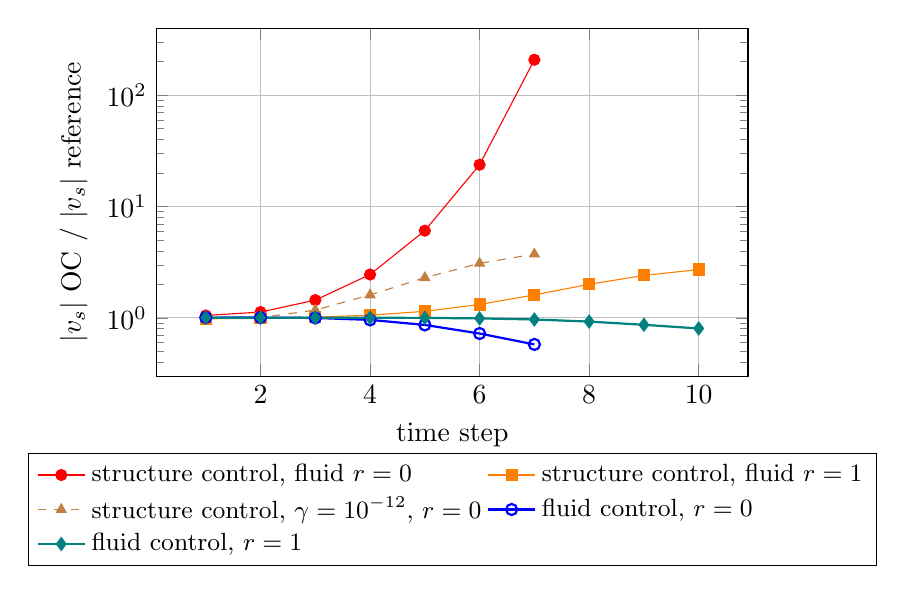
\begin{tikzpicture}
\begin{semilogyaxis}[width=0.75\textwidth,height=6cm,xlabel={time step},
  ylabel={$|v_s|$ OC / $|v_s|$ reference},legend cell align=left,
  legend style={at={(0.5,-0.22)},anchor=north,legend columns=2,font=\small},
  ymin=0.3,ymax=400,grid=major]
\addplot+[red,mark=*,mark options={fill=red}] coordinates {(1,1.052)(2,1.129)(3,1.445)(4,2.453)(5,6.077)(6,23.77)(7,208.4)};
\addlegendentry{structure control, fluid $r=0$}
\addplot+[orange,mark=square*,mark options={fill=orange}] coordinates {(1,0.982)(2,0.991)(3,1.015)(4,1.057)(5,1.146)(6,1.320)(7,1.609)(8,2.003)(9,2.409)(10,2.717)};
\addlegendentry{structure control, fluid $r=1$}
\addplot+[brown,dashed,mark=triangle*,mark options={fill=brown,solid}] coordinates {(1,0.983)(2,1.006)(3,1.176)(4,1.608)(5,2.298)(6,3.089)(7,3.744)};
\addlegendentry{structure control, $\gamma=10^{-12}$, $r=0$}
\addplot+[blue,thick,mark=o] coordinates {(1,1.006)(2,1.007)(3,0.999)(4,0.960)(5,0.865)(6,0.724)(7,0.578)};
\addlegendentry{fluid control, $r=0$}
\addplot+[teal,thick,mark=diamond*,mark options={fill=teal}] coordinates {(1,1.004)(2,1.004)(3,1.004)(4,1.003)(5,1.000)(6,0.990)(7,0.968)(8,0.927)(9,0.867)(10,0.804)};
\addlegendentry{fluid control, $r=1$}
\end{semilogyaxis}
\end{tikzpicture}
\caption{Velocity-mismatch formulation: norm of the structure velocity relative to the reference
(IQN-ILS, tolerance $10^{-10}$, same mesh).}\label{fig:stability}
\end{figure}

\paragraph{Fluid trace and a common interface space}

With the control in the trace of the DG fluid velocity space (40 against 130 interface degrees of
freedom at $r=0$) the scheme is stable, the control coincides with the fluid traction within
$0.7\%$, and the problem is better conditioned (GN: 2 iterations, 79 tangent solves). As a common,
coarser interface space we also use discontinuous polynomials of degree $k_f-\rho$ on the fluid
faces of $\G$, with a face-wise $L^2$ projection $P_c$ (self-adjoint in $\M$). The effect on the
solution is small (\cref{tab:common}).

\begin{table}[ht]\centering
\caption{Common interface space, fluid refinement 0: tip displacement $d_x(0.01)$ relative to the
reference.}\label{tab:common}
\begin{tabular}{lcc}
\toprule
control space & dimension & ratio\\
\midrule
fluid trace, degree 3 & 40 & 0.778\\
degree 2 & 30 & 0.782\\
degree 1 & 20 & 0.784\\
degree 0 & 10 & 0.867\\
\bottomrule
\end{tabular}
\end{table}

\subsubsection{Diagnosis of the remaining discrepancy}\label{sec:diagnosis}

With fluid control the velocity-mismatch formulation is stable but differs from the reference by
$22\%$ at refinement 0 in the tip displacement. We isolate the cause.

\paragraph{Convergence.} Refining fluid and structure, the ratio approaches one at first order
(\cref{tab:hstudy}); Richardson extrapolation of the OC values gives $-1.43\cdot10^{-7}$, within
$1.5\%$ of the reference.

\begin{table}[ht]\centering
\caption{Tip displacement $d_x$ at $t=0.01$ (log-linear interpolation in time).}\label{tab:hstudy}
\begin{tabular}{cccc}
\toprule
refinement & reference & OC (fluid control) & ratio\\
\midrule
0 & $-1.4635\cdot10^{-7}$ & $-1.1389\cdot10^{-7}$ & 0.778\\
1 & $-1.4745\cdot10^{-7}$ & $-1.3014\cdot10^{-7}$ & 0.883\\
2 & $-1.4540\cdot10^{-7}$ & $-1.3738\cdot10^{-7}$ & 0.945\\
\bottomrule
\end{tabular}
\end{table}

\paragraph{Separation of effects.} The discrepancy is independent of the time step (CFL $0.5$,
$0.25$, $0.125$: ratios $0.778$, $0.781$, $0.782$), of the structure mesh (fluid refinement 0:
$0.778$ and $0.781$ for structure refinement 0 and 1; fluid refinement 1: $0.885$ and $0.883$;
fluid refinement 2: $0.950$ and $0.945$) and of the geometry treatment (explicit geometry and ten
fixed-point iterations on the geometry, converged to $10^{-12}$, give identical results). It
depends only on the fluid mesh. The treatment of the convective term on $\G$ (outflow/backflow
versus moving wall) has no effect, since $(u-w)\cdot n\approx0$ on the interface, and the pressure
term is consistent ($\{p\}=p_\G$).

\paragraph{Force decomposition.} \Cref{tab:faces} compares, face by face, the force computed from
the fluid solution, $\int\rho_f(\nu F(u)-pI)n_f$, with the force imposed through the control,
$-\int g$, at $t\approx0.008$ and refinement 0. The fluid solutions of OC and DN coincide within
$1\%$ (pressure force $0.4766$ against $0.4794$). On the tip both forces agree; on the long sides of
the flag the tangential component of the control is 20 to 90 times the viscous stress computed
from the velocity gradient. The deficit of the transmitted force ($0.354$ against $0.474$ in $x$)
is exactly the observed deviation.

\begin{table}[ht]\centering
\caption{Forces on the fluid at $t=7.96\cdot10^{-3}$, refinement 0, $x$ components.}
\label{tab:faces}
\begin{tabular}{lccc}
\toprule
face & length & from fluid solution & imposed ($-\int g$)\\
\midrule
tip ($x=0.6$) & 0.020 & $0.4765$ & $0.4678$\\
upper side, first face & 0.151 & $-0.00066$ & $-0.0147$\\
lower side, first face & 0.151 & $-0.00064$ & $-0.0155$\\
upper side, second face & 0.200 & $-0.00049$ & $-0.0410$\\
lower side, second face & 0.200 & $-0.00047$ & $-0.0430$\\
\bottomrule
\end{tabular}
\end{table}

\paragraph{Boundary layer.} Following the shear force on the long sides under refinement
(\cref{fig:shear}): the force imposed by the multiplier \emph{decreases}
($-0.114,-0.034,-0.026,-0.020$), the viscous stress of the DN solution \emph{increases}
($-0.0004,-0.0010,-0.0038,-0.0091$), and both approach a common value of about $-0.012$; the tip
ratio reaches $0.98$ at refinement 3.

\begin{figure}[ht]\centering
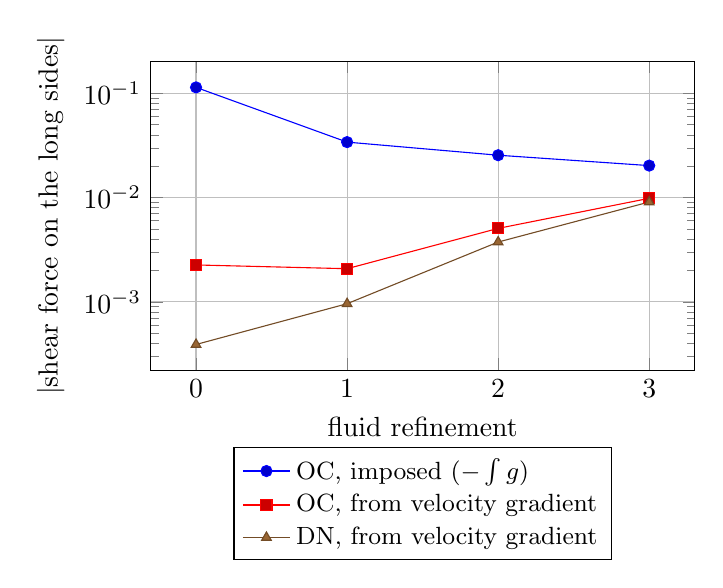
\begin{tikzpicture}
\begin{semilogyaxis}[width=0.7\textwidth,height=5.5cm,xlabel={fluid refinement},
  ylabel={$|$shear force on the long sides$|$},xtick={0,1,2,3},legend cell align=left,
  legend style={at={(0.5,-0.25)},anchor=north,font=\small},grid=major]
\addplot+[mark=*] coordinates {(0,0.1142)(1,0.03409)(2,0.02552)(3,0.02029)};
\addlegendentry{OC, imposed ($-\int g$)}
\addplot+[mark=square*] coordinates {(0,0.00226)(1,0.00208)(2,0.00507)(3,0.00985)};
\addlegendentry{OC, from velocity gradient}
\addplot+[mark=triangle*] coordinates {(0,0.00039)(1,0.00096)(2,0.00375)(3,0.00908)};
\addlegendentry{DN, from velocity gradient}
\end{semilogyaxis}
\end{tikzpicture}
\caption{Shear force on the long sides of the flag at the last time step before $t=0.008$.}
\label{fig:shear}
\end{figure}

\paragraph{Interpretation.} The two schemes impose the no-slip condition differently. In the
velocity-mismatch formulation the multiplier enforces it strongly (the fluid trace equals
$\Pi v_s$), and on an unresolved boundary layer the discrete flux needed to do so overestimates the
wall shear. In the native DN scheme the condition is imposed weakly by SIPG, whose penalty scales
with $\nu$; at Reynolds numbers of order $10^2$ the fluid effectively slips on coarse meshes, and the
shear computed from the velocity gradient is underestimated. This is the dichotomy between strong
and weak imposition of Dirichlet conditions on unresolved boundary layers
\cite{BazilevsHughes2007}. The DN scheme \emph{appears} mesh converged only because the
$x$ force is dominated by the pressure on the tip; both schemes converge to the same limit.

\paragraph{Unsuccessful remedies.} (i) A stabilisation of the constraint row only, in the spirit of
Stenberg \cite{Stenberg1995} and Barbosa--Hughes \cite{BarbosaHughes1991},
$m=\Pi(u_f-v_s)-\beta\Pi(T_f(u_f,p_f)+g)$ with $\beta=\alpha h_F/(k\mu_f)$, is consistent and has
an exact adjoint, but is unstable for every $\alpha\neq0$ (tip ratios $0.51$, $-8.1$, $-160$,
$8.4$ for $\alpha=0.1,1,10,-1$); the full method also modifies the fluid equation. (ii) A Robin
penalty $\nu\beta(u-v_s)$ on the fluid side combined with a coarse common space changes the result
by less than $0.5\%$: $\nu\beta\ll1/\Delta t$, and the face means of the no-slip condition remain
imposed by the multiplier. (iii) For the full fluid trace, any penalty tested on the same trace
vanishes identically at convergence by the orthogonality of $\Pi$.

\subsection{The native-traction formulation}\label{sec:res_native}

\paragraph{Results.} With interface Newton the solution coincides with the reference to all digits
reported (ratio $1.0000$ at refinements 0 and 1), and Newton converges quadratically
($\|m\|$: $1.6$, $6.0\cdot10^{-4}$, $7.9\cdot10^{-7}$, $5.8\cdot10^{-9}$). The tangent-based
variants with finite-difference tangents are expensive; the secant method of \cref{alg:qn}
requires no tangent solves at all and is as fast as IQN-ILS (\cref{tab:native}; between the two
sessions the relative timing varied between $0.57$ and $1.0$ with the load of the machine, see
\cref{tab:native_methods} for a run under identical load). Two safeguards were necessary in the added-mass
regime: a QR filter ($\epsilon=10^{-4}$) and a restart that discards only the pairs of previous
time steps (pure relaxation with $\omega_0=0.3$ diverges, with residual growth factors 2 and 9 at
refinements 0 and 1).

\begin{table}[ht]\centering
\caption{Native-traction formulation, 4 processes; ratio of $d_x(0.01)$ to the reference.}
\label{tab:native}
\resizebox{\textwidth}{!}{%
\begin{tabular}{lccccc}
\toprule
& \multicolumn{2}{c}{refinement 0 (5 steps)} & \multicolumn{2}{c}{refinement 1 (8 steps)} & \\
\cmidrule(lr){2-3}\cmidrule(lr){4-5}
method & time & solves/step & time & solves/step & ratio\\
\midrule
IQN-ILS (native, reference) & 4.40 s & 10.4 & 25.1 s & 11.3 & ---\\
IQN (\cref{alg:qn}) & \textbf{3.95 s} & 8.8 & \textbf{14.2 s} & 10.4 & 1.0000\\
IN, frozen Jacobian, central FD & 38.2 s & 5.0 + 68 fluid & 126 s & 4.9 + 83 fluid & 1.0000\\
IN, frozen Jacobian, forward FD & 20.4 s & 4.8 + 34 fluid & 74.9 s & 4.8 + 41 fluid & 1.0000\\
\bottomrule
\end{tabular}}
\end{table}




\paragraph{All methods on the native solution.} \Cref{tab:native_methods} repeats the comparison of
\cref{sec:results_methods} for the native formulation. All converged methods reproduce the
reference tip displacement to six digits. The native operator $S=I-\M^{-1}G$ is much better
conditioned than in the velocity-mismatch formulation: Gauss--Newton needs about nine CG iterations
per step instead of hundreds, and interface Newton three GMRES iterations. The ranking predicted by
the scalar model is confirmed: the secant method and interface Newton are cheapest, the
normal-equation methods (GN, LM, TR) cost five to six times more solves than interface Newton,
L-BFGS converges but needs about sixty iterations, and steepest descent does not converge within
200 iterations.

\begin{table}[ht]\centering
\caption{Native formulation, refinement 0, average per time step over four steps (tolerance
$\|m\|\le10^{-8}$); one state evaluation = structure Newton solve, ALE update and fluid step;
$S$, $S^*$ = one linearised structure solve and one linear fluid solve each. Times: five steps,
refinement 0 and 1 (structure refinement 0), four simultaneous runs with 4 processes.}
\label{tab:native_methods}
\resizebox{\textwidth}{!}{%
\begin{tabular}{lccccccc}
\toprule
method & iterations & states & $S$ & $S^*$ & $d_x$ error & time $r=0$ & time $r=1$\\
\midrule
IQN-ILS (native) & 10.4 & 10.4 & -- & -- & --- & 4.70 s & 24.8 s\\
interface quasi-Newton & 7.8 & 8.8 & 0 & 0 & $<10^{-6}$ & 4.32 s & 24.4 s\\
interface Newton & 4.0 & 5.0 & 12.2 & 0 & $<10^{-6}$ & 9.57 s & 48.7 s\\
Gauss--Newton & 4.5 & 5.5 & 38 & 44 & $<10^{-6}$ & 47.0 s & 146 s\\
trust region & 4.75 & 5.75 & 40 & 46 & $<10^{-6}$ & & \\
Levenberg--Marquardt & 4.75 & 5.75 & 48 & 49 & $<10^{-6}$ & & \\
L-BFGS & 62 & 78 & 1 & 63 & $<10^{-6}$ & & \\
steepest descent & 200 (limit) & 201 & 200 & 200 & $11\%$ & & \\
\bottomrule
\end{tabular}}
\end{table}

\subsection{Reducing the cost of the secant solver}\label{sec:speedup}

In all configurations above more than $95\%$ of the run time is spent in the linear solves of the
fluid step; the interface algebra, the structure and the ALE update are negligible. We therefore
examine three ways to reduce the cost of \cref{alg:qn} on the native formulation: cheaper state
evaluations (\cref{sec:inexact}), a cheaper fluid solver (\cref{sec:splitting}) and fewer state
evaluations (\cref{sec:initial_jacobian}). All runs in this section use fluid refinement 1,
structure refinement 0, $t\in[0,0.02]$ (11 time steps) and 4 processes; wall times are only
comparable within one group of simultaneous runs, so every table reports runs started together.

\subsubsection{Inexact state evaluations and the noise floor of the state map}\label{sec:inexact}

\paragraph{Warm start.} The fluid step is solved by FGMRES with absolute tolerance $10^{-14}$ and
relative tolerance $10^{-10}$, starting from the extrapolation in time. Within one time step,
consecutive state evaluations differ only slightly, so starting the fluid solve from the previous
evaluation (as the Dirichlet--Neumann iteration of ExaDG does after its first iteration) reduces
the iterations per solve from about $45$ to $28$. Used naively, however, the warm start
\emph{increases} the number of secant iterations from $9$ to $50$ per step. Two mechanisms are
responsible, and both are worth stating since they apply to any secant method acting on a
black-box time step.

\begin{enumerate}
\item \emph{The discrete operator depended on the initial guess.} When ExaDG does not extrapolate,
it computes the penalty parameters of the divergence and continuity penalty terms, which depend on
the local velocity magnitude, from the previous iterate instead of from the extrapolated velocity.
The state map then depends on the history of the iteration, not only on $g$. For a fixed-point
iteration this is harmless (the parameters converge with the iterate), but a secant method
interprets the change of the operator as a change of the Jacobian. We added an opt-in switch
\code{TimeIntBDF::set_penalty_velocity_from_extrapolation} that keeps the extrapolated velocity
for the penalty parameters while still using the previous iterate as initial guess; it is enabled
only by the optimal-control coupling, so the native schemes are unchanged.
\item \emph{Absolute tolerances suppress small responses.} The Newton solver of the structure
stops before the first iteration if the residual of the initial guess is below its absolute
tolerance. With a warm start and a small change of $g$ this happens frequently: the structure does
not respond at all and the secant pair is wrong. The structure (about $2\%$ of the cost) therefore
always starts from the extrapolation; only the fluid is warm-started.
\end{enumerate}

With both corrections the secant method still stagnates at $\|m\|\approx10^{-8}$ in some time
steps, for the reason given in \cref{rem:noise}.



For the coupled fluid solver with tolerances $10^{-14}/10^{-10}$ the noise floor is
$\varepsilon\approx10^{-8}$ in $\|m\|$ (with $\|m_0\|$ between $1$ and $17$), that is round-off level
of the saddle-point solve. The cold-start runs with tolerance $10^{-8}$ are not more accurate than
this: they only satisfy a consistent perturbation of the interface equation. With the tolerance
$10^{-7}$ the solutions of all variants agree with the $10^{-8}$ cold-start solution to
$7\cdot10^{-8}$ relative in the tip displacement (\cref{tab:inexact}).

\paragraph{Adaptive inner tolerance.} In the spirit of inexact Newton methods
\cite{DemboEisenstatSteihaug1982} the relative tolerance of the fluid solve is relaxed while the
interface residual is large,
\begin{equation}\label{eq:adaptive_tol}
  \eta_k=\max\Big(\eta,\ \min\big(10^{-2},\ \eta\,\min(10^8,\max(1,\
  \sigma\,\|m_k\|/\mathrm{tol}))\big)\Big),\qquad \sigma=10^{-2},
\end{equation}
where $\eta$ is the nominal relative tolerance and $\mathrm{tol}$ the interface tolerance; the
absolute tolerance is not scaled (scaling it truncated the fluid solves at small displacement
amplitudes and produced wrong solutions). On its own, \eqref{eq:adaptive_tol} does not pay off: the
evaluations become cheaper, but the changing solver error makes the state map inconsistent in the
sense of \cref{rem:noise} and the secant method needs more iterations. Together with the warm start
the inexact early evaluations cost only a few FGMRES iterations each.

\begin{table}[ht]\centering
\caption{Inexact state evaluations, native formulation, coupled fluid solver, interface tolerance
$10^{-7}$; four simultaneous runs. ``FGMRES'' is the average number of iterations per fluid solve;
the last column is the maximum relative deviation of the tip displacement from the cold-start
solution with tolerance $10^{-8}$.}\label{tab:inexact}
\begin{tabular}{lcccc}
\toprule
variant & wall time & states/step & FGMRES & deviation\\
\midrule
cold start, fixed tolerance & 27.4 s & 9.2 & 44.9 & $1.7\cdot10^{-8}$\\
warm start (fluid) & 18.2 s & 10.9 & 28.1 & $7.1\cdot10^{-8}$\\
adaptive tolerance & 28.1 s & 12.6 & 31.2 & $5.2\cdot10^{-9}$\\
warm start + adaptive tolerance & \textbf{15.9 s} & 10.2 & 22.1 & $2.6\cdot10^{-8}$\\
\bottomrule
\end{tabular}
\end{table}

\paragraph{Comparison with IQN-ILS.} The Dirichlet--Neumann IQN-ILS reference stops when the
displacement residual is below $\mathrm{AbsTol}\sqrt{n}$ or $\mathrm{RelTol}\,\|v_s\|\Delta t$. With
$\mathrm{AbsTol}=10^{-14}$ it needs $17.2$ iterations per step on this interval; relaxing the
absolute tolerance saves iterations but costs accuracy ($12.5$ iterations and a deviation of
$4.9\cdot10^{-3}$ for $10^{-12}$, $10.2$ iterations and $2.4\cdot10^{-2}$ for $10^{-11}$), because
the displacements during the start-up are of order $10^{-10}$ to $10^{-6}$. At equal accuracy the
secant method on the native formulation with warm start and adaptive tolerance is $2.4$ times faster
(\cref{tab:speedup}).

\subsubsection{A cheaper fluid solver}\label{sec:splitting}

The derivatives of \cref{sec:native_adjoint} require the coupled fluid solver, whose system matrix
is the symmetric saddle-point matrix. \Cref{alg:qn} needs no derivatives, so on the native
formulation it can use any time integrator of ExaDG, in particular the dual-splitting scheme with
its standard solver tolerances ($10^{-8}$ absolute, $10^{-6}$ relative). In this configuration a
fluid step costs about three pressure-Poisson and five viscous CG iterations. The splitting changes
the fluid discretisation: the tip displacement at $t=0.02$ differs from the coupled solution by
$1.4\cdot10^{-3}$ relative.

The loose single-field tolerances raise the noise floor of \cref{rem:noise} accordingly. The warm
start must therefore not be used with the splitting scheme (the secant method then stagnates at
about $10^{-6}$), while the cold-start secant method is insensitive to it. IQN-ILS warm-starts both
fields after its first iteration, so its result depends on the inexactness of the fluid solves
(\cref{sec:fluid_accuracy}). In addition, its stopping criterion is effectively absolute during the
start-up, where the displacements are of order $10^{-11}$ to $10^{-6}$ (\cref{tab:splitting}): with
the tolerances of the standard input of the application ($\mathrm{AbsTol}=10^{-8}$,
$\mathrm{RelTol}=10^{-3}$) the first time steps are accepted after a single Dirichlet--Neumann
pass and the tip displacement is wrong by a factor $46$ (the error decays and is below $1\%$ from
$t\approx0.03$ on); with $10^{-11}/10^{-6}$ it needs $13.4$ iterations for a deviation of
$4\cdot10^{-3}$; with $\mathrm{AbsTol}=10^{-14}$ the original implementation diverged in the third
time step (see \cref{sec:iqn_fix} for the modifications). The secant method reaches a deviation of
$2.4\cdot10^{-6}$ with $7.9$ state evaluations per step.

\begin{table}[ht]\centering
\caption{Dual-splitting fluid solver, $t\in[0,0.02]$: iterations per time step and maximum and
final relative deviation of the tip displacement from the secant solution with tolerance $10^{-7}$
(cold start). IQN-ILS before the modifications of \cref{sec:iqn_fix}.}
\label{tab:splitting}
\begin{tabular}{lccc}
\toprule
method, tolerance & iterations & max.\ deviation & final deviation\\
\midrule
IQN-ILS, $10^{-8}/10^{-3}$ & 21.1 & $46$ & $46$\\
IQN-ILS, $10^{-11}/10^{-6}$ & 13.4 & $9.7\cdot10^{-2}$ & $4.3\cdot10^{-3}$\\
IQN-ILS, $10^{-14}/10^{-10}$ & \multicolumn{3}{c}{diverges in time step 3}\\
secant, $10^{-4}$ & 7.9 & $1.2\cdot10^{-4}$ & $2.4\cdot10^{-6}$\\
secant, $10^{-5}$ & 8.6 & $7.5\cdot10^{-6}$ & $1.8\cdot10^{-9}$\\
secant, $10^{-7}$ & 10.1 & -- & --\\
\bottomrule
\end{tabular}
\end{table}

\begin{table}[ht]\centering
\caption{Summary, four simultaneous runs: total wall time, wall time of the time loop and
iterations (state evaluations) per time step. The dual-splitting run solves a different fluid
discretisation (deviation $1.4\cdot10^{-3}$).}\label{tab:speedup}
\begin{tabular}{lcccc}
\toprule
configuration & total & time loop & iterations & speed-up\\
\midrule
IQN-ILS, coupled fluid, $10^{-14}/10^{-10}$ & 36.2 s & 34.8 s & 17.2 & 1.0\\
secant, coupled fluid, cold start & 23.7 s & 22.5 s & 9.2 & 1.5\\
secant, coupled fluid, warm start + adaptive & 16.0 s & 14.8 s & 10.2 & 2.4\\
secant, dual splitting, $10^{-5}$ & 2.1 s & 0.8 s & 8.6 & $\approx40$\\
\bottomrule
\end{tabular}
\end{table}

\subsubsection{Initial Jacobians}\label{sec:initial_jacobian}

Neither pays off during the start-up phase. With \eqref{eq:imvj} the secant method needs
$10.1$ evaluations per step without reuse of old pairs and $16.4$ with reuse of eight steps, against
$9.0$ and $10.2$ for $H_0=\omega I$: the Jacobian changes too quickly between time steps. (Reusing
the pairs of previous steps does not help either here.) The frozen Jacobian reduces the evaluations
to $6.9$ per step, but its assembly costs $2\times130$ tangent solves per refresh, i.e.\ about
$24$ per step, and the run takes $78$~s instead of $10$~s. Both options are meant for the periodic
regime, where the Jacobian changes slowly and the refresh interval can be long.

\subsection{Long simulations of FSI2}\label{sec:longruns}

We now run the FSI2 configuration over the end time of the ExaDG application, $T=4L/U=10$~s,
and beyond, with the dual-splitting fluid solver (the default of the application). Two
resolutions are used: fluid $Q_3$ with one refinement and structure $Q_2$ without refinement (the
resolution of the previous sections), and fluid $Q_6$, structure $Q_4$, both without refinement
(the resolution of the Aitken input of the application). Each run uses 4 processes; the time step
is adaptive (CFL $0.5$), about $4150$ and $5900$ steps for $10$~s, respectively. The tip
displacement is recorded at point $A=(0.6,0.2)$ in every time step.

\subsubsection{Robustness of IQN-ILS}\label{sec:iqn_fix}

With the coarser resolution and the tolerances of the standard input ($\mathrm{AbsTol}=10^{-8}$,
$\mathrm{RelTol}=10^{-3}$, eight reused time steps, $\omega_0=0.3$), the IQN-ILS implementation of
ExaDG diverged at $t\approx0.055$ (the damped Newton solver of the structure failed). Aitken
relaxation with the same tolerances, IQN-ILS at the finer resolution, and IQN-ILS with zero or one
reused time step, with $\omega_0=0.5$ or with $\mathrm{AbsTol}=10^{-12}$ all ran through. The
mechanism is the one of \cref{sec:splitting}: during the start-up the absolute criterion accepts
the first Dirichlet--Neumann pass, and the secant pairs of these non-converged steps are reused for
eight steps. The implementation appended the reused columns oldest first, and the QR filter, which
drops a column that is nearly dependent on the preceding ones, therefore kept the oldest
information. We changed two points:
\begin{enumerate}
\item the columns are assembled newest first (current step, newest iteration first, then the
reused steps, newest first), so that outdated columns are the ones filtered out; this alone removes
the divergence;
\item if the residual grows by more than a factor (\code{FSI/IQNRestartFactor}, default $2$)
within a partitioned iteration, the pairs of the previous time steps are discarded.
\end{enumerate}
With these changes the standard-tolerance run completes the $10$~s with $2.52$ iterations per step,
and the run with $10^{-11}/10^{-6}$ needs $3.32$ instead of $3.78$ iterations per step with an
unchanged solution (deviation $\le2\cdot10^{-3}$).

\subsubsection{Accuracy of the fluid solves}\label{sec:fluid_accuracy}

Over $10$~s, the converged secant solution and the converged Dirichlet--Neumann solution first
seemed to differ by up to $30\%$ in the tip displacement. The difference is not a property of the
formulations. It is already present after the first time step, where the vertical displacement is
of order $10^{-13}$ and consists of numerical noise that breaks the symmetry of the flow; the FSI2
instability grows from this seed, so that its phase depends on perturbations at round-off level.
The noise comes from the linear solvers of the dual-splitting scheme, whose absolute tolerance
$10^{-8}$ dominates during the start-up. Tightening the fluid tolerances to $10^{-12}/10^{-9}$
(parameters \code{FluidSolverAbsTol}, \code{FluidSolverRelTol} of the application) makes the two
schemes coincide (\cref{tab:fluid_tol_startup}).

\begin{table}[ht]\centering
\caption{Relative difference of the tip displacement between the converged secant solution
($\|m\|\le10^{-9}$) and the converged Dirichlet--Neumann solution ($\mathrm{RelTol}=10^{-10}$),
fluid $Q_3$, refinement 1. Each scheme is converged with respect to its own tolerance (tolerances
$10^{-9}$ and $10^{-11}$, resp.\ $10^{-8}$ and $10^{-10}$, give the same digits).}
\label{tab:fluid_tol_startup}
\begin{tabular}{ccccc}
\toprule
& \multicolumn{2}{c}{fluid tolerances $10^{-8}/10^{-6}$} & \multicolumn{2}{c}{fluid tolerances $10^{-12}/10^{-9}$}\\
step & $d_x$ & $d_y$ & $d_x$ & $d_y$\\
\midrule
1 & $1.4\cdot10^{-3}$ & $9.5\cdot10^{-2}$ & $6.1\cdot10^{-7}$ & $6.5\cdot10^{-5}$\\
2 & $5.9\cdot10^{-2}$ & $1.5\cdot10^{-1}$ & $1.5\cdot10^{-5}$ & $2.9\cdot10^{-4}$\\
9 & $4.2\cdot10^{-3}$ & $9.1\cdot10^{-1}$ & $5.8\cdot10^{-7}$ & $1.3\cdot10^{-4}$\\
16 & $6.3\cdot10^{-4}$ & $6.6\cdot10^{-2}$ & $1.6\cdot10^{-7}$ & $1.9\cdot10^{-4}$\\
\bottomrule
\end{tabular}
\end{table}

Over the whole simulation the two schemes react very differently to the inexact fluid solves
(\cref{tab:fluid_tol_long}). The secant method starts every fluid solve from the extrapolation in
time, so the solver error is consistent in the sense of \cref{rem:noise}; with the default fluid
tolerances it stays within $3\cdot10^{-4}$ of the accurate solution. The Dirichlet--Neumann
iteration restarts the fluid solvers from the previous iterate, whose residual is often already
below the absolute tolerance; the fluid then hardly responds to small changes of the interface
velocity, and the fixed point depends on the iteration path. Accordingly, its deviation grows with
the number of warm-started iterations: $3\%$ for IQN-ILS with the standard tolerances ($2.7$
iterations per step), $17\%$ for Aitken ($5.8$) and $30\%$ for IQN-ILS with tight tolerances
($3.5$). A tight Dirichlet--Neumann tolerance is therefore
only meaningful together with accurate fluid solves.

\begin{table}[ht]\centering
\caption{Fluid $Q_6$, structure $Q_4$: maximum deviation of $d_y(A)$ from the Dirichlet--Neumann
solution with accurate fluid solves ($10^{-12}/10^{-9}$, IQN-ILS $10^{-11}/10^{-6}$), relative to
the maximum of $|d_y|$ in each time window. The reference run stopped at $t=8.88$ because the
pressure-Poisson solver could not reach the absolute tolerance $10^{-12}$ at large amplitudes.}
\label{tab:fluid_tol_long}
\resizebox{\textwidth}{!}{%
\begin{tabular}{llccccc}
\toprule
method & fluid tolerances & $[0,2)$ & $[2,4)$ & $[4,6)$ & $[6,8)$ & $[8,8.88]$\\
\midrule
secant, $\|m\|\le10^{-5}+10^{-6}\|g\|$ & $10^{-12}/10^{-9}$ & $1.3\cdot10^{-5}$ & $3.6\cdot10^{-5}$ & $1.0\cdot10^{-4}$ & $1.6\cdot10^{-4}$ & $1.4\cdot10^{-4}$\\
secant, $\|m\|\le10^{-5}$ & default & $8.6\cdot10^{-5}$ & $1.0\cdot10^{-4}$ & $1.7\cdot10^{-4}$ & $2.4\cdot10^{-4}$ & $2.3\cdot10^{-4}$\\
secant, $\|m\|\le10^{-5}\max(1,\|g\|)$, stagnation stop & default & $9.3\cdot10^{-5}$ & $1.2\cdot10^{-4}$ & $2.3\cdot10^{-4}$ & $3.1\cdot10^{-4}$ & $3.1\cdot10^{-4}$\\
IQN-ILS, $10^{-8}/10^{-3}$ & default & $2.8\cdot10^{-3}$ & $7.2\cdot10^{-3}$ & $2.9\cdot10^{-2}$ & $3.4\cdot10^{-2}$ & $2.8\cdot10^{-2}$\\
Aitken, $10^{-8}/10^{-3}$ & default & $5.7\cdot10^{-3}$ & $4.5\cdot10^{-2}$ & $1.4\cdot10^{-1}$ & $1.6\cdot10^{-1}$ & $1.7\cdot10^{-1}$\\
IQN-ILS, $10^{-11}/10^{-6}$ & default & $1.6\cdot10^{-2}$ & $6.7\cdot10^{-2}$ & $1.9\cdot10^{-1}$ & $3.0\cdot10^{-1}$ & $2.7\cdot10^{-1}$\\
\bottomrule
\end{tabular}}
\end{table}

\subsubsection{Stopping criteria of the secant method}\label{sec:stopping}

At the finer resolution the secant method with the absolute tolerance $\|m\|\le10^{-5}$ needed
$22.8$ state evaluations per step on average, five times as long as IQN-ILS. A run with iteration
output shows why: between $t=2$ and $t=7$ it needs $3.4$ to $4.7$ evaluations per step, but during
the start-up and when the amplitude grows it stagnates at $\|m\|\approx2\cdot10^{-5}$ to
$3\cdot10^{-4}$, just above the tolerance, and $96$ steps reach the limit of $200$ iterations.
With $Q_6$ elements the stress amplifies the error of the fluid solves, and the noise floor of the
state map (\cref{rem:noise}) exceeds the absolute tolerance. Two options remedy this:
\begin{itemize}
\item \code{MismatchToleranceRelative}: stop if $\|m\|_\M\le\max(\mathrm{tol},\
\mathrm{rtol}\,\|g\|_\M)$, i.e.\ relative to the size of the traction (the analogue of the relative
criterion of the Dirichlet--Neumann iteration; the interface forces are between $3$ and
$30$~N/m here);
\item \code{StagnationIterations}: stop if the smallest residual has not decreased by $10\%$
within $N$ iterations, and return the best iterate.
\end{itemize}
With $\mathrm{rtol}=10^{-5}$ and $N=10$ the secant method needs $2.20$ evaluations per step and
$376$~s instead of $1653$~s, with the accuracy of \cref{tab:fluid_tol_long}; with accurate fluid
solves and $\mathrm{rtol}=10^{-6}$ it needs $2.55$ evaluations and $424$~s. For comparison, in a
different group of simultaneous runs IQN-ILS needed $2.69$ iterations and $316$~s (standard
tolerances), $3.45$ and $338$~s (tight tolerances), and Aitken $5.77$ and $469$~s. The secant method
needs fewer state evaluations than IQN-ILS, but each one starts from the extrapolation and costs
more fluid iterations; at equal accuracy (accurate fluid solves for the Dirichlet--Neumann
iteration) the costs are comparable.

\subsubsection{Periodic regime and comparison with the benchmark}\label{sec:benchmark}

To reach the periodic regime we extend the simulation to $t=25$~s (fluid $Q_6$, structure $Q_4$)
and compare four couplings: the secant method on the native formulation with the stopping
criteria of \cref{sec:stopping} and the default fluid tolerances, IQN-ILS with the standard
tolerances, Aitken relaxation with the input of the application, and IQN-ILS with tight
tolerances and accurate fluid solves ($10^{-10}/10^{-9}$). For each period of $d_y(A)$, delimited
by two upward zero crossings, we record the mean, the amplitude (half the peak-to-peak value) and
the frequency. The reference values are those of Turek and Hron \cite{TurekHron2006} for FSI2:
$d_x(A)=(-14.58\pm12.44)\cdot10^{-3}$ at $3.8$~Hz and $d_y(A)=(1.23\pm80.6)\cdot10^{-3}$ at
$2.0$~Hz (quoted from memory, see the note in the references).

\pgfplotsset{
  fsiqn/.style={blue!70!black, thick},
  fsiiqn/.style={red!75!black, thick, densely dashed},
  fsiaitken/.style={green!50!black, thick, densely dotted},
  fsiacc/.style={orange!90!black, thick, dashdotted},
  fsiref/.style={black, thin, dashed},
}

\begin{figure}[ht]\centering
\begin{tikzpicture}
\begin{axis}[width=0.98\textwidth, height=5.2cm, xlabel={$t$ [s]}, ylabel={$d_y(A)$ [m]},
  xmin=0, xmax=25, ymin=-0.1, ymax=0.1, grid=major, legend pos=south west,
  legend style={font=\scriptsize}, every axis plot/.append style={line width=0.4pt}]
\addplot[fsiqn] table[x=t, y=uy] {data/u25_qn_signal.dat};
\addlegendentry{secant (native traction)}
\addplot[fsiref, domain=0:25] {0.00123+0.0806};
\addlegendentry{Turek--Hron, mean $\pm$ amplitude}
\addplot[fsiref, domain=0:25, forget plot] {0.00123-0.0806};
\end{axis}
\end{tikzpicture}

\begin{tikzpicture}
\begin{axis}[width=0.98\textwidth, height=5.2cm, xlabel={$t$ [s]}, ylabel={$d_y(A)$ [m]},
  xmin=24, xmax=25, ymin=-0.1, ymax=0.1, grid=major,
  legend columns=3, legend style={font=\scriptsize, at={(0.5,1.03)}, anchor=south},
  restrict x to domain=24:25]
\addplot[fsiqn] table[x=t, y=uy] {data/u25_qn_signal.dat};
\addlegendentry{secant}
\addplot[fsiiqn] table[x=t, y=uy] {data/u25_iqn_signal.dat};
\addlegendentry{IQN-ILS}
\addplot[fsiaitken] table[x=t, y=uy] {data/u25_aitken_signal.dat};
\addlegendentry{Aitken}
\addplot[fsiacc] table[x=t, y=uy] {data/u25_iqn_acc_signal.dat};
\addlegendentry{IQN-ILS, accurate fluid}
\addplot[fsiref, domain=24:25] {0.00123+0.0806};
\addlegendentry{Turek--Hron}
\addplot[fsiref, domain=24:25, forget plot] {0.00123-0.0806};
\end{axis}
\end{tikzpicture}
\caption{Vertical tip displacement $d_y(A)$: whole simulation (secant method, top) and the last
second of all four couplings (bottom), with the band mean $\pm$ amplitude of the reference
\cite{TurekHron2006}.}\label{fig:signal}
\end{figure}

\begin{figure}[ht]\centering
\begin{tikzpicture}
\begin{semilogyaxis}[width=0.44\textwidth, height=5.5cm, xlabel={$t$ [s]},
  ylabel={amplitude of $d_y(A)$ [m]}, xmin=0, xmax=25, ymin=1e-3, ymax=0.2, grid=major,
  legend style={font=\scriptsize}, legend pos=south east]
\addplot[fsiqn] table[x=t, y=uyamp] {data/u25_qn_periods.dat};
\addlegendentry{secant}
\addplot[fsiiqn] table[x=t, y=uyamp] {data/u25_iqn_periods.dat};
\addlegendentry{IQN-ILS}
\addplot[fsiaitken] table[x=t, y=uyamp] {data/u25_aitken_periods.dat};
\addlegendentry{Aitken}
\addplot[fsiacc] table[x=t, y=uyamp] {data/u25_iqn_acc_periods.dat};
\addlegendentry{IQN-ILS, acc.}
\addplot[fsiref, domain=0:25] {0.0806};
\addlegendentry{Turek--Hron}
\end{semilogyaxis}
\end{tikzpicture}\hfill
\begin{tikzpicture}
\begin{axis}[width=0.44\textwidth, height=5.5cm, xlabel={$t$ [s]},
  ylabel={frequency of $d_y(A)$ [Hz]}, xmin=0, xmax=25, ymin=1.6, ymax=2.2, grid=major]
\addplot[fsiqn] table[x=t, y=fuy] {data/u25_qn_periods.dat};
\addplot[fsiiqn] table[x=t, y=fuy] {data/u25_iqn_periods.dat};
\addplot[fsiaitken] table[x=t, y=fuy] {data/u25_aitken_periods.dat};
\addplot[fsiacc] table[x=t, y=fuy] {data/u25_iqn_acc_periods.dat};
\addplot[fsiref, domain=0:25] {2.0};
\end{axis}
\end{tikzpicture}
\caption{Amplitude (left, logarithmic scale) and frequency (right) of $d_y(A)$ per oscillation
period, compared with the periodic values of the reference \cite{TurekHron2006}.}
\label{fig:amplitude_frequency}
\end{figure}

All four runs reach the periodic regime: the amplitude of $d_y(A)$ grows exponentially until
$t\approx10$~s and stays within $1\%$ of its final value from $t\approx11$~s on
(\cref{fig:amplitude_frequency}); the end time $T=10$~s of the application stops just before the
saturation. In the periodic regime the four couplings agree to three or four digits
(\cref{tab:benchmark}), although they differed by up to $30\%$ during the growth phase
(\cref{sec:fluid_accuracy}): the limit cycle is an attractor and forgets the perturbations that
seeded the instability. Compared with the reference, the amplitudes are within $2$ to $5\%$ and the
mean values within $3\%$; the frequency is $1.87$~Hz instead of $2.0$~Hz ($6.7\%$ lower; the
frequency of $d_x$ is exactly twice that of $d_y$ here, whereas the reference values $3.8$ and
$2.0$~Hz are rounded). Since all couplings agree, these deviations are due to the spatial and
temporal discretisation (coarse grid without refinement, CFL $0.5$), not to the coupling; a
resolution study is left for future work.

\begin{table}[ht]\centering
\caption{Periodic regime of FSI2, fluid $Q_6$, structure $Q_4$: mean $\pm$ amplitude
$[\text{frequency}]$ of the tip displacement over the last nine periods ($t\in[20,25]$), compared
with \cite{TurekHron2006}, and cost of the runs over $t\in[0,25]$ (four simultaneous runs with 4
processes each, about $18200$ time steps).}\label{tab:benchmark}
\resizebox{\textwidth}{!}{%
\begin{tabular}{lccccc}
\toprule
& $d_x(A)\ [10^{-3}]$ & $d_y(A)\ [10^{-3}]$ & iterations & wall time\\
\midrule
Turek--Hron \cite{TurekHron2006} & $-14.58\pm12.44\ [3.8]$ & $1.23\pm80.6\ [2.0]$ & & \\
secant, native traction & $-14.17\pm11.80\ [3.73]$ & $1.32\pm79.03\ [1.87]$ & 3.56 & 1591 s\\
IQN-ILS, $10^{-8}/10^{-3}$ & $-14.17\pm11.80\ [3.73]$ & $1.32\pm79.03\ [1.87]$ & 2.84 & 1248 s\\
IQN-ILS, $10^{-11}/10^{-6}$, accurate fluid & $-14.17\pm11.80\ [3.73]$ & $1.32\pm79.03\ [1.87]$ & 3.65 & 1433 s\\
Aitken, $10^{-8}/10^{-3}$ & $-14.14\pm11.79\ [3.73]$ & $1.31\pm79.03\ [1.87]$ & 7.04 & 1920 s\\
\bottomrule
\end{tabular}}
\end{table}

In the large-amplitude regime the secant method needs $3.56$ state evaluations per step (against
$2.2$ over the first $10$~s). It is $27\%$ slower than IQN-ILS with the standard tolerances, $11\%$
slower than IQN-ILS with accurate fluid solves and $17\%$ faster than Aitken relaxation. In the
periodic regime the choice of the coupling therefore affects the cost but not the solution; during
the growth phase, only the secant method and the Dirichlet--Neumann iteration with accurate fluid
solves give the same trajectory.

\subsubsection{Resolution study}\label{sec:resolution}

To identify the source of the remaining deviations from the reference, we vary one discretisation
parameter at a time with respect to the configuration of \cref{sec:benchmark} (fluid $Q_6$ on the
coarse grid with $34$ cells, structure $Q_4$ with $16$ cells, CFL $0.5$), using the secant method
with the stopping criteria of \cref{sec:stopping} up to $t=15$~s and evaluating the periodic
regime on $t\in[12.5,15]$ (the values on $[20,25]$ of the base run agree to $2\cdot10^{-5}$).
\Cref{tab:resolution,fig:resolution} show that the structure is resolved (refining it changes the
results by less than $0.1\%$) and that the frequency is controlled by the spatial resolution of
the fluid: one refinement of the fluid grid raises it from $1.865$ to $1.925$~Hz, the degree $8$
instead of $6$ to $1.906$~Hz, while halving the time step leaves it unchanged. On these grids the amplitude of $d_y$
decreases by about $2\%$ under both fluid and temporal refinement; finer fluid grids, which first
required the remedies of \cref{sec:instabilities}, bring it back to the reference
(\cref{sec:final_comparison}).

\begin{table}[ht]\centering
\caption{Resolution study, periodic regime $t\in[12.5,15]$: mean $\pm$ amplitude
[frequency] of the tip displacement. $N_u$ is the number of velocity degrees of freedom of the
fluid; $\Delta t$ relative to the base run.}\label{tab:resolution}
\resizebox{\textwidth}{!}{%
\begin{tabular}{lcccc}
\toprule
configuration & $N_u$ & $\Delta t/\Delta t_{\mathrm{base}}$ & $d_x(A)\ [10^{-3}]$ & $d_y(A)\ [10^{-3}]$\\
\midrule
Turek--Hron \cite{TurekHron2006} & & & $-14.58\pm12.44\ [3.8]$ & $1.23\pm80.6\ [2.0]$\\
base: fluid $Q_6$, structure $Q_4$, CFL $0.5$ & 3332 & 1 & $-14.17\pm11.82\ [3.73]$ & $1.33\pm79.04\ [1.865]$\\
CFL $0.25$ & 3332 & $0.5$ & $-13.71\pm11.51\ [3.72]$ & $1.32\pm77.60\ [1.863]$\\
structure refined once & 3332 & 1 & $-14.18\pm11.82\ [3.73]$ & $1.33\pm79.10\ [1.865]$\\
fluid $Q_8$ & 5508 & $\approx0.65$ & $-13.11\pm11.16\ [3.82]$ & $0.91\pm76.89\ [1.906]$\\
fluid refined once & 13328 & $0.5$ & $-13.52\pm11.59\ [3.85]$ & $0.98\pm77.52\ [1.925]$\\
\bottomrule
\end{tabular}}
\end{table}

\begin{figure}[ht]\centering
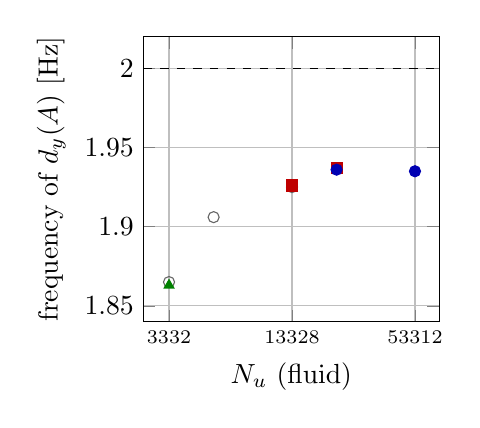
\begin{tikzpicture}
\begin{semilogxaxis}[width=0.44\textwidth, height=5.2cm, xlabel={$N_u$ (fluid)},
  ylabel={frequency of $d_y(A)$ [Hz]}, xmin=2500, xmax=70000, ymin=1.84, ymax=2.02, grid=major,
  xtick={3332,13328,53312}, xticklabels={3332,13328,53312}, xticklabel style={font=\scriptsize}]
\addplot[only marks, mark=o, black!60] coordinates {(3332,1.865) (5508,1.906) (13328,1.925)};
\addplot[only marks, mark=triangle*, green!50!black] coordinates {(3332,1.863)};
\addplot[only marks, mark=square*, red!75!black] coordinates {(13328,1.926) (22032,1.937)};
\addplot[only marks, mark=*, blue!70!black] coordinates {(22032,1.936) (53312,1.935)};
\addplot[black, dashed, domain=2500:70000] {2.0};
\end{semilogxaxis}
\end{tikzpicture}\hfill
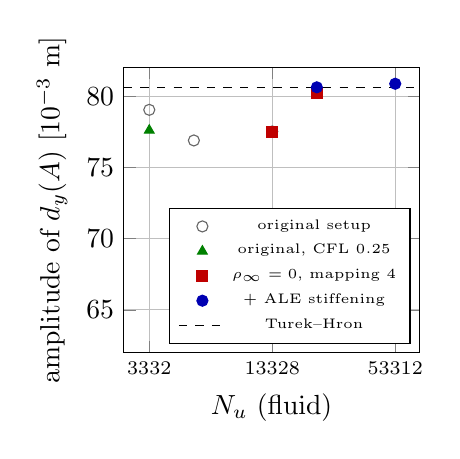
\begin{tikzpicture}
\begin{semilogxaxis}[width=0.44\textwidth, height=5.2cm, xlabel={$N_u$ (fluid)},
  ylabel={amplitude of $d_y(A)$ [$10^{-3}$ m]}, xmin=2500, xmax=70000, ymin=62, ymax=82,
  xtick={3332,13328,53312}, xticklabels={3332,13328,53312}, xticklabel style={font=\scriptsize},
  grid=major, legend style={font=\tiny}, legend pos=south east]
\addplot[only marks, mark=o, black!60] coordinates {(3332,79.04) (5508,76.89) (13328,77.52)};
\addlegendentry{original setup}
\addplot[only marks, mark=triangle*, green!50!black] coordinates {(3332,77.60)};
\addlegendentry{original, CFL $0.25$}
\addplot[only marks, mark=square*, red!75!black] coordinates {(13328,77.46) (22032,80.23)};
\addlegendentry{$\rho_\infty=0$, mapping 4}
\addplot[only marks, mark=*, blue!70!black] coordinates {(22032,80.62) (53312,80.87)};
\addlegendentry{+ ALE stiffening}
\addplot[black, dashed, domain=2500:70000] {80.6};
\addlegendentry{Turek--Hron}
\end{semilogxaxis}
\end{tikzpicture}
\caption{Resolution study: frequency (left) and amplitude (right) of $d_y(A)$ in the periodic
regime against the number of velocity degrees of freedom of the fluid. Original setup: Bossak
$\rho_\infty=0.8$, mapping of the degree of the fluid velocity, band-stiffened mesh motion
($Q_6$ and $Q_8$ without refinement, $Q_6$ refined once); the remedies of
\cref{sec:instabilities} allow the finer grids.}\label{fig:resolution}
\end{figure}

\subsubsection{Two instabilities at fine resolution}\label{sec:instabilities}

The combined refinements (fluid refined twice, fluid $Q_8$ refined once, fluid refined once with
CFL $0.25$) initially diverged. Two distinct phenomena are involved; both are independent of the
coupling algorithm and of the optimal-control formulation.

\paragraph{A. Small time steps.} All runs with $\Delta t\lesssim0.3\,\Delta t_{\mathrm{base}}$
develop an oscillation of the interface traction that grows over several seconds while the
displacement stays smooth (the initial residual of the step, i.e.\ the error of the extrapolated
traction, grows from $1$ at $t\approx2.5$~s to $10^4$ at $t\approx5.6$~s), until the structure
solver fails. With fluid refined once and CFL $0.25$, IQN-ILS fails first ($3.9$~s against $5.4$~s
for the secant method), and tightening the coupling tolerances by two orders of magnitude only
delays the onset. The instability can be reproduced cheaply on the coarsest grid (fluid $Q_3$,
structure $Q_2$, no refinement): with CFL $0.12$ ($\Delta t\approx1.2\cdot10^{-3}$) the run is
stable over $10$~s, with CFL $0.03$ ($\Delta t\approx3\cdot10^{-4}$) it diverges at $t\approx2.2$~s.
The growing component is not a two-step (Nyquist) mode: its period is $8$ to $10$ time steps, i.e.\
about $300$~Hz (about $420$~Hz with a finer structure), and it grows by $1$ to $2\%$ per step. It
is therefore a mode resolved by the time step, with $\omega\Delta t\approx0.6$, far above the
frequency of the flag oscillation ($\approx2$~Hz).

\Cref{tab:instability} summarises the candidate causes tested on the reproducer. Neither the fluid
splitting nor its interface terms are responsible: the coupled fluid solver diverges as well;
replacing the BDF time derivative of the interface velocity in the pressure Neumann condition by
the transferred acceleration of the structure, switching off the penalty terms or their boundary
data, and imposing an interface velocity consistent with the ALE grid velocity do not change the
onset. A richer structure discretisation, which has higher eigenfrequencies, diverges earlier. The
decisive parameter is the numerical dissipation of the structure integrator at
$\omega\Delta t\approx0.6$: the second-order generalized-$\alpha$ schemes with $\rho_\infty\ge0.5$,
whose dissipation there is only of order $(\omega\Delta t)^3$, and the energy-conserving
trapezoidal rule diverge; the first-order Newmark scheme that ExaDG obtains for $\rho_\infty=0.8$
($\gamma=0.61$) and the second-order Bossak and generalized-$\alpha$ schemes with $\rho_\infty=0$
are stable. The Bossak scheme with $\rho_\infty=0$ is the remedy of choice: it remains second
order, its dissipation at the frequency of the flag ($\omega\Delta t\approx0.004$) is negligible,
and the periodic regime of the base run is unchanged ($d_y=1.33\pm79.13$ against $1.33\pm79.04$,
same frequency), whereas the first-order Newmark scheme reduces the amplitude by $0.5\%$. Some
part of the coupled time discretisation still feeds energy into this mode; we have not identified
it, and the structural dissipation only suppresses its effect. For the generalized-$\alpha$ and HHT
schemes part of the instability was caused by the end-of-step load applied at the mid point; with
the consistent mid-point load their onsets move to $1.45$ and $1.98$~s (\cref{sec:consistency}),
close to Bossak.

\begin{table}[ht]\centering
\caption{Small-time-step instability on the reproducer (fluid $Q_3$, structure $Q_2$, no
refinement, CFL $0.03$): onset of the oscillation of the tip velocity, or run time without
instability. Unless stated otherwise, secant method with the dual-splitting fluid and the Bossak
scheme with $\rho_\infty=0.8$.}\label{tab:instability}
\begin{tabular}{lc}
\toprule
variant & onset [s]\\
\midrule
reference & 2.14\\
IQN-ILS instead of the secant method & 1.88\\
coupled fluid solver (IQN-ILS) & $\approx1.5$\\
structure acceleration in the pressure Neumann condition & 2.24\\
no divergence/continuity penalty & 2.12\\
continuity penalty without boundary data & 2.13\\
interface velocity from the displacement (BDF) & 2.10\\
structure refined once ($Q_2$) & 1.84\\
structure $Q_4$ & 1.92\\
\midrule
generalized-$\alpha$, $\rho_\infty=0.8$ & 0.66\\
Bossak, $\rho_\infty=1.0$ & 1.39\\
Newmark, trapezoidal ($\rho_\infty=1$) & 1.38\\
HHT, $\rho_\infty=0.8$ & 1.72\\
Bossak, $\rho_\infty=0.5$ & 4.11\\
Newmark, $\rho_\infty=0.8$ ($\gamma=0.61$, first order) & stable to $t=6$~s\\
Bossak, $\rho_\infty=0$ & stable to $t=6$~s\\
generalized-$\alpha$, $\rho_\infty=0$ & stable to $t=6$~s\\
\midrule
CFL $0.12$ ($\Delta t\approx1.2\cdot10^{-3}$) & stable to $t=10$~s\\
\bottomrule
\end{tabular}
\end{table}

\paragraph{B. Large deflections on fine fluid grids.} With $\rho_\infty=0$ the run with fluid
refined once and CFL $0.25$ completes, but the runs with fluid $Q_8$ refined once and with fluid
refined twice still collapse at $t\approx8.63$~s, at the same instant as with $\rho_\infty=0.8$
and with IQN-ILS, when the flag approaches its maximum deflection: within a few tens of steps the
tip velocity jumps to several m/s, the adaptive time step collapses and a single-field solver
fails. The cause is the geometry of the fluid mesh. The mapping of the fluid uses by default the
polynomial degree of the velocity; with degree $8$, the strongly deformed curved cells near the
flag tip degenerate. With a mapping of degree $4$ (parameter \code{MappingDegree}) the run with
fluid $Q_8$ refined once is stable. The run with fluid refined twice then collapses later
($t\approx8.86$~s, at the maximum negative deflection), because the ALE mesh motion itself
degenerates near the tip: the linear elasticity problem that moves the mesh uses a Young's
modulus that is increased only in a horizontal band $|y-H/2|<H/8$ along the whole channel,
independent of the distance from the flag. We therefore added a stiffness that grows towards the
flag,
\begin{equation}\label{eq:ale_stiffening}
  E(\mathbf X)=1+E_{\max}\Big(\frac{r_0}{r_0+d(\mathbf X)}\Big)^2,\qquad E_{\max}=1000,\ r_0=0.02,
\end{equation}
where $d$ is the distance from the flag in the reference configuration, so that the cells around
the flag move almost rigidly with it and the deformation is absorbed further away (parameter
\code{ALEStiffening}). With \eqref{eq:ale_stiffening} the run with fluid refined twice completes,
and fluid $Q_8$ refined once is stable even with the mapping of degree $8$. The concentration of
the stiffness matters: with $r_0=0.05$ the run with fluid refined twice still fails; a Poisson
mesh motion fails earlier ($6.5$~s) and a nonlinear (large-deformation) elasticity problem for the
mesh motion does not help either ($8.06$~s).

\subsubsection{Comparison with the benchmark at the finest resolution}\label{sec:final_comparison}

\Cref{tab:final,fig:resolution} collect the periodic regime with the remedies of
\cref{sec:instabilities} (Bossak $\rho_\infty=0$, mapping of degree $4$). With fluid $Q_8$ refined
once and fluid $Q_6$ refined twice, both with the stiffened mesh motion, amplitudes and means agree
with the reference to within $1\%$; the ALE stiffening itself changes the solution by $0.5\%$
($80.23$ against $80.62$ for fluid $Q_8$ refined once). The frequency converges to $1.935$~Hz,
$3\%$ below the reference value $2.0$~Hz for $d_y$; for $d_x$ we obtain $3.87$~Hz against
$3.8$~Hz. Since the frequency of $d_x$ is twice that of $d_y$, the two reference frequencies are
not consistent with each other at the given number of digits, and the remaining deviation of the
frequency is of the order of their rounding. The secant method needs $2.6$ state evaluations per
time step on the finest grid ($7635$~s for $15$~s of simulated time, $4$ processes).

\begin{table}[ht]\centering
\caption{Periodic regime of FSI2, $t\in[12.5,15]$, secant method on the native formulation, Bossak
$\rho_\infty=0$, structure $Q_4$, mapping of degree $4$: mean $\pm$ amplitude [frequency] of the
tip displacement.}\label{tab:final}
\resizebox{\textwidth}{!}{%
\begin{tabular}{lccccc}
\toprule
fluid & ALE stiffening & $N_u$ & $d_x(A)\ [10^{-3}]$ & $d_y(A)\ [10^{-3}]$ & evaluations/step\\
\midrule
Turek--Hron \cite{TurekHron2006} & & & $-14.58\pm12.44\ [3.8]$ & $1.23\pm80.6\ [2.0]$ & \\
$Q_6$, refined once & band & 13328 & $-13.51\pm11.60\ [3.85]$ & $0.97\pm77.46\ [1.926]$ & 3.04\\
$Q_8$, refined once & band & 22032 & $-14.38\pm12.36\ [3.87]$ & $1.20\pm80.23\ [1.937]$ & 3.29\\
$Q_8$, refined once & \eqref{eq:ale_stiffening} & 22032 & $-14.53\pm12.46\ [3.87]$ & $1.21\pm80.62\ [1.936]$ & 2.63\\
$Q_6$, refined twice & \eqref{eq:ale_stiffening} & 53312 & $-14.61\pm12.53\ [3.87]$ & $1.24\pm80.87\ [1.935]$ & 2.62\\
\bottomrule
\end{tabular}}
\end{table}

\subsection{Derivative-based methods at the cost of the secant method}\label{sec:fast}

On the native formulation all methods of \cref{sec:methods} converge to the same solution, but at
very different cost. At the start of this study (exact linear solves, no preconditioner), the
first $20$ steps of the start-up phase of FSI2 cost, in seconds per time step, $1.68$ for the
secant method, $1.62$ for IQN-ILS, $2.60$ for IN, $13.6$ for GN, $14.5$ for LM, $14.1$ for TR,
$12.8$ for L-BFGS and $108.6$ for SD. This section shows how the gap is closed without giving up
exact derivatives and without assembling any matrix: every technique of \cref{sec:methods,sec:acceleration} is matrix-free and
works with interface vectors (a few hundred degrees of freedom) or with fluid vectors that the
method computes anyway.

\paragraph{Setting.} Native-traction formulation with the coupled fluid solver (required for $S$
and $S^*$), fluid $Q_3$ refined once, structure $Q_4$, Bossak $\rho_\infty=0$, tolerance
$\|m\|_{\M}\le\max\{10^{-5},10^{-6}\|g\|_{\M}\}$, $8$ processes, one run at a time. Two
benchmarks: (a) $100$ steps with the constant time step $\Delta t=6.25\cdot10^{-4}$ of the CFL
condition for the maximum inflow velocity; (b) the start-up phase $t\in[0,1]$ with the adaptive time
step of the application ($101$ steps, $\Delta t$ between $6\cdot10^{-4}$ and $3.4\cdot10^{-2}$,
changes of up to $20\%$ per step). More than $95\%$ of the run time is spent in the linear solves
of the fluid. Since the wall times of identical runs varied by up to $20\%$ on the workstation used,
the cost is measured by the number of Krylov iterations of the fluid solver per time step (state
solves and the linear solves inside $S$ and $S^*$); wall times are given for orientation.

\subsubsection{Results}\label{sec:fast_results}

\Cref{tab:fast_progress} shows the effect of the ingredients on IN at constant time step. Each
ingredient removes a specific cost: the recycled preconditioner the Krylov iterations, the target
forcing term the second Newton iteration, the state prediction half of the cost of the second state.
With all ingredients IN needs $1.02$ Newton iterations, $2.02$ states and $1.55$ tangent solves per
time step, and $6\%$ fewer fluid iterations than the secant method.

\begin{table}[ht]\centering
\caption{Interface Newton at constant time step ($100$ steps, $\Delta t=6.25\cdot10^{-4}$): per time
step Newton iterations, state evaluations, tangent solves, fluid Krylov iterations and wall time
($8$ processes; the fluid iterations of the first two rows were not recorded).}
\label{tab:fast_progress}
\small
\begin{tabular}{lccccc}
\toprule
variant & it. & states & $S$ & fluid it. & s/step\\
\midrule
no preconditioner, $\varepsilon=10^{-4}$ ($31$ steps) & 2.52 & 3.52 & 7.81 & -- & 1.07\\
recycled $H$, $\eta=10^{-2}$, $\varepsilon=10^{-6}$, $q=4$ & 1.50 & 2.50 & 2.50 & -- & 0.48\\
+ target forcing term, $\theta=0.3$ & 1.03 & 2.03 & 2.14 & 123.7 & 0.43\\
+ $\varepsilon=10^{-5}$ & 1.01 & 2.01 & 2.06 & 112.2 & 0.44\\
+ state prediction \eqref{eq:prediction} & 1.01 & 2.01 & 2.09 & 94.9 & 0.37\\
+ $\theta=1$, $q=16$ & 1.01 & 2.01 & 1.53 & 82.4 & 0.28\\
+ adaptive $\varepsilon_k$, $\kappa=1$ & 1.02 & 2.02 & 1.55 & 81.7 & 0.30\\
\midrule
secant method (\cref{alg:qn}) & 1.69 & 2.69 & 0 & 87.2 & 0.30\\
\bottomrule
\end{tabular}
\end{table}

\Cref{tab:fast_methods} compares all methods in both benchmarks with the final settings
($\theta=\kappa=1$, $\varepsilon\ge10^{-5}$, $q=16$, $40$ for the gradient methods, state prediction,
GN, LM and TR in the Krylov subspace). All runs reach the tolerance in every time step. In the
start-up phase the tip trajectories of all methods differ from that of the secant method by at most
$4\cdot10^{-4}$ of the maximal deflection, i.e.\ within the tolerance of the coupling.
\begin{itemize}
\item GN coincides with IN (its step is the IN step), and LM and TR take the full step in almost
every time step, so that the three Gauss--Newton-type methods cost the same as IN. At constant time
step they need $81$--$82$ fluid iterations per step against $87$ for the secant method, $79$ for the
secant method with warm start and $111$ for IQN-ILS; the wall times are $0.28$--$0.34$~s per step
against $0.30$--$0.36$~s for the secant method. Before, without preconditioner, GN and TR needed
$6.0$ and $6.3$~s per step, LM with the dense frozen Jacobian $1.7$~s.
\item In the start-up phase IN and GN are the cheapest of all methods ($251$ fluid iterations per
step against $265$ for the secant method with warm start and $334$ without), although the time step
changes by up to $20\%$ per step and the recycled pairs age quickly. LM and TR pay for a few
rejected or shortened steps ($1.26$ and $1.11$ iterations).
\item SD and L-BFGS need an adjoint and a tangent solve per iteration and therefore cost more per
iteration than IN, but with the preconditioner $HH_A$ they converge in $1.4$--$2.7$ iterations
per step, against $150$ and $25$ iterations without (start-up, first $20$ steps). At constant time
step SD needs $5\%$ fewer and L-BFGS $1\%$ more fluid iterations than IQN-ILS. In the start-up
phase L-BFGS is cheaper than the secant method without warm start ($301$ against $334$), SD costs
$1.17$ times as much; the safeguards of \cref{sec:fast_ingredients} are active in a few steps
(up to seven discarded histories).
\end{itemize}

\begin{table}[ht]\centering
\caption{All methods with the ingredients of \cref{sec:fast_ingredients}: per time step iterations,
state evaluations, tangent and adjoint solves and fluid Krylov iterations. Left: constant time
step, $100$ steps; right: start-up phase $t\in[0,1]$ with adaptive time step, $101$ steps. IQN-ILS:
partitioned iterations of the Dirichlet--Neumann solver of ExaDG.}
\label{tab:fast_methods}
\small
\resizebox{\textwidth}{!}{%
\begin{tabular}{lcccccccccc}
\toprule
& \multicolumn{5}{c}{constant $\Delta t$} & \multicolumn{5}{c}{start-up, adaptive $\Delta t$}\\
\cmidrule(lr){2-6}\cmidrule(lr){7-11}
method & it. & states & $S$ & $S^*$ & fluid it. & it. & states & $S$ & $S^*$ & fluid it.\\
\midrule
secant (\cref{alg:qn}) & 1.69 & 2.69 & 0 & 0 & 87.2 & 2.44 & 3.44 & 0 & 0 & 334.4\\
secant, warm start & 1.69 & 2.69 & 0 & 0 & 79.2 & 2.57 & 3.57 & 0 & 0 & 265.2\\
IQN-ILS & 3.68 & 3.68 & -- & -- & 110.8 & 4.05 & 4.05 & -- & -- & 350.4\\
IN & 1.02 & 2.02 & 1.55 & 0 & 81.7 & 1.09 & 2.09 & 2.17 & 0 & 251.4\\
GN & 1.02 & 2.02 & 1.55 & 0 & 81.7 & 1.09 & 2.09 & 2.17 & 0 & 251.4\\
LM & 1.04 & 2.04 & 1.57 & 0 & 81.4 & 1.26 & 2.45 & 2.47 & 0 & 265.1\\
TR & 1.02 & 2.02 & 1.55 & 0 & 81.7 & 1.11 & 2.11 & 2.21 & 0 & 258.1\\
SD & 1.39 & 2.39 & 1.39 & 1.39 & 105.2 & 2.69 & 3.89 & 2.69 & 2.69 & 391.6\\
L-BFGS & 1.62 & 2.62 & 1.62 & 1.62 & 112.2 & 1.72 & 2.72 & 1.72 & 1.72 & 300.8\\
\bottomrule
\end{tabular}}
\end{table}

\paragraph{What did not help.} (i) Projected initial guesses for the linear solves of $S$ and
$S^*$ from the previous right-hand sides and solutions (\code{LinearizedInitialGuess}): the fluid
matrix changes with the geometry from step to step, the projection residual is large, and the
correction solve needed $33$ instead of $23$ iterations. (ii) The Morales--Nocedal limited-memory
preconditioner from exact CG pairs $(p,S^*Sp)$ for GN and LM on the normal equations: $31$ tangent
and $35$ adjoint solves per step ($5.2$~s), the squared condition number remains. (iii) $HH^*$ as
preconditioner of the normal equations or of the gradient (see above). (iv) A longer recycling
memory than $16$ time steps for IN, and tangent solves looser than $10^{-5}$ at constant $\Delta t$.

\subsubsection{Periodic regime}\label{sec:fast_periodic}

The two benchmarks above have small time steps and small deflections. To test the methods on the
limit cycle of FSI2, one run with the setting above and the adaptive time step is integrated to
$t=21$~s: with the secant method up to $t=14$~s, then with each method for one second (about $510$
steps of $\Delta t\approx1.96\cdot10^{-3}$, three times the time step of benchmark (a)), in the order
IN, GN, LM, TR, SD, L-BFGS, and finally again with the secant method on $[20,21]$ as reference
(parameter \code{MethodSchedule}; $2.2$~h on $8$ processes). The amplitude saturates at
$t\approx15$~s, so that the window of IN still lies at the end of the growth phase ($1\%$ below the
final amplitude) and all later windows lie on the limit cycle.

\begin{table}[ht]\centering
\caption{Periodic regime of FSI2, coupled fluid solver ($Q_3$, refinement 1), adaptive time step
$\Delta t\approx1.96\cdot10^{-3}$: one run, one method per window of one second. Per time step
iterations, state evaluations, tangent and adjoint solves, fluid Krylov iterations and wall time;
mean $\pm$ amplitude [frequency] of the tip displacement over the window. Last row: dual-splitting
fluid solver on the same grid, $t\in[15,20]$.}
\label{tab:fast_periodic}
\resizebox{\textwidth}{!}{%
\begin{tabular}{llcccccccc}
\toprule
method & window & it. & states & $S$ & $S^*$ & fluid it. & s/step & $d_x(A)\ [10^{-3}]$ & $d_y(A)\ [10^{-3}]$\\
\midrule
secant (\cref{alg:qn}) & $[20,21]$ & 2.77 & 3.77 & 0 & 0 & 287.3 & 1.07 & $-11.77\pm10.38\ [3.82]$ & $0.92\pm70.69\ [1.913]$\\
IN & $[14,15]$ & 2.00 & 3.00 & 4.83 & 0 & 313.9 & 1.24 & $-11.65\pm10.31\ [3.83]$ & $0.70\pm70.01\ [1.914]$\\
GN & $[15,16]$ & 2.01 & 3.01 & 4.97 & 0 & 320.5 & 1.14 & $-11.75\pm10.37\ [3.82]$ & $0.89\pm70.64\ [1.913]$\\
LM & $[16,17]$ & 2.01 & 3.01 & 5.01 & 0 & 321.4 & 1.12 & $-11.77\pm10.38\ [3.83]$ & $0.92\pm70.70\ [1.913]$\\
TR & $[17,18]$ & 2.01 & 3.01 & 5.04 & 0 & 322.7 & 1.13 & $-11.77\pm10.38\ [3.83]$ & $0.92\pm70.69\ [1.913]$\\
SD & $[18,19]$ & 3.70 & 4.74 & 3.70 & 3.70 & 438.9 & 1.59 & $-11.77\pm10.38\ [3.83]$ & $0.92\pm70.69\ [1.913]$\\
L-BFGS & $[19,20]$ & 3.69 & 4.73 & 3.69 & 3.69 & 437.6 & 1.80 & $-11.77\pm10.38\ [3.83]$ & $0.92\pm70.69\ [1.913]$\\
\midrule
Turek--Hron \cite{TurekHron2006} & & & & & & & & $-14.58\pm12.44\ [3.8]$ & $1.23\pm80.6\ [2.0]$\\
secant, dual splitting & $[15,20]$ & & & & & & & $-13.83\pm11.99\ [3.83]$ & $0.88\pm77.26\ [1.917]$\\
\bottomrule
\end{tabular}}
\end{table}

All methods reach the tolerance in every one of the $9605$ time steps; the safeguards discard the
recycled history nine times in the whole run. On the limit cycle all windows give the same
oscillation to four digits (\cref{tab:fast_periodic}), so that switching the method does not
perturb the solution. The cost, however, is ordered differently than in the start-up phase: IN
needs $9\%$ and GN, LM and TR $12\%$ more fluid iterations than the secant method, SD and L-BFGS
$53\%$ more. The reason is the second Newton iteration. The fluid mesh moves with the structure
inside the state evaluation (\cref{sec:native}), whereas $S$ and $S^*$ are the derivatives for
frozen geometry; IN is therefore an inexact Newton method, and the neglected shape sensitivity adds
to the nonlinearity of the structure. Both remainders grow with the mismatch of the initial guess,
i.e.\ with the larger time step and the large deflection, so that after the first step, whose linear
model reaches the tolerance by construction of the target forcing term, the remainder exceeds the
tolerance in every time step. IN therefore needs
two Newton iterations instead of $1.02$--$1.09$, with $2.4$ tangent solves each. In a sampled step
the three state solves need about $76$, $49$ and $38$ iterations (the last two predicted from the
tangent responses) and the $4.8$ tangent solves about $150$ iterations together. The secant method
needs $2.77$ iterations, i.e.\ almost one more state, but no derivatives; each of its states needs
the same number of iterations (about $76$), because every state solve starts from the
extrapolation in time. In the periodic regime at the CFL time step, the derivative-based methods are
therefore close to, but not as cheap as, the secant method. Two ways to change the gap were
considered: a second Newton step with the recycled inverse $H$ alone, whose newest pairs are exact
at the current iterate, instead of new tangent solves; and, in the opposite direction, a state
prediction for the secant method, whose iterates within a time step span the step and whose fluid
states are affine in the data for frozen geometry (\cref{lem:affine}). The second one is realised
by the affine prediction of \cref{sec:fast_tolerances}, and it widens the gap
(\cref{tab:fast_periodic_tol}).

The limit cycle of the coupled fluid solver differs from that of the dual-splitting scheme on the
same grid and with a comparable time step ($\Delta t\approx1.85\cdot10^{-3}$): the amplitude of
$d_y$ is $8.5\%$ smaller ($70.7$ against $77.3\cdot10^{-3}$) at the same frequency. All coupling
methods agree on each discretisation, so the difference is one of the fluid discretisation
(coupled solution with explicit convection against dual splitting, together with the penalty
parameters computed from the extrapolated velocity); it was not investigated further.

\subsubsection{Predictors and tolerances}\label{sec:fast_tolerances}

The techniques of \cref{sec:methods} reduce the cost of the derivatives. Three further sources of
cost are common to all methods: the initial guess of the control (\cref{sec:control_predictor}),
the initial guess of the fluid state (\cref{sec:state_prediction}), and the accuracy to which the
coupled problem and the fluid are solved, studied here.

\paragraph{Stopping criterion.} All methods stop on the size of the interface residual,
$\|m\|_{\M}\le\tau=\max\{10^{-5},10^{-6}\|g\|_{\M}\}$, i.e.\ on the cost $J=\frac12\|m\|_{\M}^2$ and
not on the gradient (the gradient criterion of the gradient methods is switched off). The question
is how small $J$ has to be. The coupling error is only meaningful in relation to the
discretisation error, and the state solves only need to be accurate enough not to perturb the
coupling. \Cref{tab:fast_tolerances} compares, in the start-up phase, the deviation of the tip
displacement from a reference computed with $\tau=10^{-10}\|g\|_{\M}$ and fluid solves to
$10^{-12}$ with the time discretisation error, estimated by the same reference with half the CFL
number. Two further criteria were tested: a larger $\tau$, and the reduction criterion
$\|m\|_{\M}\le c\|m^{(0)}\|_{\M}$ (\code{MismatchReduction}), which relates the tolerance to the
error of the predictor and hence to the local time error.

\begin{table}[ht]\centering
\caption{Start-up phase $t\in[0,1]$, adaptive time step, $101$ steps: per time step iterations,
state evaluations, tangent solves and fluid Krylov iterations; maximal deviation of the tip
displacement from the reference, relative to its maximum. Interface tolerance
$\tau=\max\{10^{-5},\tau_{\mathrm{rel}}\|g\|_{\M}\}$, relative tolerance $\tau_f$ of the
fluid solver (FGMRES); the tangent solves keep $\varepsilon\ge10^{-5}$. Maximal displacements in this
phase: $|d_x|\le2.5\cdot10^{-5}$, $|d_y|\le2.4\cdot10^{-4}$; $d_y$ is sensitive to small perturbations
(\cref{sec:fluid_accuracy}).}
\label{tab:fast_tolerances}
\resizebox{\textwidth}{!}{%
\begin{tabular}{lcccccc}
\toprule
configuration & it. & states & $S$ & fluid it. & dev.\ $d_x$ & dev.\ $d_y$\\
\midrule
reference, secant, $\tau_{\mathrm{rel}}=10^{-10}$, $\tau_f=10^{-12}$ & 6.67 & 7.67 & 0 & 1011.5 & -- & --\\
reference with CFL $0.25$ ($184$ steps) & 5.96 & 6.96 & 0 & 665.9 & $8.5\cdot10^{-3}$ & $1.7\cdot10^{-3}$\\
\midrule
secant, $\tau_{\mathrm{rel}}=10^{-6}$, $\tau_f=10^{-10}$ (\cref{tab:fast_methods}) & 2.44 & 3.44 & 0 & 334.4 & $6.3\cdot10^{-6}$ & $1.2\cdot10^{-4}$\\
\quad $\tau_{\mathrm{rel}}=10^{-5}$ & 2.24 & 3.24 & 0 & 314.8 & $2.3\cdot10^{-5}$ & $9.2\cdot10^{-5}$\\
\quad $\tau_{\mathrm{rel}}=10^{-4}$ & 1.97 & 2.97 & 0 & 281.0 & $1.5\cdot10^{-4}$ & $3.7\cdot10^{-4}$\\
\quad $\tau_f=10^{-8}$ & 2.53 & 3.53 & 0 & 264.0 & $2.9\cdot10^{-6}$ & $1.6\cdot10^{-5}$\\
\quad $\tau_f=10^{-7}$ & 2.60 & 3.60 & 0 & 229.4 & $5.0\cdot10^{-6}$ & $7.3\cdot10^{-5}$\\
\quad predictor $p=2$ & 2.03 & 3.03 & 0 & 287.5 & $1.7\cdot10^{-5}$ & $1.3\cdot10^{-4}$\\
\quad affine state prediction & 2.49 & 3.49 & 0 & 248.0 & $3.6\cdot10^{-6}$ & $8.1\cdot10^{-6}$\\
\quad $p=2$, affine & 2.16 & 3.16 & 0 & 207.6 & $1.9\cdot10^{-5}$ & $2.1\cdot10^{-4}$\\
\quad $p=2$, affine, $\tau_f=10^{-8}$ & 2.21 & 3.21 & 0 & 146.7 & $1.7\cdot10^{-5}$ & $9.4\cdot10^{-5}$\\
\quad $p=2$, affine, $\tau_f=10^{-7}$ & 2.48 & 3.48 & 0 & \textbf{116.3} & $1.8\cdot10^{-5}$ & $8.8\cdot10^{-5}$\\
\quad $p=2$, affine, $\tau_f=10^{-7}$, $\tau_{\mathrm{rel}}=10^{-5}$ & 1.89 & 2.89 & 0 & 114.4 & $2.1\cdot10^{-4}$ & $2.3\cdot10^{-4}$\\
\quad $p=2$, $c=10^{-2}$ & 1.60 & 2.60 & 0 & 256.3 & $7.7\cdot10^{-5}$ & $9.4\cdot10^{-4}$\\
\midrule
IN, $\tau_{\mathrm{rel}}=10^{-6}$, $\tau_f=10^{-10}$ (\cref{tab:fast_methods}) & 1.09 & 2.09 & 2.17 & 251.4 & $3.6\cdot10^{-5}$ & $1.5\cdot10^{-4}$\\
\quad $\tau_{\mathrm{rel}}=10^{-5}$ & 1.01 & 2.01 & 1.69 & 219.9 & $3.1\cdot10^{-4}$ & $1.3\cdot10^{-3}$\\
\quad $\tau_f=10^{-8}$ & 1.09 & 2.09 & 2.21 & 204.3 & $3.4\cdot10^{-5}$ & $2.0\cdot10^{-4}$\\
\quad predictor $p=2$ & 0.91 & 1.91 & 2.21 & 218.8 & $4.3\cdot10^{-5}$ & $2.0\cdot10^{-4}$\\
\quad affine instead of tangent prediction & 1.09 & 2.09 & 2.13 & 251.7 & $3.9\cdot10^{-5}$ & $1.4\cdot10^{-4}$\\
\quad $p=2$, affine & 0.89 & 1.89 & 2.00 & 212.9 & $1.6\cdot10^{-5}$ & $1.5\cdot10^{-4}$\\
\quad $p=2$, affine, $\tau_f=10^{-8}$ & 0.91 & 1.91 & 2.10 & 169.9 & $1.8\cdot10^{-5}$ & $2.1\cdot10^{-4}$\\
\quad $p=2$, affine, $\tau_f=10^{-7}$ & 0.90 & 1.90 & 2.08 & \textbf{145.0} & $4.9\cdot10^{-5}$ & $1.6\cdot10^{-4}$\\
\quad $p=2$, affine, $\tau_f=10^{-7}$, $\tau_{\mathrm{rel}}=10^{-5}$ & 0.74 & 1.74 & 1.83 & 138.7 & $4.6\cdot10^{-4}$ & $5.4\cdot10^{-4}$\\
\quad $p=2$, $c=10^{-2}$ & 0.91 & 1.91 & 1.60 & 190.6 & $8.1\cdot10^{-4}$ & $2.9\cdot10^{-4}$\\
\bottomrule
\end{tabular}}
\end{table}

\Cref{tab:fast_tolerances} leads to four observations. (i) With the tolerances used so far the
coupling error is three orders of magnitude below the time error ($6\cdot10^{-6}$ and
$4\cdot10^{-5}$ against $8.5\cdot10^{-3}$): the coupled problem is solved far more accurately
than the discretisation warrants. (ii) The largest waste is in the fluid solver: its relative
tolerance $10^{-10}$, chosen to verify the derivatives to round-off, can be relaxed to $10^{-7}$
without any change of the solution (the deviations stay at the level of the reference
comparison), and the state solves become $35\%$ cheaper. The derivative tolerance is kept at
$\varepsilon\ge10^{-5}$ by scaling \code{LinearizedToleranceFactor} accordingly. (iii) A larger
interface tolerance or the reduction criterion save less: $\tau_{\mathrm{rel}}=10^{-5}$ saves
$2$--$4\%$ once the predictors are in place and increases the deviation tenfold, the reduction
criterion with $c=10^{-2}$ saves $11\%$ for the secant method and $13\%$ for IN at
deviations up to $8\cdot10^{-4}$. Both remain well below the time error, but since most of the cost
of an iteration is now in its first state solve, a cheaper last iteration matters little; we keep
$\tau_{\mathrm{rel}}=10^{-6}$, whose cost is small and which keeps the coupling error out of every
comparison of discretisations. (iv) The predictors and the fluid tolerance add up: the secant method
needs $116$ instead of $334$ fluid iterations per step ($-65\%$, $0.45$ instead of $1.32$~s per
step), IN $145$ instead of $251$ ($-42\%$). In at least one time step in ten, IN needs no iteration at all: the predicted control
already satisfies the tolerance. The affine prediction
helps the secant method more than IN, which already had the tangent prediction, so that the secant
method is now the cheapest method also in the start-up phase.

\paragraph{Periodic regime.} The long run of \cref{sec:fast_periodic} was repeated with $p=2$, the
affine prediction and $\tau_f=10^{-7}$, the windows shifted by one second so that also the window
of IN lies on the limit cycle: secant method up to $t=15$~s, then IN, GN, LM, TR, SD and L-BFGS for
one second each and again the secant method on $[21,22]$ ($10113$ steps, $1.3$~h instead of
$2.2$~h for $9605$ steps on $8$ processes). In every window the oscillation agrees with
\cref{tab:fast_periodic} to four digits, and over $[0,21]$ the tip displacement deviates by at most
$1.4\cdot10^{-4}$ (relative to its maximum) from the run with the old tolerances; this confirms on
the limit cycle the tolerance study of the start-up phase.

\begin{table}[ht]\centering
\caption{Periodic regime as in \cref{tab:fast_periodic}, with predictor $p=2$, affine state
prediction and $\tau_f=10^{-7}$: per time step iterations, state evaluations, tangent and adjoint
solves, fluid Krylov iterations and wall time; last two columns: fluid iterations and wall time of
the same method on the limit cycle with the old settings (\cref{tab:fast_periodic}). First row:
start-up and growth phase, compared with $[0,14]$ of the old run.}
\label{tab:fast_periodic_tol}
\resizebox{\textwidth}{!}{%
\begin{tabular}{llcccccccc}
\toprule
method & window & it. & states & $S$ & $S^*$ & fluid it. & s/step & fluid it.\ before & s/step before\\
\midrule
secant & $[0,15]$ & 1.47 & 2.47 & 0 & 0 & 68.9 & 0.26 & 161.3 & 0.55\\
\midrule
secant & $[21,22]$ & 3.69 & 4.69 & 0 & 0 & \textbf{95.7} & \textbf{0.35} & 287.3 & 1.07\\
IN & $[15,16]$ & 2.02 & 3.02 & 4.79 & 0 & 194.4 & 0.78 & 313.9 & 1.24\\
GN & $[16,17]$ & 2.01 & 3.01 & 4.86 & 0 & 196.7 & 0.79 & 320.5 & 1.14\\
LM & $[17,18]$ & 2.02 & 3.02 & 4.87 & 0 & 196.9 & 0.79 & 321.4 & 1.12\\
TR & $[18,19]$ & 2.02 & 3.02 & 4.87 & 0 & 196.1 & 0.79 & 322.7 & 1.13\\
SD & $[19,20]$ & 3.29 & 4.33 & 3.29 & 3.29 & 247.5 & 1.00 & 438.9 & 1.59\\
L-BFGS & $[20,21]$ & 3.52 & 4.53 & 3.52 & 3.52 & 262.1 & 1.00 & 437.6 & 1.80\\
\bottomrule
\end{tabular}}
\end{table}

On the limit cycle (\cref{tab:fast_periodic_tol}) the secant method needs $67\%$ fewer fluid
iterations than before ($96$ instead of $287$ per step, $3.1$ times faster in wall time), the
derivative-based methods $38$--$44\%$ fewer. The order of the methods is therefore the same as in
\cref{tab:fast_periodic}, but the gap has widened: IN, GN, LM and TR now need twice the fluid
iterations of the secant method, SD and L-BFGS $2.6$--$2.7$ times. The reason is the split of the
cost. In the sampled steps of IN, the three states need about $50$, $10$--$20$ and $5$--$9$
iterations: the first starts from the extrapolation, the other two from the affine prediction, whose
span already contains the tangent responses. The $4.8$ tangent solves, about $26$ iterations each, now make up
almost two thirds of the cost of IN, and neither predictor reduces them; fewer tangent solves (e.g.\
a second Newton step with the recycled inverse $H$ alone) are the remaining lever for the
derivative-based methods. The secant method has no such part: its first state needs about $50$
iterations, the second $20$--$30$ and every further one $4$--$10$.

Two observations limit this result. First, the secant method needs $3.69$ instead of $2.77$
iterations per step on the limit cycle, and the safeguards discard the recycled history $30$
instead of $9$ times in the whole run. Its secant pairs are differences of residuals, which carry
the error of the fluid solves; the same trend is visible in \cref{tab:fast_tolerances}
($2.16$, $2.21$ and $2.48$ iterations for $\tau_f=10^{-10},10^{-8},10^{-7}$), whereas IN does not
react to $\tau_f$. Second, in two of the $10113$ steps ($t=13.68$ and $t=21.99$, both with the
secant method) the stagnation test stops the iteration at $\|m\|_{\M}=8.4\cdot10^{-4}$ and
$2.8\cdot10^{-3}$, above the tolerance $\tau$ but below $4\cdot10^{-5}\|g\|_{\M}$, i.e.\ within the
range of \cref{tab:fast_tolerances} where the coupling error stays far below the time error; the
next step converges again and the trajectory is unaffected. With $\tau_f=10^{-8}$ the secant
method would probably need fewer iterations at a higher cost per state; on the limit cycle this was
not tested.

\subsubsection{Solver configuration and the dual-splitting fluid solver}\label{sec:fast_solvers}

The fluid iterations measure the work of the methods, not its price. On the limit cycle of
\cref{tab:fast_periodic_tol} a state solve of the coupled fluid solver costs $87$~ms, i.e.\
$3.5$~ms per FGMRES iteration, although the problem is tiny: $5576$ fluid unknowns ($136$ cells),
$650$ structure and $2664$ mesh-motion unknowns. Neither the methods nor the parallelisation
explain this price. The time per step hardly depends on the number of processes
(\cref{tab:fast_solvers}); with about $1100$ unknowns per process, $8$ processes are slower than
$1$--$4$, and all runs below use $2$. The price is in the preconditioner. The Schur complement is
approximated by the pressure convection--diffusion preconditioner with one V-cycle of
$h$-multigrid for the pressure Laplacian, and the default coarse-grid solver of this multigrid is a
Chebyshev iteration whose degree is chosen from the estimated condition number of the coarse
operator, $\deg\approx\frac12\sqrt{\kappa}\ln(2/\epsilon)$. On the coarse mesh, whose cells around
the flag are strongly anisotropic, $\kappa$ is large, and every application of the preconditioner
costs many applications of the coarse operator; the fluid time per iteration drops by a factor
$12$ when this solver is replaced. With conjugate gradients
preconditioned by algebraic multigrid on the coarse level (the setting of the pressure Poisson
equation of the dual-splitting scheme; application parameters \code{CoupledSchurCoarseSolver},
\code{CoupledSchurCoarsePreconditioner}, \code{CoupledSchurMultigridType}), the iterations and the
solution are unchanged and a time step is $7.6$ times cheaper. The Cahouet--Chabard approximation
of the Schur complement costs the same; multigrid for the velocity block
(\code{CoupledVelocityPreconditioner}) saves $17\%$ of the iterations but costs $60\%$ more time,
because the velocity block is dominated by the mass matrix at these time steps.

\paragraph{Dual splitting.} With the difference tangent of \cref{sec:ds_tangent}, the secant method, IN, and GN, LM and TR in the Krylov subspace of the interface equation run with the dual-splitting solver; the driver accepts any fluid solver if no method of the schedule needs the adjoint. The noise of the state map matters more than for the coupled solver. With the default relative
tolerance $10^{-6}$ of the dual-splitting solvers, the tip displacement of all methods deviates by
$4\cdot10^{-4}$ from a reference with tolerances $10^{-10}$, TR needs $1.63$ iterations per step
in the start-up phase, and on the limit cycle its ratio test fails in every step from $t=18.1$~s
on, until the structure solver diverges: the interface tolerance lies at the noise floor of the
state map (\cref{sec:stopping}). With tolerance $10^{-8}$ the deviations drop to
$2$--$3\cdot10^{-5}$, TR needs $1.07$ iterations and IN $1.02$, and the more accurate forward
differences also save tangent solves ($2.3$ instead of $3.8$ per step for IN), so that IN becomes
the cheapest method in the start-up phase.

\begin{table}[ht]\centering
\caption{Wall time per time step (without setup). Top: start-up phase $t\in[0,1]$ ($101$ steps),
secant method with $p=2$ (and affine prediction for the coupled solver), $\tau_{\mathrm{rel}}=10^{-6}$;
deviation of $d_x$ from the reference of the same fluid solver. Bottom: limit cycle, one window per
method as in \cref{tab:fast_periodic_tol}; coupled solver with $\tau_f=10^{-7}$, dual splitting
with $\tau_f=10^{-8}$; secant method in its last window.}
\label{tab:fast_solvers}
\resizebox{\textwidth}{!}{%
\begin{tabular}{lcccccc}
\toprule
start-up, secant method & 1 proc. & 2 proc. & 4 proc. & 8 proc. & it. & dev.\ $d_x$\\
\midrule
coupled, Chebyshev coarse solver & 0.341 & 0.372 & 0.336 & 0.443 & 2.27--2.48 & $1.7\cdot10^{-5}$\\
coupled, CG + AMG coarse solver & & 0.049 & & & 2.21 & $1.6\cdot10^{-5}$\\
\quad Cahouet--Chabard & & 0.049 & & & 2.11 & $1.6\cdot10^{-5}$\\
\quad multigrid for the velocity block & & 0.078 & & & 2.35 & $2.2\cdot10^{-5}$\\
dual splitting, $\tau_f=10^{-6}$ & 0.035 & 0.031 & 0.035 & 0.049 & 2.99--3.14 & $4.2\cdot10^{-4}$\\
dual splitting, $\tau_f=10^{-8}$ & & 0.037 & & & 3.17 & $2.4\cdot10^{-6}$\\
\midrule
start-up, 2 processes & IN & & TR & & it.\ IN / TR & dev.\ $d_x$ IN / TR\\
\midrule
coupled, CG + AMG coarse solver & 0.061 & & & & 0.92 / -- & $2.0\cdot10^{-5}$ / --\\
dual splitting, $\tau_f=10^{-6}$ & 0.045 & & 0.072 & & 1.09 / 1.63 & $4.2\cdot10^{-4}$ / $4.2\cdot10^{-4}$\\
dual splitting, $\tau_f=10^{-8}$ & 0.030 & & 0.032 & & 1.02 / 1.07 & $2.6\cdot10^{-5}$ / $3.0\cdot10^{-5}$\\
\bottomrule
\end{tabular}}

\medskip
\resizebox{\textwidth}{!}{%
\begin{tabular}{lccccccccc}
\toprule
limit cycle & secant & IN & GN & LM & TR & SD & L-BFGS & total & processes\\
\midrule
coupled, Chebyshev (\cref{tab:fast_periodic_tol}) & 0.349 & 0.779 & 0.790 & 0.791 & 0.788 & 1.004 & 1.000 & 4605~s & 8\\
coupled, CG + AMG & 0.059 & 0.099 & 0.101 & 0.100 & 0.100 & 0.140 & 0.146 & 619~s & 2\\
dual splitting & 0.043 & 0.086 & 0.087 & 0.084 & 0.091 & -- & -- & 404~s & 2\\
\bottomrule
\end{tabular}}
\end{table}

\paragraph{Limit cycle.} The long run of \cref{tab:fast_periodic_tol} with the new coarse solver
on $2$ processes takes $619$ instead of $4605$~s, with the same iterations and the same oscillation
(maximal deviation $7\cdot10^{-5}$ over $[0,22]$); per step the secant method is $5.9$ times and
the derivative-based methods $7$--$8$ times cheaper (\cref{tab:fast_solvers}). The same protocol
with the dual-splitting solver ($\tau_f=10^{-8}$; secant method up to $t=15$~s, then IN, GN, LM, TR
and again the secant method, one second each; $404$~s for $20$~s) converges in every step, with six
discards of the recycled history; all windows give the limit cycle of the earlier dual-splitting run
($0.88\pm77.26\cdot10^{-3}$ at $1.917$~Hz). Per step it is $9$--$27\%$ cheaper than the coupled
solver: a fluid step costs $3.4$~ms (states and forward differences) against $6.9$~ms per state
of the coupled solver, whereas the mesh motion ($3.0$~ms per state) and the structure ($1.8$~ms)
cost the same; IN needs $5.8$ instead of $4.8$ tangent solves per step. With the coupled solver configured correctly, the dual-splitting scheme therefore brings
less than a factor $1.4$, and its adjoint would only serve SD and L-BFGS, the most expensive
methods; it is not worth its implementation for speed. The remaining costs per state are of the same
order in the fluid, the mesh motion and the structure, and the derivative-based methods cost twice
as much per step as the secant method because of their tangent solves; these, not the fluid solver,
are the next targets.

\subsubsection{Derivative-based methods on the limit cycle}\label{sec:fast_derivatives}

On the limit cycle IN needs two Newton iterations per step (\cref{tab:fast_periodic,tab:fast_solvers}).
The iteration history shows why. The first GMRES solve reaches its forcing term ($\eta\approx10^{-3}$),
but the first Newton step only reduces $\|m\|_{\M}$ from $0.07$--$0.9$ to $0.050$--$0.070$, a value
that hardly depends on $\|m^{(0)}\|_{\M}$; the second step then contracts by a factor $200$--$1400$.
The first step of the secant method lands at the same level, with both fluid solvers. The state map
itself is at fault: evaluating it twice at the same control gives $\|m_2-m_1\|_{\M}\approx0.065$,
while the second and third evaluations agree. The structure load is $jg$ with the area ratio
$j=da/dA$ of the interface (\code{UseAreaScaling}), and $j$ was computed from the displacement of
the previous state, i.e.\ from the extrapolated displacement in the first evaluation of a time step.
The map $g\mapsto m(g)$ therefore depended on the previous evaluation, and the first step of every
method absorbed the difference. With $j$ frozen at the geometry of the time step
(\code{AreaRatioFromState = false}), two evaluations at the same control differ by $2\cdot10^{-5}$,
the level of the solver tolerances, and the first Newton step lands at $(1$--$2)\%$ of
$\|m^{(0)}\|_{\M}$. The trajectory changes by $3\cdot10^{-4}$ (relative to the maximal tip
displacement over $17$~s), the limit cycle not at all. What remains is the true shape sensitivity
of the geometry in the state (\cref{sec:native}), which $S$ neglects; since
$\|m^{(0)}\|_{\M}/\tau\approx300$--$1000$ on the limit cycle, a second Newton iteration is still
needed in almost every step.

\paragraph{Explicit geometry.} With \code{GeometryInState = false}, the fluid mesh is moved once per
time step with the extrapolated displacement of the structure, as in the semi-implicit coupling
schemes that treat the geometry and the convection explicitly and the added mass implicitly. The
tangent $S$ is then the exact derivative of the state map, IN converges in $1.03$ (coupled solver)
and $1.23$ (dual splitting, forward differences) iterations per step instead of $2.02$, and the
mesh motion is solved once per time step instead of once per state, which also helps the secant
method. The limit cycle agrees to four digits with that of the implicit geometry, and the trajectory
deviates by $5\cdot10^{-3}$--$8\cdot10^{-3}$ over $17$--$22$~s, a phase drift below the time error
($8.5\cdot10^{-3}$, \cref{tab:fast_tolerances}).

\paragraph{Hidden costs of an iteration.} The recycled inverse $H$ and the least-squares problem of
the secant method use inner products in the metric of the control space. Each of them applied the
boundary mass matrix, and the orthogonalisation of $k$ pairs needs $k^2/2$ of them, with $k$ up to
$240$ for $H$ and up to $130$ secant columns on the limit cycle. The rebuild of $H$ took $28\%$ of
the time of IN with the dual-splitting solver. With the images $\M Q_i$ of the orthonormal vectors
stored, and $\M q$ updated by linearity during the orthogonalisation, one mass application per
column suffices: the rebuild becomes $4$--$6$ times cheaper, IN $20$--$30\%$ and the secant method
$8\%$ faster, with unchanged iterations.

\paragraph{Tangent by differences.} The dual-splitting step is affine in the Dirichlet data only up
to the upwind flux of the convective term at the interface, whose exterior state contains the data:
with a perturbation of the size of the data ($\epsilon=1$, \code{NativeTangentStep}) IN needs $1.83$
iterations instead of $1.23$, central differences reduce them to $1.08$ at twice the cost per
tangent. The relative perturbation $10^{-2}$ is kept, but the fluid solves of the difference quotient
tolerate $100$ times looser tolerances (\code{TangentDifferenceToleranceFactor}): the iterations do
not change, a tangent becomes $27\%$ cheaper and IN $20\%$ faster.

\paragraph{Without benefit.} A step $d=-Hm$ with the recycled inverse alone before the Krylov solve
is accepted in at most a third of the steps and costs a state when it is rejected; a low-rank
correction of $S$ from the observed errors of the linear model of previous Newton steps (a
Broyden-type update for the shape sensitivity) fails because these errors point in different
directions from step to step; more recycled history ($32$ steps, $262$ pairs) increases the number
of tangent solves; and the error of the control predictor is irregular from step to step (the
converged force itself is smooth), so that higher orders amplify it ($p=3$: $+40$--$50\%$), and neither a
filter of the Nyquist component nor least-squares fits over more points improve on the quadratic
Lagrange extrapolation in the actual times. A forcing term that follows the target $\theta\tau/\|m\|_{\M}$ up to $0.5$
instead of $10^{-2}$ when $\|m\|_{\M}$ is close to the tolerance (\code{ForcingTermTargetMax}) saves
$4$--$11\%$ of the tangent solves.

\begin{table}[ht]\centering
\caption{Limit cycle of FSI2, one method per window of one second, $2$ processes: wall time per time
step and, for IN, iterations and tangent solves per step. Implicit geometry: runs of
\cref{tab:fast_solvers}. Explicit geometry: \texttt{GeometryInState = false}, stored metric images;
dual splitting with $\tau_f=10^{-8}$ and \texttt{TangentDifferenceToleranceFactor = 100}, coupled
solver with $\tau_f=10^{-8}$ and \texttt{LinearizedToleranceFactor} $=10^3$ (derivative tolerance
$10^{-5}$). No step fails to converge.}
\label{tab:fast_derivatives}
\resizebox{\textwidth}{!}{%
\begin{tabular}{lccccccccc}
\toprule
& secant & IN & GN & LM & TR & SD & L-BFGS & IN: it.\ / $S$ & total\\
\midrule
dual splitting, implicit geometry & 0.043 & 0.086 & 0.087 & 0.084 & 0.091 & -- & -- & 2.02 / 5.81 & 404~s (20~s)\\
dual splitting, explicit geometry & 0.028 & 0.039 & 0.037 & 0.035 & 0.037 & -- & -- & 1.23 / 4.28 & 241~s (20~s)\\
coupled, implicit geometry & 0.059 & 0.099 & 0.101 & 0.100 & 0.100 & 0.140 & 0.146 & 2.02 / 4.81 & 619~s (22~s)\\
coupled, explicit geometry & 0.044 & 0.052 & 0.054 & 0.053 & 0.053 & 0.082 & 0.074 & 1.03 / 3.17 & 439~s (22~s)\\
\bottomrule
\end{tabular}}
\end{table}

\Cref{tab:fast_derivatives} summarises the effect on the limit cycle. With explicit geometry the
derivative-based methods IN, GN, LM and TR cost $1.2$--$1.4$ times the secant method per step
instead of twice, SD and L-BFGS $1.7$--$1.9$ times; per step they are $2.2$--$2.5$ (dual
splitting) and $1.7$--$2.0$ (coupled solver) times cheaper than with the implicit geometry. With the
coupled solver the secant method needs the fluid tolerance $10^{-8}$ in the explicit-geometry
scheme: at $10^{-7}$ its stagnation test stopped $18$ of the first $6543$ steps above the tolerance.
Compared with the first long run of \cref{tab:fast_periodic} ($1.07$ to $1.80$~s per step on $8$
processes), every method is now $19$ to $38$ times faster per step.

\paragraph{A structured tangent model.} The remaining gap suggests a model of the tangent that
uses the block structure $S=I-FV$: the structure part $V$ (interface load $\mapsto$ interface
velocity) is exact and costs one linearised structure solve, about $0.15$ states; the fluid part
$F$ (interface velocity $\mapsto$ traction) is affine within a time step for the explicit
geometry, so that the differences of the states of a step are exact pairs $(\Delta w,\Delta T)$ at
no cost. A least-squares model $\tilde F$ from the pairs of previous steps gives the Newton step
$\tilde d$ of $(I-\tilde FV)\tilde d=-m^{(0)}$; if $\tilde F$ were accurate to $10^{-3}$, two states
per step would suffice. A diagnostic run (\code{SurrogateDiagnostics}) evaluated
$\kappa=\|m^{(0)}+S\tilde d\|_{\M}/\|m^{(0)}\|_{\M}$ with the exact tangent in $158$ steps of the
limit cycle, without changing the iteration: the best model (state differences of the last $16$
steps, rank $16$) reaches $\kappa=2\cdot10^{-2}$ (geometric mean), twice the contraction of the first
step of the secant method ($4.5\cdot10^{-2}$); longer histories are worse ($32$ steps:
$4.6\cdot10^{-2}$), the tangent pairs do not help, and a scaling with the time step size gains
$13\%$. The fluid map changes by about $10^{-3}$ per time step (geometry, $\Delta t$, penalty
parameters), so that no model built from previous steps reaches the accuracy of a fresh linear
solve, and the model solve costs $7$--$8$ structure solves, about one state. Any method therefore
needs three to four fresh directions per step: the secant method obtains them from states ($4.4$
per step), IN from tangent solves ($2$ states and $3.2$ tangents), at nearly the same price per
direction.

What remains is the price of a direction. In a tangent of the coupled solver, $95\%$ of the time is
the linear fluid solve (about $28$ FGMRES iterations, from a zero initial guess, to the target
$\approx10^{-3}$); interface transfers, boundary terms and traction are negligible. An initial guess
from the tangent responses of the last $16$ solves (least squares in the interface data,
\code{TangentInitialGuess}), solved to a $10$ times tighter absolute target to keep the accuracy of
the tangent, reduces the iterations to about $21$ per tangent and the fluid iterations of IN by
$17\%$, with $1.06$ instead of $1.03$ Newton iterations; at the original target the iterations drop
to $14$, but the less accurate tangent costs $0.14$ Newton iterations more. Multigrid for the
velocity block saves $12\%$ of the iterations of a tangent but makes each of them more expensive
($+36\%$ per tangent, $+42\%$ for the states), and the cell-wise block Jacobi preconditioner
(tested on one process, since in parallel it needs cell-based face loops) saves $9$--$12\%$ of the
iterations at $10$--$17\%$ more time: at these time steps the velocity block is dominated by the
mass matrix ($\gamma_0/\Delta t\approx800$ against $\nu/h^2\approx100$), whose inverse is already
the preconditioner.

\subsubsection{Tolerances, subproblem solvers and single-method runs}\label{sec:fast_production}

\paragraph{Coupling tolerance on the limit cycle.} The interface tolerance
$\tau_{\mathrm{rel}}=10^{-6}$ was chosen in the start-up phase, where $10^{-5}$ saved only
$2$--$4\%$ (\cref{tab:fast_tolerances}). On the limit cycle the ratio $\|m^{(0)}\|_{\M}/\tau$ is
$300$--$1000$, and every method needs a number of fresh directions per step that grows like its
logarithm: with $\tau_{\mathrm{rel}}=10^{-5}$ the secant method needs $1.53$ instead of $3.25$
iterations per step, IN $2.2$ instead of $3.2$ tangent solves. The limit cycle is unchanged to four
digits and the trajectory moves by $1.5\cdot10^{-4}$ (coupled solver) and $8\cdot10^{-4}$ (dual
splitting) over $20$--$22$~s, $10$ to $50$ times below the time error. The projection of the
tangent right-hand sides onto the images $AX$ of the last $16$ tangent solutions, recomputed with the
current matrix (\code{FluidKrylovRecycling}), reduces the FGMRES iterations of a tangent from $28$
to $18$ and the time of IN by $11\%$; the new interface directions of each tangent are only partly
covered by previous solutions.

\paragraph{Subproblem solvers.} With the fluid solver configured, the structure and the mesh
motion take almost half of the time of a state with the dual-splitting solver. The structure has $650$ unknowns; a sparse direct
solver of its assembled tangent matrix (Trilinos Amesos KLU, \code{StructurePreconditioner =
Direct}), refactorised every $10$ time steps and Newton iterations, preconditions FGMRES almost
exactly and halves the time of the structure; refactorising every step costs more than it saves.
The linear mesh motion has a constant matrix, factorised once (\code{ALEPreconditioner = Direct}):
one iteration per solve, $70\%$ less time. Warm-starting the solves of the dual-splitting step from
the previous evaluation with the absolute accuracy of the cold solve of the step (\code{WarmStart},
\code{WarmStartAbsoluteTolerance}; also for the fluid steps of the difference quotients) saves
$16\%$ of the fluid time, mostly in the viscous and penalty steps; the pressure Poisson equation
responds strongly to each change of $w$ and gains little. On the limit-cycle benchmark (secant
method on $[0,15]$, IN on $[15,16]$, dual splitting) the three measures reduce the time from $147$
to $92$~s.

\paragraph{Single-method runs.} \Cref{tab:fast_m15} integrates FSI2 from rest to $t=15$~s with each
method alone, with all settings of this section (explicit geometry, $\tau_{\mathrm{rel}}=10^{-5}$,
direct structure and mesh-motion solvers; coupled solver with $\tau_f=10^{-8}$ and recycling, dual
splitting with $\tau_f=10^{-8}$ and warm start). Every method converges in every step. Within each
fluid solver all methods give the same oscillation to four digits over $[13,15]$, and their
trajectories deviate from that of the secant method by at most $1.2\cdot10^{-3}$ (coupled) and
$1.8\cdot10^{-3}$ (dual splitting), below the time error. With the coupled solver the seven methods
lie within $19\%$ of each other: TR, LM, IN and GN cost $1$--$6\%$ more than the secant method, SD
and L-BFGS $19\%$; with the dual-splitting solver the secant method is $1.55$ times faster than the
derivative-based methods, whose difference quotients cost a fluid step each. The first long run
of \cref{tab:fast_periodic} needed $0.55$~s per step on $8$ processes for the secant method up to
$t=14$~s, i.e.\ about $3600$~s for this interval; it now takes $196$~s with the coupled solver and
$69$~s with dual splitting.

\begin{table}[ht]\centering
\caption{FSI2 from rest to $t=15$~s, one method per run, $2$ processes: wall time, time steps,
wall time per step, and per step iterations, state evaluations, tangent and adjoint solves; share
of the fluid, structure and mesh-motion solvers. No step fails to converge.}
\label{tab:fast_m15}
\resizebox{\textwidth}{!}{%
\begin{tabular}{llccccccccc}
\toprule
fluid solver & method & wall & steps & s/step & it. & states & $S$ & $S^*$ & fluid / structure / mesh\\
\midrule
coupled & secant & 196~s & 6543 & 0.030 & 0.85 & 1.85 & 0 & 0 & 86 / 5 / 5\,\%\\
 & IN & 208~s & 6543 & 0.032 & 0.77 & 1.77 & 1.17 & 0 & 63 / 4 / 5\,\%\\
 & GN & 207~s & 6543 & 0.032 & 0.77 & 1.77 & 1.17 & 0 & 64 / 4 / 5\,\%\\
 & LM & 203~s & 6543 & 0.031 & 0.77 & 1.77 & 1.15 & 0 & 63 / 4 / 5\,\%\\
 & TR & 198~s & 6543 & 0.030 & 0.77 & 1.77 & 1.16 & 0 & 64 / 4 / 5\,\%\\
 & SD & 234~s & 6543 & 0.036 & 0.88 & 1.88 & 0.88 & 0.88 & 54 / 4 / 4\,\%\\
 & L-BFGS & 232~s & 6543 & 0.035 & 0.85 & 1.85 & 0.85 & 0.85 & 55 / 4 / 4\,\%\\
\midrule
dual splitting & secant & 69~s & 6657 & 0.010 & 1.35 & 2.35 & 0 & -- & 56 / 17 / 13\,\%\\
 & IN & 108~s & 6657 & 0.016 & 0.92 & 1.93 & 1.77 & -- & 65 / 9 / 9\,\%\\
 & GN & 108~s & 6657 & 0.016 & 0.92 & 1.93 & 1.77 & -- & 66 / 9 / 9\,\%\\
 & LM & 106~s & 6657 & 0.016 & 0.92 & 1.93 & 1.73 & -- & 66 / 9 / 9\,\%\\
 & TR & 108~s & 6657 & 0.016 & 0.92 & 1.93 & 1.77 & -- & 66 / 9 / 9\,\%\\
\bottomrule
\end{tabular}}
\end{table}

\paragraph{Comparison with Dirichlet--Neumann IQN-ILS.} \Cref{tab:iqn_comparison} repeats the
single-method runs for the partitioned Dirichlet--Neumann scheme of ExaDG accelerated by IQN-ILS
(implicit geometry, pulled-back traction, reuse of eight time steps), with the same subproblem
solvers. Its stopping criterion is on the interface displacement,
$\|r\|\le\mathrm{RelTol}\,\|v_s\|\Delta t$, and therefore not directly comparable with
\eqref{eq:tolerance}; we use three tolerances and measure the accuracy against the run with
$\mathrm{RelTol}=10^{-7}$. The secant method with the implicit geometry solves the same scheme.
With the coupled fluid solver it reaches the accuracy of IQN-ILS between the tolerances $10^{-5}$
and $10^{-4}$ in half the time: IQN-ILS needs $2.7$--$3.1$ Dirichlet--Neumann iterations per step,
each with a fluid solve from the extrapolation ($89\%$ of its time in the fluid), whereas the
optimisation-based methods need $1.8$--$1.9$ states per step, all but the first of which start from
the affine prediction of \cref{sec:state_prediction}. All seven methods are faster than IQN-ILS
with the coupled solver. With the dual-splitting solver the secant method is as fast as IQN-ILS with
$\mathrm{RelTol}=10^{-4}$ and $19\%$ faster with the explicit geometry, while the derivative-based
methods cost about $25\%$ more, since every difference quotient costs a fluid step. All deviations
are $2$ to $300$ times below the time discretisation error ($8.5\cdot10^{-3}$). The advantage of the
coupled runs comes partly from the predictions and absolute targets of \cref{sec:acceleration},
which the partitioned solver of ExaDG does not use; they would narrow the gap if added to it. In a
first attempt, IQN-ILS with the dual-splitting solver failed for $\mathrm{RelTol}\le10^{-5}$ at
$t\approx8.7$~s: when consecutive iterates barely differ, the initial residual of the pressure
Poisson solve becomes so small that its absolute tolerance $10^{-12}$ lies below the round-off
level of the residual; the runs of the table use the absolute tolerance $10^{-11}$.

\subsubsection{The price of a fluid solve}\label{sec:fast_fluid}

Since the number of fresh directions per step is close to its lower bound for every method
(\cref{sec:cost_model}), the remaining lever is the price of a fluid solve. We examine three ways
to lower it: cheaper tangents, cheaper preconditioners and larger time steps.

\paragraph{Cheaper tangents.} With the coupled solver, the tangent solves take about $45$ of the
about $205$~s of IN in the setting of \cref{tab:fast_m15}. Even tangents at no cost (e.g.\ if the sensitivities
were integrated alongside the state) would make IN at most $17\%$ faster than the secant method;
with dual splitting, where a tangent is a difference of two fluid steps that cost as much as a
state, the gain would vanish. A cheaper approximate tangent $\tilde S_\epsilon$, solved to the
relative accuracy $\epsilon$, makes the Newton iteration contract with
$\kappa\approx\|I-\tilde S_\epsilon^{-1}S\|$ (\cref{sec:newton_error}). A shadow computation on the
limit cycle ($t\in[15,15.3]$, \code{CheapTangentDiagnostics}), which solves the Newton system of
each step a second time with the accuracy $\epsilon$ and compares the steps, gives
\begin{center}
\begin{tabular}{lcccc}
\toprule
$\epsilon$ & $10^{-1}$ & $3\cdot10^{-2}$ & $10^{-2}$ & $10^{-3}$\\
\midrule
FGMRES iterations per tangent & $8$ & $13$ & $20$ & $30$\\
contraction $\kappa$ & $4\cdot10^{-2}$ & $9\cdot10^{-3}$ & $1.3\cdot10^{-3}$ & $10^{-4}$\\
\bottomrule
\end{tabular}
\end{center}
i.e.\ $\kappa\approx(0.1\text{--}0.4)\,\epsilon$ and an iteration count that grows like
$\ln(1/\epsilon)$: halving the cost of a tangent costs about one decimal of contraction. Since the
interface tolerance is about $10^{-3}$ of the initial mismatch, $\epsilon=10^{-2}$ still converges in
one Newton iteration in most steps. Run on the limit cycle (IN on $[15,16]$ after the secant method,
coupled solver), loosening the accuracy of the predicted tangent solves
(\code{TangentInitialGuessAccuracy} $0.1\to1$, effective $\epsilon\approx10^{-3}\to10^{-2}$)
reduces the linear fluid iterations of the tangents by $43\%$ and their wall time by $21\%$, but
raises the Newton iterations per step from $1.01$ to $1.08$ and the tangent solves from $2.16$ to
$2.36$; the time of IN relative to the secant method in the same run decreases from $1.36$ to
$1.24$, within the variation of the timings of identical computations ($20\%$ on this machine).
Krylov recycling (\cref{sec:recycling}) has already reduced the tangents to $1$--$2$ fresh FGMRES
iterations per step on average, so that subspace recycling of the GCRO-DR type has little left to
remove.

\paragraph{Direct solvers for the pressure Laplacian.} \Cref{tab:fast_fluid} compares the multigrid
preconditioners of the pressure Laplacian with its sparse factorisation (\cref{sec:subsolvers}).
With the coupled solver the FGMRES iterations stay the same ($44$ per step on $[0,15]$): the
V-cycle approximates $(-L)^{-1}$ as well as the factorisation, but costs more than the
substitution.
With dual splitting the pressure Poisson equation takes $6.8$ instead of $7.3$ CG iterations and
half the time. The secant method integrates FSI2 to $t=15$~s $29\%$ (coupled) and $18\%$ (dual
splitting) faster; refactorising every $10$ or $50$ steps reduces the iterations further (pressure
Poisson $3.1\to2.0$ on $[0,5]$) but costs more than it saves. The factorisations of the velocity
operators make the runs $3$ to $7$ times slower. The trajectories deviate by at most
$3\cdot10^{-3}$, the effect of the solver tolerances on the growing oscillation, below the time
error. The derivative-based methods use the same preconditioners in their tangent solves.

\begin{table}[ht]\centering
\caption{Preconditioners of the fluid solves, secant method, $2$ processes. Top: $t\in[0,5]$;
bottom: $t\in[0,15]$, baselines repeated in the same session (the times of \cref{tab:fast_m15}
differ by the variation of the machine). Iterations: CG iterations of the pressure Poisson equation
(dual splitting) or FGMRES iterations per step (coupled); deviation of the tip displacement from
the baseline, relative to its maximum.}
\label{tab:fast_fluid}
\begin{tabular}{llccc}
\toprule
fluid solver & preconditioner & wall time & iterations & deviation\\
\midrule
dual splitting & multigrid (pressure) & 13.0~s & 4.7 & --\\
 & direct pressure & \textbf{10.8~s} & 3.1 & $9\cdot10^{-4}$\\
 & direct pressure, refactorised every 10 steps & 12.0~s & 2.0 & \\
 & direct pressure, viscous and penalty & 96.6~s & 3.1 & \\
coupled & multigrid (Schur) & 49.3~s & 48.4 & --\\
 & direct Schur Laplacian & \textbf{35.0~s} & 48.0 & $9\cdot10^{-4}$\\
 & direct Schur, refactorised every 10 steps & 36.6~s & 48.0 & \\
 & direct Schur and velocity block & 142.9~s & 48.1 & \\
\midrule
dual splitting & multigrid, $[0,15]$ & 62.9~s & 7.3 & --\\
 & direct pressure, $[0,15]$ & \textbf{51.7~s} & 6.8 & $2.0\cdot10^{-3}$\\
coupled & multigrid, $[0,15]$ & 170.8~s & 44.3 & --\\
 & direct Schur, $[0,15]$ & \textbf{122.1~s} & 44.0 & $2.8\cdot10^{-3}$\\
\bottomrule
\end{tabular}
\end{table}

\paragraph{Larger time steps.} Both fluid solvers treat the convective term explicitly, so that the
CFL condition ($\mathrm{CFL}=0.5$) limits the time step. With the implicit convective term in the
coupled solver (\code{CoupledConvectiveImplicit}; Newton's method for the fluid step, which is then
no longer affine in the traction, so that only methods with difference tangents or none apply) the
time step can grow. On $[0,5]$ with the secant method and the direct Schur Laplacian:
\begin{center}
\begin{tabular}{lccccc}
\toprule
convection, CFL & steps & wall time & Newton it. & FGMRES per Newton it. & deviation\\
\midrule
explicit, $0.5$ & 1849 & 35.0~s & -- & -- & --\\
implicit, $0.5$ & 1849 & 66.7~s & 3.2 & 29 & $6\cdot10^{-3}$\\
implicit, $1$ (Newton $10^{-6}$) & 933 & 36.9~s & 2.2 & 42 & $1.8\cdot10^{-2}$\\
implicit, $2$ (Newton $10^{-6}$) & 474 & 37.1~s & 2.3 & 67 & $6.9\cdot10^{-2}$\\
implicit, $4$ & 243 & 70.2~s & 3.4 & 161 & $2.5\cdot10^{-1}$\\
\bottomrule
\end{tabular}
\end{center}
The steps decrease in proportion to the CFL number, but each step needs two to three Newton
iterations, and the FGMRES iterations per Newton iteration grow with the CFL number because the
inverse mass matrix, the preconditioner of the velocity block, ignores the convection. A multigrid
preconditioner of the linearised momentum operator reduces them from $75$ to $28$ at
$\mathrm{CFL}=2$, but must be rebuilt in every Newton iteration and doubles the time; inexact Newton
steps (linear tolerance $10^{-2}$) make the damped Newton iteration fail. At best the implicit
convection breaks even, and it adds a time error that is no longer small (the deviation from the
explicit run grows from $2\%$ at $\mathrm{CFL}=1$ to $25\%$ at $\mathrm{CFL}=4$ during the growth of
the oscillation). Larger time steps would need a velocity preconditioner that handles convection at
the price of a few substitutions, which is not available for this discretisation.

\subsubsection{Derivative-based methods at the price of the secant method}\label{sec:fast_model}

With the fluid solves as cheap as they are now, the derivative-based methods cost $1.09$ (coupled)
and $1.39$ (dual splitting) times the secant method on $[0,15]$. Per time step the costs are
\begin{equation}\label{eq:cost_in_qn}
  C_{\mathrm{IN}}=c_1+n_N\,c_{\mathrm{post}}+n_T\,c_T,\qquad C_{\mathrm{QN}}=c_1+n_Q\,c_Q,
\end{equation}
with the first state $c_1$, common to both, $n_N$ Newton iterations whose states cost
$c_{\mathrm{post}}$, $n_T$ tangents of cost $c_T$, and $n_Q$ further secant states of cost $c_Q$.
With the coupled solver the state after a Newton step is predicted exactly from the tangent
responses (\cref{sec:state_prediction}; remainder outside the span $0.00$, against $0.98$ for the
secant states), so that $c_{\mathrm{post}}\approx0$ and IN saves $9$ FGMRES iterations per step on
the states; it pays $n_T=1.17$ tangents of $12.5$ iterations against $n_Q=0.85$ secant states of
about $11$. With dual splitting a tangent is a difference quotient, i.e.\ a fluid step
($c_T\approx1.4\,c_Q$), and the states after a Newton step were not predicted. The first three
measures address the three terms, the last two the age of the recycled pairs and the gradient
methods:
\begin{enumerate}
\item \emph{Tangents on demand} (\cref{sec:fast_ingredients}, \eqref{eq:model_step}) reduce $n_T$.
In the start-up phase the model step reaches the tolerance in about $95\%$ of the solves in which it
is tried (dual splitting, $[0,5]$: tangents $0.93\to0.17$ per step, wall time equal to the secant
method); on the limit cycle $H$ only halves the residual, the success rate drops and the model steps
switch themselves off, so that IN is unchanged there. A first version that repeated model steps as
long as they halved $\|m\|$ made IN $17$--$27\%$ slower on the limit cycle.
\item \emph{The accuracy of the difference quotient.} The fluid steps of the quotient were solved
with $100$ times the relative tolerance of a state, starting from the state at the distance
$\epsilon=10^{-2}$; the quotient then has a relative accuracy of about $100\cdot10^{-8}/\epsilon=10^{-4}$,
whereas a tangent needs about $10^{-2}$ (\cref{sec:fast_fluid}: $\kappa\approx(0.1$--$0.4)\epsilon$). With the factor
$10^4$ (\code{TangentDifferenceToleranceFactor}, now the default) IN is $13\%$ faster on the limit
cycle with the same Newton iterations and trajectory ($3\cdot10^{-7}$); $10^5$ gains nothing more.
\item \emph{State prediction for the dual-splitting solver.} The solutions $X=(p,\hat{\hat u},u)$ of
the pressure Poisson, viscous and penalty steps are affine in $w$ as well (explicit geometry, penalty
parameters from the extrapolated velocity). The states of the time step give pairs $(w_i,X_i)$, the
difference quotients pairs $(\delta w_j,\delta X_j)$, and the initial guesses of a new state are
the least-squares prediction in their span, solved to the absolute targets of the warm start
(\cref{sec:absolute_target}; \code{AffineStatePrediction}, now also for dual splitting). The CG
iterations per step drop by about $13\%$ in all three sub-steps; the secant method gains nothing,
since its new states lie outside the span of the previous ones (remainder $0.86$).
\item \emph{The length of the recycled history.} On the limit cycle the tangent map changes
faster than in the start-up phase, and pairs from $16$ time steps back no longer describe it: they
enter $H$ with the weight of the current ones and GMRES needs further tangents to correct them. In
one run with IN on $[15,16]$ and the secant method on $[16,17]$ (same limit cycle, same machine
load) the time of IN relative to the secant method is
\begin{center}
\begin{tabular}{lcccc}
\toprule
history (time steps) & 16 & 8 & 4 & 2\\
\midrule
dual splitting: IN / secant (tangents per step) & 1.18 (2.98) & 0.92 (2.18) & 0.91 (2.19) & 0.95 (2.57)\\
coupled: IN / secant (tangents per step) & 1.17 (2.17) & 1.08 (1.32) & 1.08 (1.56) & --\\
\bottomrule
\end{tabular}
\end{center}
On $[0,15]$ a history of $4$ steps is worse than $8$ (fewer model steps succeed); $8$ is the new
default (\code{RecycleTimeSteps}). The secant method keeps its $8$ steps (\code{QNReuseTimeSteps}).
\item \emph{Derivatives on demand for the gradient methods.} SD and L-BFGS take the model step before
their gradient: if it reaches the tolerance, neither the adjoint nor the tangent of the iteration
is computed; otherwise the method continues with its own iteration from the better point. A
successful model step makes the iteration a secant step, a failed one leaves the method unchanged.
\end{enumerate}
\Cref{tab:fast_model} shows the effect on $[0,15]$. The machine was in use during these runs; the
wall times of identical computations varied by about $10\%$, and the table also gives the wall time
relative to that of the mesh motion, which does the same work in all runs. With all measures, IN,
GN, LM and TR cost $1.00$--$1.01$ times the secant method with dual splitting and $1.04$--$1.05$
with the coupled solver (where the secant method profits from the exact prediction of its states as
well), SD and L-BFGS $1.09$ instead of $1.24$. The tangents per step drop from $1.75$ to $0.66$ (dual
splitting), from $1.17$ to $0.16$ (coupled), and the tangents and adjoints of the gradient methods
from $0.87$ to $0.12$--$0.14$. All runs converge in every step and deviate from the secant method by
at most $2.2\cdot10^{-3}$, below the time error. On the limit cycle IN is now faster than the secant
method with dual splitting and costs $1.08$ times as much with the coupled solver.

\begin{table}[ht]\centering
\caption{Derivative-based methods against the secant method, FSI2 to $t=15$~s, $2$ processes,
direct pressure preconditioners. Wall time, wall time relative to the mesh motion (same work in all
runs), and per step: states, tangents (and adjoints), model steps (tried / reaching the tolerance).
Measures: M = model steps, T = tolerance factor $10^4$ of the difference quotient, P = state
prediction, H = history of $8$ instead of $16$ time steps. Several secant runs: repetitions in the
sessions of the respective rows.}
\label{tab:fast_model}
\resizebox{\textwidth}{!}{%
\begin{tabular}{lllcccccc}
\toprule
fluid solver & method & measures & wall & wall/mesh & rel.\ to secant & states & $S$ ($S^*$) & model steps\\
\midrule
coupled & secant & -- & 121.7 / 122.0 / 122.2~s & 14.8 / 14.8 / 14.9 & 1.00 & 1.85 & -- & --\\
 & IN & -- & 132.1~s & 16.1 & 1.09 & 1.77 & 1.17 & --\\
 & IN & M & 127.2~s & 15.8 & 1.07 & 1.79 & 0.37 & 0.62 / 0.59\\
 & GN / LM / TR & M & 127.5 / 129.6 / 127.6~s & 15.8 / 15.9 / 15.8 & 1.07 / 1.08 / 1.07 & 1.79 & 0.35--0.38 & 0.62 / 0.59\\
 & IN & M, H & 123.9~s & 15.3 & 1.04 & 1.80 & 0.16 & 0.71 / 0.68\\
 & GN / LM / TR & M, H & 124.2 / 124.8 / 126.1~s & 15.4 / 15.5 / 15.5 & 1.04 / 1.04 / 1.05 & 1.80 & 0.16--0.17 & 0.71 / 0.68\\
 & SD / L-BFGS & -- & 158.4 / 159.0~s & 18.4 / 18.3 & 1.24 & 1.86--1.87 & 0.86--0.87 (same) & --\\
 & SD / L-BFGS & H & 155.6 / 154.6~s & 17.9 / 17.8 & 1.21 / 1.20 & 1.82--1.83 & 0.82--0.83 (same) & --\\
 & SD / L-BFGS & M, H & 129.5 / 128.7~s & 16.2 / 16.1 & 1.09 / 1.09 & 1.83--1.84 & 0.12--0.14 (same) & 0.70 / 0.67\\
\midrule
dual splitting & secant & -- & 52.4 / 58.1 / 51.2~s & 6.67 / 6.71 / 6.69 & 1.00 & 2.35 & -- & --\\
 & IN & -- & 76.1~s & 9.30 & 1.39 & 1.92 & 1.75 & --\\
 & IN & M & 70.6~s & 8.41 & 1.26 & 1.97 & 1.04 & 0.57 / 0.53\\
 & IN & M, T & 65.1~s & 7.98 & 1.20 & 1.96 & 1.04 & 0.56 / 0.52\\
 & IN & M, T, P & 94.2 / 69.8~s & 7.08 / 7.68 & 1.06 / 1.14 & 1.97 & 1.03 & 0.57 / 0.53\\
 & GN / LM / TR & M, T, P & 69.3 / 70.3 / 73.0~s & 7.73 / 7.71 / 7.84 & 1.15 / 1.15 / 1.17 & 1.97 & 1.01--1.06 & 0.56 / 0.52\\
 & IN & M, T, P, H & 51.9 / 51.5~s & 6.73 / 6.71 & 1.01 / 1.00 & 1.95 & 0.66 & 0.62 / 0.58\\
 & GN / LM / TR & M, T, P, H & 52.1 / 51.8 / 51.8~s & 6.70 / 6.72 / 6.74 & 1.00 / 1.00 / 1.01 & 1.94--1.95 & 0.65--0.66 & 0.62 / 0.58\\
\bottomrule
\end{tabular}}
\end{table}

\begin{table}[ht]\centering
\caption{FSI2 from rest to $t=15$~s, $2$ processes, same subproblem solvers: Dirichlet--Neumann
with IQN-ILS against the optimisation-based methods. Iterations: Dirichlet--Neumann iterations
(IQN-ILS) or state evaluations per step; deviation: maximal deviation of the tip displacement from
IQN-ILS with $\mathrm{RelTol}=10^{-7}$ of the same fluid solver, relative to its maximum. Implicit
geometry: same scheme as IQN-ILS.}
\label{tab:iqn_comparison}
\resizebox{\textwidth}{!}{%
\begin{tabular}{llccc}
\toprule
fluid solver & coupling & wall time & iterations / states & deviation\\
\midrule
coupled & IQN-ILS, $\mathrm{RelTol}=10^{-4}$ & 388~s & 2.67 & $1.3\cdot10^{-3}$\\
 & IQN-ILS, $\mathrm{RelTol}=10^{-5}$ & 451~s & 3.11 & $8.8\cdot10^{-4}$\\
 & IQN-ILS, $\mathrm{RelTol}=10^{-7}$ & 593~s & 4.28 & --\\
 & secant, implicit geometry & \textbf{191~s} & 1.91 & $1.1\cdot10^{-3}$\\
 & secant, explicit geometry & 196~s & 1.85 & $2.0\cdot10^{-3}$\\
 & IN / TR, explicit geometry & 208 / 198~s & 1.77 & $2.1\cdot10^{-3}$ / $2.0\cdot10^{-3}$\\
\midrule
dual splitting & IQN-ILS, $\mathrm{RelTol}=10^{-4}$ & 85~s & 2.67 & $1.6\cdot10^{-4}$\\
 & IQN-ILS, $\mathrm{RelTol}=10^{-5}$ & 95~s & 3.12 & $2.6\cdot10^{-5}$\\
 & IQN-ILS, $\mathrm{RelTol}=10^{-7}$ & 125~s & 4.24 & --\\
 & secant, implicit geometry & 84~s & 2.37 & $4.1\cdot10^{-4}$\\
 & secant, explicit geometry & \textbf{69~s} & 2.35 & $3.8\cdot10^{-3}$\\
 & IN / TR, explicit geometry & 108 / 108~s & 1.93 & $2.8\cdot10^{-3}$ / $2.7\cdot10^{-3}$\\
\bottomrule
\end{tabular}}
\end{table}

\subsection{Consistency of the coupling and a fair comparison of the methods}\label{sec:consistency}

A review of the formulation and of the experiments identified four points that concern the problem
rather than the solvers: the traction transferred to the structure is not the force of the discrete
fluid momentum equation; generalized-$\alpha$ structures with $\alpha_f\neq0$ receive the
end-of-step load at the mid point; the stopping criterion of the optimisation methods differs from
that of IQN-ILS and is not invariant; and the comparison of the methods is dominated by ingredients
they share, on a per-step problem that is nearly linear. All runs in this subsection use fluid $Q_3$
refined once, structure $Q_4$, the secant method on the native formulation unless stated otherwise,
and Bossak with $\rho_\infty=0$ except for the integrator study.

\paragraph{Traction from the numerical fluxes.} With the mirror principle $u^+=-u^-+2g$ on the
interface, the discrete momentum equation exchanges with the interface the force density (per unit
area, kinematic quantities times $\rho_f$)
\begin{equation}\label{eq:flux_traction}
  f_h=\rho_f\Big(\nu F(u^-)n-p^-n-\nu\tau\big(J+(J\cdot n)n\big)-\tau_c(J\cdot n)n\Big),\qquad
  J=u^--u^+=2(u^--g),
\end{equation}
with the interior penalty parameter $\tau$ of the viscous flux (divergence formulation, symmetrised
penalty) and the parameter $\tau_c$ of the continuity penalty with boundary data: testing the DG
momentum equation with a constant vector leaves exactly these boundary terms. The nodal traction of
\code{interpolate_stress_bc} keeps only $\rho_f(\nu F(u^-)n-p^-n)$. Both converge to the same limit
since $u^-\to g$, but the penalty part is the friction that the weakly imposed no-slip condition
exerts on an unresolved boundary layer. The option \code{FSI/TractionEvaluation = Flux} (now the
default) evaluates
\eqref{eq:flux_traction} at the nodes of the interface faces, for Dirichlet--Neumann schemes and for
the native formulation alike. With the penalty parameters frozen (\cref{sec:time}) the map
$(u,p,g)\mapsto f_h$ is linear; the tangent passes the Dirichlet data of the perturbation, and the
adjoint adds the transpose of $g\mapsto f_h$ to the dual of the interface data
(\cref{sec:native_adjoint}). Transpose test $1.7\cdot10^{-16}$, adjoint test
$1.2\cdot10^{-14}$, Taylor ratios $4.000$.

\Cref{tab:traction} shows the effect on the limit cycle of FSI2. On the flag the nodal viscous force
is small and even has the wrong sign in $x$ ($+0.46$ and $+1.12$~N/m on the fluid, averaged over
the cycle), whereas the penalty part is $-7.7$ and $-6.8$~N/m: at this resolution the one-sided
gradient misses almost the whole friction. As a consequence, with the nodal traction the coupled
solution depends on the fluid solver: the amplitudes of the coupled and of the dual-splitting
solver differ by $8.5\%$ at CFL $0.5$ and by $6\%$ at CFL $0.25$; this is the difference between
the limit cycles noted in \cref{sec:fast_periodic}. With the flux traction the two solvers agree to
$1\%$ at CFL $0.5$ and to $0.05\%$ at CFL $0.25$, and the amplitude moves towards the reference
($75.7$ against $70.7$ for the time-converged coupled solver; reference $80.6$). Neither the
formulation of the viscous term (Laplace or divergence, at most $0.7\%$) nor the time step of the
coupled solver ($0.06\%$) explains the difference; the dual-splitting solver has a time error of
$1\%$ (flux) or $2.7\%$ (nodal) between CFL $0.5$ and $0.25$. With one more refinement of the fluid (lower part of
\cref{tab:traction}, mesh motion stiffened near the flag as in \cref{sec:instabilities}) the
difference between the traction types decreases from $1\%$ to $0.08\%$ for the dual-splitting
solver and from $7\%$ to $3\%$ for the coupled solver; with the flux traction the two solvers agree
to $0.8\%$ (the time error of dual splitting), with the nodal traction the coupled solver remains
$4\%$ below the others. The penalty part of the friction on the flag is still about $-5$~N/m at
this resolution, whereas the nodal part changes from about $+1$ to $-2.5$~N/m between the two
meshes: their sum converges much faster than either part ($-5.7$ to $-7.3$~N/m on the first,
$-7.2$ to $-8.1$~N/m on the second mesh). At this polynomial degree the amplitude is not yet
converged in the mesh size (as in \cref{sec:resolution}). The stiffened mesh motion alone changes
the amplitude on the first mesh by $1.4\%$ with the nodal and by $0.03\%$ with the flux traction.
In the start-up phase ($t\in[2,3]$~s, recirculating flow behind the cylinder) the penalty part of the
$x$-force on the flag decreases under refinement as it must ($10.4$, $1.8$, $1.4$, $0.28$~N/m for
fluid refinements $0$--$3$).

Both variants interpolate the traction at the nodes, so that the force received by the structure
differs from the integral of $f_h$ by about $0.3$--$0.7$~N/m in $x$ and $1.2$--$1.4$~N/m in $y$
(root mean square over the cycle, total force about $150$~N/m); a face-wise $L^2$ projection of
\eqref{eq:flux_traction} would make the transfer exactly conservative.

\begin{table}[ht]\centering
\caption{FSI2, periodic regime $t\in[17,20]$~s, fluid $Q_3$ refined once: tip displacement
($10^{-3}$, mean $\pm$ amplitude) and viscous $x$-force on the fluid at the flag (N/m, average over
the window): nodal part $F_v$ and penalty part $F_{\mathrm{pen}}$ of \eqref{eq:flux_traction}.
Reference \cite{TurekHron2006}: $d_x=-14.58\pm12.44$, $d_y=1.23\pm80.60$.}\label{tab:traction}
\resizebox{\textwidth}{!}{%
\begin{tabular}{llccccc}
\toprule
fluid solver & traction & CFL & $d_x$ & $d_y$ & $F_v$ & $F_{\mathrm{pen}}$\\
\midrule
dual splitting & nodal & 0.5 & $-13.82\pm11.99$ & $0.88\pm77.25$ & $+0.46$ & $-7.74$\\
 & nodal & 0.25 & $-13.14\pm11.44$ & $0.88\pm75.15$ & $+0.73$ & $-7.37$\\
 & flux & 0.5 & $-13.56\pm11.99$ & $0.90\pm76.47$ & $+0.63$ & $-7.28$\\
 & flux & 0.25 & $-13.29\pm11.75$ & $0.90\pm75.68$ & $+0.66$ & $-7.24$\\
 & nodal, divergence form. & 0.5 & $-13.73\pm11.91$ & $0.87\pm76.98$ & $+0.53$ & $-7.65$\\
\midrule
coupled & nodal & 0.5 & $-11.76\pm10.38$ & $0.92\pm70.69$ & $+1.12$ & $-6.80$\\
 & nodal & 0.25 & $-11.74\pm10.35$ & $0.92\pm70.65$ & $+1.13$ & $-6.79$\\
 & flux & 0.5 & $-13.27\pm11.73$ & $0.97\pm75.75$ & $+0.26$ & $-7.38$\\
 & flux & 0.25 & $-13.25\pm11.69$ & $0.96\pm75.72$ & $+0.27$ & $-7.36$\\
 & nodal, Laplace form. & 0.5 & $-11.91\pm10.50$ & $0.93\pm71.18$ & $+0.98$ & $-6.95$\\
\midrule
\multicolumn{7}{l}{stiffened mesh motion}\\
coupled & nodal & 0.5 & $-12.10\pm10.63$ & $1.00\pm71.67$ & & \\
 & flux & 0.5 & $-13.29\pm11.76$ & $1.05\pm75.73$ & & \\
\multicolumn{7}{l}{fluid $Q_3$ refined twice, stiffened mesh motion}\\
dual splitting & nodal & 0.5 & $-12.58\pm10.91$ & $1.04\pm74.15$ & $-2.79$ & $-5.11$\\
 & flux & 0.5 & $-12.55\pm11.04$ & $1.06\pm74.21$ & $-2.87$ & $-5.20$\\
coupled & nodal & 0.5 & $-11.72\pm10.22$ & $0.98\pm71.30$ & $-2.49$ & $-4.67$\\
 & flux & 0.5 & $-12.38\pm10.89$ & $1.02\pm73.63$ & $-2.99$ & $-4.99$\\
\bottomrule
\end{tabular}}
\end{table}

\paragraph{Load of generalized-$\alpha$ structures.} The structure equation \eqref{eq:genalpha} is
evaluated at $t_{n+1-\alpha_f}$, so its interface load has to be
$(1-\alpha_f)t_{n+1}+\alpha_ft_n$. The \code{NeumannCached} data of ExaDG carry the end-of-step
traction $t_{n+1}$, which was applied at the mid point; this is irrelevant for Bossak and Newmark
($\alpha_f=0$) but not for the generalized-$\alpha$ and HHT schemes. A single-degree-of-freedom
model of the converged coupled step (structure integrator, added mass $\mu=m_a/m_s$ with the BDF2
derivative of the interface velocity) has a spectral radius up to $1.05$ ($\mu=0.5$) and $1.08$
($\mu=2$) per step for the generalized-$\alpha$ scheme with $\rho_\infty=0.8$ and the end-of-step
load, up to $1.004$ for HHT, and below one for both with the mid-point load. The option
\code{FSI/GeneralizedAlphaLoad = MidPoint} (now the default) uses the mid-point load in the
Dirichlet--Neumann scheme and in the native formulation, whose derivatives carry the factor
$1-\alpha_f$ in $c_v$ of \eqref{eq:cv}. On the reproducer of \cref{sec:instabilities} the onset of
the instability (tip velocity above $0.05$) moves from $0.60$ to $1.45$~s for the
generalized-$\alpha$ scheme ($1.53$~s with IQN-ILS) and from $1.68$ to $1.98$~s for HHT, against
$2.08$~s for Bossak, all with $\rho_\infty=0.8$. The mid-point load thus removes the part of the
instability that is due to the inconsistent load; the remaining instability is common to all
integrators with $\rho_\infty=0.8$. The same model is stable for Bossak at all $\omega\Delta t$ and
$\mu$, which excludes an imbalance of the interface energy between the BDF2 fluid and the
Newmark-type structure as its source.

\paragraph{Stopping criterion.} The criterion $\|m\|_{\M}\le\tau_{\mathrm{rel}}\|g\|_{\M}$ of
\cref{sec:stopping} is not invariant: $\|g\|_{\M}$ is dominated by the mean pressure on the flag,
whose level is set by the outflow condition, and the $L^2$ norm of the traction residual weights its
mesh-scale components. The option \code{OptimalControl/StoppingCriterion = DisplacementResidual}
measures the residual by the change of the end-of-step displacement it causes,
$\|\partial d_{n+1}/\partial g\,m\|_2$ (one linearised structure solve), which is to first order the
residual of a Dirichlet--Neumann iteration, and compares it with the criterion of the partitioned
solvers of ExaDG, $\max(\mathrm{AbsTol}\sqrt{n},\ \mathrm{RelTol}\,\|v_{n+1}\|\Delta t)$, with the
same parameters. \Cref{tab:criterion} compares the secant method with IQN-ILS on equal terms. With
the same criterion and the same (implicit) geometry, the secant method needs $1.79$ states per step
against $3.11$ IQN-ILS iterations for $\mathrm{RelTol}=10^{-5}$ and is $1.38$ times faster with the
dual-splitting solver; its deviation of about $3\cdot10^{-4}$ from IQN-ILS does not depend on the
tolerance (it is the difference between the area ratio of the time step and the pull-back of the
traction, \cref{sec:geometry}) and lies $30$ times below the time error. The mismatch criterion
used so far ($2.34$ states per step) lies between $\mathrm{RelTol}=10^{-7}$ and $10^{-5}$ on FSI2,
but is looser than $\mathrm{RelTol}=10^{-5}$ on FSI3 (deviation $8\cdot10^{-3}$ against
$2\cdot10^{-3}$ for the same scheme): its strictness relative to IQN-ILS depends on the problem.

\begin{table}[ht]\centering
\caption{FSI2 from rest to $t=15$~s, dual-splitting fluid solver, $3$ runs in parallel: IQN-ILS
against the secant method with the same displacement criterion. Deviation: maximal deviation of the
tip displacement from IQN-ILS with $\mathrm{RelTol}=10^{-7}$, relative to its maximum; wall times
of one batch.}\label{tab:criterion}
\resizebox{\textwidth}{!}{%
\begin{tabular}{llccc}
\toprule
coupling & criterion & iterations / states & wall time & deviation\\
\midrule
IQN-ILS & $\mathrm{RelTol}=10^{-7}$ & 4.24 & -- & --\\
 & $\mathrm{RelTol}=10^{-5}$ & 3.11 & 158~s & $3.3\cdot10^{-5}$\\
 & $\mathrm{RelTol}=10^{-4}$ & 2.68 & -- & $1.9\cdot10^{-4}$\\
\midrule
secant, implicit geometry & $\mathrm{RelTol}=10^{-7}$ & 2.55 & 215~s & $3.1\cdot10^{-4}$\\
 & $\mathrm{RelTol}=10^{-5}$ & 1.79 & 115~s & $2.7\cdot10^{-4}$\\
 & $\mathrm{RelTol}=10^{-4}$ & 1.73 & 126~s & $1.1\cdot10^{-3}$\\
 & mismatch, $\tau_{\mathrm{rel}}=10^{-5}$ & 2.34 & 173~s & $2.8\cdot10^{-4}$\\
\midrule
secant, explicit geometry & $\mathrm{RelTol}=10^{-7}$ & 2.55 & & $3.4\cdot10^{-3}$\\
 & $\mathrm{RelTol}=10^{-5}$ & 1.79 & & $3.2\cdot10^{-3}$\\
 & mismatch, $\tau_{\mathrm{rel}}=10^{-5}$ & 2.35 & & $3.4\cdot10^{-3}$\\
\bottomrule
\end{tabular}}
\end{table}

\paragraph{What the method comparison measures.} The native formulation is the interface equation
$m(g)=g-T(g)=0$ of the Dirichlet--Neumann fixed point; $J=\tfrac12\|m\|^2$ has the minimum value
$0$, so that minimising $J$ is a detour around a root-finding problem. A Tikhonov term would move
the minimiser away from the coupled solution and is now rejected for the native formulation. With
\code{InterfaceEquation} the Gauss--Newton step solves $Sd=-m$ by the GMRES solve of IN, so GN
\emph{is} IN: the runs of \cref{sec:fast_model} with IN and with GN are identical to the last digit
of the output (coupled and dual-splitting solver, over $6543$ and $6657$ time steps), and LM and TR
differ from IN only when the full step is rejected. With \code{ModelNewtonSteps} every
derivative-based method first takes the common multi-secant step, which closed $53$--$60\%$ of the
time steps of FSI2 in \cref{tab:fast_model}; the equal costs reported there are therefore partly a
property of the shared step. The window statistics now report this fraction (column ``model'').

To test the methods on a problem with a stronger added mass, we ran FSI3 ($\rho_s/\rho_f=1$, $U=2$;
\code{Application/TestCase = 3}) with the coupled solver: the oscillation saturates at
$t\approx5.5$~s with $d_y=0.95\pm25.88\cdot10^{-3}$ at this resolution (reference
$1.48\pm34.38$), and every method was run in windows of $0.5$~s on the same limit cycle
(\cref{tab:fsi3}). Even here the per-step problem is nearly linear with explicit geometry: IN, GN,
LM and TR converge in exactly one Newton iteration in every step and cost $9\%$ less than the
secant method; the model step, helpful on FSI2, costs $5$--$7\%$ on FSI3. Gauss--Newton,
Levenberg--Marquardt and trust region on the normal equations cost $4.5$, $8$ and $16$ times the
secant method, the squared condition number of $S^*S$; steepest descent and L-BFGS are within
$15\%$ only because the preconditioner $HH_A\approx(S^*S)^{-1}$ of exact derivative pairs turns them
into quasi-Newton methods. With implicit geometry the tangent misses the shape derivative and IN
costs as much as the secant method. Against IQN-ILS with the same criterion
($\mathrm{RelTol}=10^{-5}$), the secant method needs $2.31$ states per step against $5.16$
iterations ($100$ restarts of IQN-ILS) and is $2.4$ times faster with the same implicit geometry
($511$ against $1225$~s), with a deviation of $4.7\cdot10^{-4}$; all variants reach the same limit
cycle to four digits.

\begin{table}[ht]\centering
\caption{FSI3, coupled fluid solver, windows of $0.5$~s ($463$ steps) on the limit cycle
($t\ge5.5$~s), per time step: Newton/secant iterations, states, tangent and adjoint solves, fluid
Krylov iterations (fK). Explicit geometry unless stated otherwise.}\label{tab:fsi3}
\begin{tabular}{llccccc}
\toprule
variant & method & it & states & $S$ & $S^*$ & fK\\
\midrule
interface equation & IN / GN & 1.00 & 2.00 & 1.89 / 1.90 & 0 & 85.5 / 85.6\\
 & LM / TR & 1.00 & 2.00 & 1.90 & 0 & 85.8 / 85.7\\
 & secant & 1.64 & 2.64 & 0 & 0 & 94.4\\
with model steps & IN / GN & 1.17 / 1.10 & 2.17 / 2.10 & 1.22 / 1.68 & 0 & 91.3 / 89.2\\
 & LM / TR & 1.15 / 1.14 & 2.15 / 2.14 & 1.57 / 1.58 & 0 & 90.9 / 90.6\\
normal equations & GN & 1.49 & 2.49 & 6.73 & 8.23 & 427\\
 & LM & 1.54 & 2.54 & 13.50 & 13.50 & 755\\
 & TR & 1.70 & 2.70 & 33.24 & 34.94 & 1503\\
 & SD / L-BFGS & 1.30 / 1.27 & 2.30 / 2.27 & 1.30 / 1.27 & 1.30 / 1.27 & 109 / 108\\
implicit geometry & IN & 1.05 & 2.05 & 2.03 & 0 & 96.7\\
 & LM / TR & 1.07 / 1.08 & 2.07 / 2.08 & 2.41 / 2.36 & 0 & 99.7 / 99.6\\
 & secant & 1.66 & 2.66 & 0 & 0 & 94.8\\
\bottomrule
\end{tabular}
\end{table}

%=================================================================================================
\section{Conclusions and outlook}\label{sec:conclusions}
%=================================================================================================

The optimisation-based coupling can be implemented in a production high-order FSI code with exact
derivatives and modest intrusion: besides the new module, the changes to the single-field solvers
are a \code{NeumannCached} boundary condition for the fluid, a public linearised solve for the
structure, and the transpose of the interface point evaluation. The main lessons are:
\begin{enumerate}
\item The methods behave as predicted by the analysis of the scalar model: solving the interface
equation (Newton--Krylov or secant) is far cheaper than minimising its square, and the normal
equations suffer from the squared condition number.
\item The interface discretisation, not the optimisation method, determines the solution. A
traction space richer than the fluid trace yields an unstable coupling; a compatible space yields
a stable but different discretisation of the no-slip condition, whose discrepancy with the native
scheme is a first-order boundary-layer effect.
\item Sobolev interface metrics do not transfer from the elliptic model to FSI with small time
steps.
\item A formulation with the traction as unknown and the native interface conditions in the
residual recovers the native solution exactly. Its exact adjoint requires only local transposes of
the boundary terms and of the nodal stress interpolation. On the native solution the ranking of the
methods is the one predicted by the scalar model, and the secant solver matches IQN-ILS in cost.
\item A secant method needs a state map that depends only on the control. Warm starts are safe
only if the single-field operators do not depend on the initial guess and the interface tolerance
lies above the noise floor of the inner solvers; then they make the secant method $2.4$ times
faster than IQN-ILS at equal accuracy. Without warm start the inexactness of the inner solvers is
consistent and harmless, which makes the derivative-free secant method on the native formulation
robust with the cheap dual-splitting fluid solver.
\item In long FSI2 simulations all couplings reach the same limit cycle. The frequency is
controlled by the spatial resolution of the fluid; at the finest resolution amplitudes and means
agree with the reference to within $1\%$ and the frequency is $1.935$~Hz. Two instabilities had to
be removed first: a mode of about $300$~Hz that grows for small time steps unless the structure
integrator dissipates at $\omega\Delta t\approx0.6$ (Bossak with $\rho_\infty=0$), and the
degeneration of the fluid mesh at large deflections (high-order mapping, mesh motion not
stiffened near the flag). During the growth
of the instability the trajectory depends on round-off-level perturbations; the Dirichlet--Neumann
iteration then needs accurate fluid solves to be reproducible, whereas the secant method is
insensitive to the fluid tolerances. Stopping criteria must lie above the noise floor of the state
map (relative tolerance, stagnation stop); IQN-ILS needs the newest-first ordering of its secant
columns to be robust in the start-up phase.
\item With exact derivatives the cost of the derivative-based methods is a matter of their
implementation, not of the methods. Recycled inverses from the exact tangent and adjoint pairs that
the methods compute anyway, tolerances of GMRES and of the derivatives tied to the mismatch
tolerance, and the reuse of the tangent fluid responses as initial guess of the next state make
interface Newton, and with it GN, LM and TR solved in its Krylov subspace, as cheap as the secant
method ($82$ against $87$ fluid iterations per step at constant time step, $251$ against $334$ in
the start-up phase), and SD and L-BFGS about as cheap as IQN-ILS; all of it matrix-free. On the
limit cycle of FSI2, with three times larger time steps and large deflections, IN needs two Newton
iterations per step and costs $9\%$ more than the secant method (GN, LM, TR $12\%$, SD and L-BFGS
$53\%$); all methods give the same oscillation to four digits. The
methods based on the normal equations remain an order of magnitude more expensive, and the
non-symmetric preconditioner of the gradient methods needs an angle-condition safeguard.
\item The coupled problem had been solved far more accurately than the time discretisation
warrants: the coupling error was three orders of magnitude below the time error, and most of the
waste was in the fluid tolerance. A Lagrange predictor of the control in the actual times, an
affine least-squares prediction of the fluid state from all state and tangent solves of the time
step, and a fluid tolerance of $10^{-7}$ instead of $10^{-10}$ leave the solution unchanged and
reduce the cost by $42$--$65\%$ in the start-up phase and by $38$--$67\%$ on the limit cycle. The
secant method profits most ($96$ fluid iterations per step on the limit cycle against $194$ for
IN), because the predictors do not reduce the tangent solves, which now make up two thirds of the
cost of the derivative-based methods. A stopping criterion on the cost that is looser than
$\tau_{\mathrm{rel}}=10^{-6}$ (larger tolerance, or reduction relative to the error of the
predictor) saves only $2$--$13\%$ once the predictors are in place.
\item The price of an iteration matters as much as their number. The default coarse-grid solver
(Chebyshev) of the multigrid in the Schur-complement preconditioner made a fluid iteration more than
ten times more expensive than necessary on the anisotropic coarse mesh; CG with algebraic
multigrid on the coarse level makes all methods $6$--$8$ times faster on the limit cycle (a long
run with all methods: $619$ instead of $4605$~s), and the tiny problem runs fastest on $1$--$4$
processes. The dual-splitting step is also affine in the interface data, so that forward
differences of fluid steps give exact tangents; with fluid tolerances $10^{-8}$ (at $10^{-6}$ the
interface tolerance lies at the noise floor and TR fails) the secant method, IN, GN, LM and TR run
$9$--$27\%$ faster than with the coupled solver. Per state, fluid, mesh motion and structure now
cost about the same.
\item A coupling method needs a state map that is a function of the control alone. The area ratio
of the structure load, computed from the displacement of the previous state, made every first
evaluation of a time step differ from the later ones by about $200$ times the tolerance; the first
step of every method absorbed this difference. Frozen at the geometry of the time step, it leaves
the true shape sensitivity of the moving fluid mesh, which the tangent neglects and which still
costs a second Newton iteration; with the fluid geometry extrapolated once per time step, the
tangent is exact and IN converges in $1.0$--$1.2$ iterations on the same limit cycle. Together with
one mass application per orthogonalised vector instead of one per inner product, the
derivative-based methods cost $1.2$--$1.4$ (IN, GN, LM, TR) and $1.7$--$1.9$ (SD, L-BFGS) times
the secant method per step on the limit cycle, and all methods run $19$--$38$ times faster than in
the first long run. A tangent model built from previous steps (exact structure part, fluid part
from free state differences) reaches only twice the contraction of the first secant step, because
the fluid map changes by about $10^{-3}$ per step: every method needs three to four fresh
directions per step, and the secant method and IN pay nearly the same price for them. The
remaining lever is the price of a direction, i.e.\ of the linear fluid solve of a tangent.
\item The number of fresh directions grows like the logarithm of $\|m^{(0)}\|/\tau$, so that on the
limit cycle the coupling tolerance $10^{-5}$ instead of $10^{-6}$ (still $10$ to $50$ times below
the time error) halves the iterations of the secant method and saves a third of the tangent
solves. Solving fluid and structure simultaneously does not help: the 2-cyclic Jacobian of the
two-control formulation doubles the Krylov or secant iterations, so that the wall time never
undercuts the sequential one. Direct solvers for the small structure ($650$ unknowns) and
mesh-motion ($2664$) problems and warm-started dual-splitting solves cut the remaining cost of a
state, and all seven methods integrate FSI2 to $t=15$~s within $20\%$ of each other ($196$--$234$~s
with the coupled fluid solver, $69$--$108$~s with dual splitting), about $18$ to $50$ times faster
than at the start of the study. At equal accuracy they are about twice as fast as the
Dirichlet--Neumann scheme of ExaDG with IQN-ILS when the coupled fluid solver is used, mostly
because the predicted fluid states are cheap; with the dual-splitting solver the secant method is
as fast as IQN-ILS.
\item With the number of fresh directions near its lower bound, only the price of a fluid solve is
left. Tangents at no cost would save at most $17\%$ (coupled solver) and nothing with dual
splitting; tangents solved less accurately save linear iterations but cost Newton iterations
($\kappa\approx(0.1\text{--}0.4)\,\epsilon$), with a net effect below the timing noise. A sparse
factorisation of the pressure Laplacian instead of its multigrid V-cycle, computed once, makes the
secant method $29\%$ (coupled) and $18\%$ (dual splitting) faster on $[0,15]$ with the same
iterations; this is a property of the small benchmark, not of the method. An implicit convective
term with larger time steps breaks even at best, because the velocity block lacks a cheap
preconditioner for convection, and loses accuracy.
\item For an affine state map a tangent and a difference of states carry the same information, and
the step of the recycled inverse is the secant step on the same pairs. Derivative-based methods
therefore reach the cost of the secant method when they spend tangents only where the model fails:
model steps verified by the next state (and added to the model as exact pairs), tangents on demand
with an estimated success rate, difference quotients solved only to the accuracy a tangent needs,
and initial guesses of all fluid sub-steps predicted from the tangent responses. Since the tangent
map changes quickly on the limit cycle, the recycled pairs must be recent ($8$ instead of $16$ time
steps). On $[0,15]$ IN, GN, LM and TR then cost $1.00$--$1.01$ (dual splitting, previously $1.39$) and
$1.04$--$1.05$ (coupled, previously $1.09$) times the secant method, SD and L-BFGS with the same model
steps before their gradient $1.09$ (previously $1.24$), and on the limit cycle IN is faster than the
secant method with dual splitting.
\item The coupling itself has to be consistent before methods can be compared
(\cref{sec:consistency}). The nodal traction misses the penalty part of the numerical fluxes, which
at the benchmark resolution carries most of the friction on the flag; the coupled solution then
depends on the fluid solver ($70.7$ against $75.2\cdot10^{-3}$ in amplitude at small time steps).
The flux traction removes this dependence ($75.72$ against $75.68$), is insensitive to the mesh
motion, and is now the default.
Generalized-$\alpha$ structures need the mid-point load; with it the instability of these schemes
is reduced to the one common to all integrators with $\rho_\infty=0.8$. With a stopping criterion
shared with IQN-ILS (the displacement change caused by the traction residual) the secant method
needs $40$--$55\%$ fewer evaluations than IQN-ILS. On FSI3 the per-step problem is still nearly
linear: all Newton-type methods take exactly one iteration, are $9\%$ cheaper than the secant
method, and are identical (GN in the Krylov subspace is IN); the multi-secant model step, a shared
ingredient, helps on FSI2 and costs $5$--$7\%$ on FSI3. The optimisation methods proper (GN, LM,
TR on the normal equations) cost $4.5$ to $16$ times the secant method, as predicted by the squared
condition number.
\end{enumerate}
Open points are the source of the energy that feeds the high-frequency mode of
\cref{sec:instabilities}, which the dissipation of the structure integrator only suppresses, the
periodic regime as a test case for the initial Jacobians of
\cref{sec:initial_jacobian}, the second Newton iteration on the limit cycle
(\cref{sec:fast_periodic}), a face-wise $L^2$ projection of the flux traction that makes the force
transfer exactly conservative, a test case on which the per-step problem is strongly nonlinear
(implicit geometry with shape derivatives, implicit convection, larger time steps), fewer tangent solves for the derivative-based methods, a cheap
preconditioner of the convective velocity block that would allow larger time steps
(\cref{sec:fast_fluid}), the sensitivity
of the secant method to the fluid tolerance on the limit cycle (\cref{sec:fast_tolerances}), the
cost of the mesh motion and of the structure per state and the adjoint of the dual-splitting step
(\cref{sec:fast_solvers}), the shape derivative of the fluid step for the implicit geometry
(\cref{sec:fast_derivatives}), and three-dimensional problems, where the dense frozen-Jacobian and
Sobolev constructions must be replaced by low-rank or multilevel approximations; the matrix-free
ingredients of \cref{sec:fast} carry over unchanged.

%=================================================================================================
\appendix
\section{Implementation and reproducibility}
%=================================================================================================
\sloppy

\paragraph{Code.} The adjoint of \cref{sec:native_adjoint} uses public access to the kernels of the
fluid operator (\code{SpatialOperatorBase::get_viscous_kernel}, \code{get_convective_kernel},
\code{get_continuity_penalty_kernel}) and the extrapolation coefficients of the BDF scheme. The module \code{include/exadg/fluid_structure_interaction/optimal_control}
contains \code{parameters.h} (JSON subsection \code{OptimalControl}), \code{optimizers.h} (the
methods, generic in the problem) and \code{interface_problem.h} (state, tangent, adjoint, metrics,
preconditioners, both formulations). It is selected by \code{FSI/AccelerationMethod =
OptimalControl}. Further changes: \code{NeumannCached} velocity condition of the fluid and its
interface data container; \code{InterfaceCoupling::add_transpose}; write access to
\code{ContainerInterfaceData}; \code{Structure::Operator::solve_linearized} and
\code{apply_linearized}; public time-integration constants; monitor point and interface force
output in the FSI driver; options \code{TractionCoupling}, \code{CoupledFluidSolver},
\code{PullBackTraction}, \code{CFL}, \code{EndTime} of the application \code{cylinder_with_flag}.
For \cref{sec:speedup}: \code{SolverBase::set_tolerance_factor} (relative tolerance of the
Krylov solvers), \code{SpatialOperatorBase::set_solver_tolerance_factor} (overridden by the coupled
and projection-type fluid operators), \code{TimeIntBDF::set_penalty_velocity_from_extrapolation},
and the parameters \code{WarmStart}, \code{AdaptiveInnerTolerance}, \code{InnerToleranceSafety}
(off by default) and \code{QNInitialJacobian} of the subsection \code{OptimalControl}. The
derivative-free combination (native formulation, interface quasi-Newton, no preconditioner, no
derivative verification) accepts every fluid time integrator.
For \cref{sec:longruns}: \code{FSI/IQNRestartFactor}, \code{FSI/PenaltyVelocityFromExtrapolation}
and the newest-first column ordering in \code{PartitionedSolver} (IQN-ILS);
\code{MismatchToleranceRelative} and \code{StagnationIterations} of the subsection
\code{OptimalControl}; \code{FluidSolverAbsTol} and \code{FluidSolverRelTol} of the application;
single-file output with a time-series record (\code{Output/NumberOfVtuFiles},
\code{Output/WritePvd}). Parameters of the application \code{cylinder_with_flag} used in
\cref{sec:resolution,sec:instabilities,sec:final_comparison}: \code{GenAlphaType} and
\code{SpectralRadius} (structure integrator), \code{MappingDegree}, \code{MeshMovementType},
\code{ALELargeDeformation}, \code{ALEStiffening}, \code{ALEStiffeningMax} and
\code{ALEStiffeningRadius} (fluid mesh), \code{CoupledSolverAbsTol}, \code{CoupledSolverRelTol},
\code{PenaltyTerms} and \code{ContinuityPenaltyUseBoundaryData} (diagnostics); all defaults keep
the original behaviour. The configuration of \cref{tab:final} uses \code{GenAlphaType =
BossakAlpha}, \code{SpectralRadius = 0}, \code{MappingDegree = 4} and \code{ALEStiffening = 1}.
For \cref{sec:consistency}: \code{FSI/TractionEvaluation} (\code{Flux}, default, or \code{Nodal},
the original behaviour used by all earlier runs, whose inputs do not set it;
\code{SpatialOperatorBase::set_interface_traction_flux}, \code{interface_penalty_flux}),
\code{FSI/GeneralizedAlphaLoad} (\code{MidPoint}, default, or \code{EndOfStep}),
\code{OptimalControl/StoppingCriterion} (\code{Mismatch}, default, or
\code{DisplacementResidual} with \code{FSI/AbsTol} and \code{FSI/RelTol}), the application
parameters \code{TestCase} (1, 2, 3) and \code{ViscousFormulation} (\code{Auto}, \code{Laplace},
\code{Divergence}), \code{ContainerInterfaceData::sadd}, the interface force output now also
reports the penalty part \code{F_penalty}, and the window statistics the model steps that reached
the tolerance. Runs \code{output/p1*}, inputs in \code{doc/fsi_optimal_control/inputs/p1*.json}
(with \code{TractionEvaluation} set explicitly; the inputs of the earlier sections rely on the former
default and need \code{FSI/TractionEvaluation = Nodal} to be reproduced); the single-degree-of-freedom model of the coupled step is
\code{doc/fsi_optimal_control/added_mass_model.py}, the force analysis
\code{doc/fsi_optimal_control/interface_forces.py}. For \cref{sec:fast}: parameters \code{RecycledPreconditioner}, \code{RecycleTimeSteps},
\code{RecycleMaxPairs}, \code{ForcingTermTarget}, \code{LinearizedToleranceFactor},
\code{LinearizedToleranceTarget}, \code{TangentStatePrediction}, \code{InterfaceEquation},
\code{WarmStartAbsoluteTolerance} and \code{MethodSchedule} (one method per time window, with
statistics per window) of the subsection \code{OptimalControl}, and \code{AdaptiveTimeStepping} of
the application; in the solvers \code{SolverBase::set_absolute_tolerance} and
\code{get_last_initial_residual}, their forwarding in \code{OperatorCoupled}, and
\code{TimeIntBDFCoupled::get_solution_np}, \code{set_solution_np},
\code{get_linear_iterations_accumulated}. For \cref{sec:fast_tolerances}: parameters
\code{ControlExtrapolationOrder} (Lagrange extrapolation of the control in the actual times; $1$
keeps the original predictor), \code{AffineStatePrediction}, \code{AffinePredictionMaxPairs} and
\code{MismatchReduction} of the subsection \code{OptimalControl}. For \cref{sec:fast_solvers}: application
parameters \code{CoupledVelocityPreconditioner}, \code{CoupledSchurPreconditioner},
\code{CoupledSchurMultigridType}, \code{CoupledSchurCoarseSolver} and
\code{CoupledSchurCoarsePreconditioner} (defaults: original setting), and the requirement check of
the driver, which accepts any fluid solver if no method of \code{Method} or \code{MethodSchedule}
needs the adjoint and the tangent uses differences. For \cref{sec:fast_derivatives}: parameters
\code{AreaRatioFromState}, \code{ForcingTermTargetMax}, \code{NativeTangentStep} and
\code{TangentDifferenceToleranceFactor} of the subsection \code{OptimalControl}; application
parameters \code{ALESolverAbsTol}, \code{ALESolverRelTol}, \code{StructureNewtonAbsTol},
\code{StructureNewtonRelTol}, \code{StructureLinearAbsTol} and \code{StructureLinearRelTol}
(diagnostics); wall times of the tangents and of the recycled inverse in the summary of the run;
\code{SurrogateDiagnostics} (structured tangent model, diagnostics only), \code{TangentInitialGuess},
\code{TangentInitialGuessPairs} and \code{TangentInitialGuessAccuracy}. For
\cref{sec:fast_production}: \code{FluidKrylovRecycling}; \code{WarmStart} and
\code{WarmStartAbsoluteTolerance} now also act on the dual-splitting solvers (runtime absolute
tolerances of the projection-type solvers); the direct preconditioner \code{PreconditionerDirect}
(Trilinos Amesos KLU) with \code{Structure::Preconditioner::Direct} and the application parameters
\code{StructurePreconditioner}, \code{StructurePreconditionerUpdate} and \code{ALEPreconditioner}.
Options without benefit (\cref{sec:fast}):
\code{LinearizedInitialGuess}, the limited-memory CG preconditioner, the frozen-Jacobian refresh
criteria \code{PreconditionerUpdateTimeStepChange} and \code{PreconditionerUpdateKrylov}. The
input files of \cref{tab:fast_methods} are in \code{doc/fsi_optimal_control/inputs}
(\code{fin_c_*}: constant time step, \code{fin_a_*}, \code{rb_*}: start-up; \code{e_qn},
\code{s_qn_ws}, \code{e_iqnils}: references at constant time step; \code{lr_win}: long run of
\cref{sec:fast_periodic}). The inputs of \cref{tab:fast_tolerances} are \code{t_ref},
\code{t_ref_cfl} (references), \code{t_qn_*}, \code{t_in_*} (\code{i}: $\tau_{\mathrm{rel}}$,
\code{f}: $\tau_f$, \code{r2}: $c=10^{-2}$, \code{x2af}: $p=2$ with affine prediction) and
\code{p_a_*} (predictors alone); \code{lr_win2} is the long run of \cref{tab:fast_periodic_tol}.
The inputs of \cref{tab:fast_solvers} are \code{s_np2} (coupled, original preconditioner; run with
$1$, $2$, $4$, $8$ processes), \code{pc_*} (coupled, preconditioner variants), \code{d_*} (dual
splitting; \code{f8}: $\tau_f=10^{-8}$, \code{d_ref}: reference), \code{lr_win3}, \code{lr_ds}
and \code{lr_ds_f6} (long runs; the last one fails in the TR window). The inputs of
\cref{sec:fast_derivatives} are \code{lr_ds2}, \code{lr_win4} (\cref{tab:fast_derivatives}),
\code{j_old}, \code{j_fix}, \code{j_exp} (area ratio and geometry) and \code{s_base},
\code{s_f100} (tolerance of the difference quotient), \code{sur_diag}, \code{sur_qnv} (structured
model and secant reference), \code{lt_c3}, \code{tg16}, \code{tg16a} (tangent initial guess) and
\code{vp_base}, \code{vp_mg}, \code{vp1_base}, \code{vp1_bj} (velocity preconditioner). The inputs of
\cref{sec:fast_production} are \code{tq6}, \code{tq5}, \code{ti5}, \code{lr_win5}, \code{lr_ds3}
(tolerance), \code{kr16} (recycling), \code{sl_base}, \code{sl_dir10}, \code{sl_dir10a},
\code{sl_ws}, \code{sd_*} (subproblem solvers), \code{lr_win6}, \code{lr_ds4} (long runs) and
\code{m15_c_*}, \code{m15_d_*} (\cref{tab:fast_m15}); \code{iqn15_c_*}, \code{iqn15_d_*} and
\code{m15_c_qn_geo1}, \code{m15_d_qn_geo1} (\cref{tab:iqn_comparison}). For
\cref{sec:fast_fluid}: parameters \code{CheapTangentDiagnostics} (subsection \code{OptimalControl},
diagnostics only), \code{PressurePoissonPreconditioner}, \code{ViscousPreconditioner},
\code{ProjectionPreconditioner}, \code{FluidPreconditionerUpdate}, \code{CoupledSchurDirect},
\code{CoupledVelocityMultigridType}, \code{CoupledConvectiveImplicit}, \code{CoupledNewtonAbsTol}
and \code{CoupledNewtonRelTol} of the application; the options \code{Direct} of the ExaDG
enumerations \code{PreconditionerPressurePoisson}, \code{MomentumPreconditioner} and
\code{PreconditionerProjection} and the parameter \code{direct_solve_of_pressure_block} of the
incompressible Navier--Stokes solver. The defaults of the application are now
\code{PressurePoissonPreconditioner = Direct} and \code{CoupledSchurDirect = true}; all earlier
input files set the previous values explicitly. Inputs: \code{cheap_diag} (shadow computation),
\code{k_base}, \code{k_acc03}, \code{k_acc1} (tangent accuracy), \code{dp_d_*}, \code{dp_c_*},
\code{m15_d_qn_re}, \code{m15_d_qn_pdir}, \code{m15_c_qn_re}, \code{m15_c_qn_sdir}
(\cref{tab:fast_fluid}) and \code{im_*} (implicit convection). For \cref{sec:fast_model}:
parameters \code{ModelNewtonSteps}, \code{ModelStepMinSuccess}, \code{ModelStepRateWeight} and
\code{ModelStepProbeInterval} of the subsection \code{OptimalControl}; \code{AffineStatePrediction}
for the dual-splitting solver (with \code{TimeIntBDFDualSplitting::get_warm_start_vector});
new defaults \code{ModelNewtonSteps = true}, \code{AffineStatePrediction = true} (dual splitting:
only with the warm start) and \code{TangentDifferenceToleranceFactor = 1e4}; all earlier input files
set the previous values explicitly. Inputs: \code{mn_*} ($[0,5]$ and limit cycle, \code{mn_lc_*}),
\code{m15m_*}, \code{m15p_*}, \code{m15h_*}, \code{m15g_*} (\cref{tab:fast_model}),
\code{lc_*} (history length on the limit cycle); default \code{RecycleTimeSteps = 8} (earlier input
files without it set the previous default $4$), \code{ModelNewtonSteps} also for SD and L-BFGS.
The output directory in each file has to exist, and
\code{doc/fsi_optimal_control/bench.py} summarises the runs (iterations, solves and fluid
Krylov iterations per time step); \code{doc/fsi_optimal_control/deviation.py} computes the
deviation of the tip displacement from a reference run.
The analysis of the tip displacement (periods, amplitude, frequency) is
done by \code{doc/fsi_optimal_control/fsi2_analysis.py} (run from the root directory of the
repository; it reads \code{output/<run>/run.log}).
The variants discussed in \cref{sec:diagnosis} that were removed from the code (constraint-only
stabilisation, Robin penalty) are preserved in \code{snapshot_all_variants.patch}.

\paragraph{Inputs.} \code{input_optimal_control.json} (native traction, \cref{alg:qn}) and
\code{input_optimal_control_velocity.json} (velocity mismatch, fluid control, interface Newton
with frozen Jacobian and derivative verification) in
\code{applications/fluid_structure_interaction/cylinder_with_flag}.

\begin{thebibliography}{99}\small
\item[] \emph{Note: references cited from memory; check details before reuse.}
\bibitem{ExaDG2020} D.~Arndt, N.~Fehn, G.~Kanschat, K.~Kormann, M.~Kronbichler, P.~Munch, W.~A.~Wall,
J.~Witte. ExaDG: High-order discontinuous Galerkin for the exa-scale. In: \emph{Software for
Exascale Computing -- SPPEXA 2016--2019}, Springer, 2020.
\bibitem{Babuska1973} I.~Babu\v{s}ka. The finite element method with Lagrangian multipliers.
\emph{Numer.\ Math.} 20 (1973).
\bibitem{BarbosaHughes1991} H.~J.~C.~Barbosa, T.~J.~R.~Hughes. The finite element method with
Lagrange multipliers on the boundary: circumventing the Babu\v{s}ka--Brezzi condition.
\emph{Comput.\ Methods Appl.\ Mech.\ Engrg.} 85 (1991).
\bibitem{BrownSaad1990} P.~N.~Brown, Y.~Saad. Hybrid Krylov methods for nonlinear systems of
equations. \emph{SIAM J.\ Sci.\ Stat.\ Comput.} 11 (1990) 450--481.
\bibitem{Bogaers2014} A.~E.~J.~Bogaers, S.~Kok, B.~D.~Reddy, T.~Franz. Quasi-Newton methods for
implicit black-box FSI coupling. \emph{Comput.\ Methods Appl.\ Mech.\ Engrg.} 279 (2014) 113--132.
\bibitem{BazilevsHughes2007} Y.~Bazilevs, T.~J.~R.~Hughes. Weak imposition of Dirichlet boundary
conditions in fluid mechanics. \emph{Comput.\ Fluids} 36 (2007).
\bibitem{BernardiMadayPatera1994} C.~Bernardi, Y.~Maday, A.~T.~Patera. A new nonconforming approach
to domain decomposition: the mortar element method. In: \emph{Nonlinear PDEs and their
Applications}, Pitman, 1994.
\bibitem{CausinGerbeauNobile2005} P.~Causin, J.-F.~Gerbeau, F.~Nobile. Added-mass effect in the
design of partitioned algorithms for fluid--structure problems. \emph{Comput.\ Methods Appl.\
Mech.\ Engrg.} 194 (2005).
\bibitem{DemboEisenstatSteihaug1982} R.~S.~Dembo, S.~C.~Eisenstat, T.~Steihaug. Inexact Newton
methods. \emph{SIAM J.\ Numer.\ Anal.} 19 (1982) 400--408.
\bibitem{Degroote2009} J.~Degroote, K.-J.~Bathe, J.~Vierendeels. Performance of a new partitioned
procedure versus a monolithic procedure in fluid--structure interaction. \emph{Comput.\ Struct.}
87 (2009).
\bibitem{GunzburgerHeinkenschlossLee2000} M.~D.~Gunzburger, M.~Heinkenschloss, H.~K.~Lee. Solution
of elliptic partial differential equations by an optimization-based domain decomposition method.
\emph{Appl.\ Math.\ Comput.} 113 (2000).
\bibitem{NocedalWright2006} J.~Nocedal, S.~J.~Wright. \emph{Numerical Optimization}, 2nd ed.,
Springer, 2006.
\bibitem{Stenberg1995} R.~Stenberg. On some techniques for approximating boundary conditions in the
finite element method. \emph{J.\ Comput.\ Appl.\ Math.} 63 (1995).
\bibitem{Steihaug1983} T.~Steihaug. The conjugate gradient method and trust regions in large scale
optimization. \emph{SIAM J.\ Numer.\ Anal.} 20 (1983).
\bibitem{TurekHron2006} S.~Turek, J.~Hron. Proposal for numerical benchmarking of fluid--structure
interaction between an elastic object and laminar incompressible flow. In: \emph{Fluid--Structure
Interaction}, Springer, 2006.
\bibitem{WalkerNi2011} H.~F.~Walker, P.~Ni. Anderson acceleration for fixed-point iterations.
\emph{SIAM J.\ Numer.\ Anal.} 49 (2011).
\end{thebibliography}

\end{document}
